\documentclass[a4paper,twoside,10pt]{article}
\usepackage{a4wide,graphicx,fancyhdr,clrscode,tabularx,amsmath,amssymb,color,enumitem}
%\usepackage{algo}
\usepackage[utf8]{inputenc}
%\usepackage[greek,english]{babel}
\usepackage{alphabeta}
%\usepackage{pythonhighlight}
\usepackage{listings}
\usepackage{tcolorbox}
\usepackage{amssymb}
\usepackage{float}
\usepackage[left=2cm, right=2cm]{geometry}
\usepackage{xcolor}
\usepackage{color, colortbl}
\usepackage{afterpage}
\usepackage{indentfirst}
\usepackage{caption}
\usepackage{subcaption}
\usepackage{makecell}
\usepackage{booktabs}
\usepackage[unicode]{hyperref}
\graphicspath{ {./images/} }
\newcommand\blankpage{%
	\null
	\thispagestyle{empty}%
	\addtocounter{page}{-1}%
	\newpage}


\definecolor{codegreen}{rgb}{0.1,0.4,0.15}
\definecolor{codegray}{rgb}{0.5,0.5,0.5}
\definecolor{codeblue}{rgb}{0.1,0.1,0.8}
\definecolor{backcolour}{rgb}{0.98,0.98,0.98}

\lstdefinestyle{minimalstyle}{
	backgroundcolor=\color{backcolour},
	commentstyle=\color{codegreen}\itshape,
	keywordstyle=\color{codeblue}\bfseries,
	numberstyle=\tiny\color{codegray},
	stringstyle=\color{codegreen},
	basicstyle=\ttfamily\small,
	breaklines=true,                 
	numbers=left,                    
	tabsize=4,
	frame=single,
	showspaces = false,
	showstringspaces=false,
	rulecolor=\color{codegray}
}

\lstset{style=minimalstyle}


%code set up


%----------------------- Macros and Definitions --------------------------

\setlength\headheight{20pt}
% \addtolength\topmargin{-10pt}
% \addtolength\footskip{20pt}
% \fancypagestyle{plain}{%
	% \fancyhf{}
	
	% \fancyhead[LO,RE]{\sffamily Εθνικό Μετσόβιο Πολυτεχνείο}
	% \fancyhead[RO,LE]{\sffamily Θεμελιώδη Θέματα Επιστήμης Υπολογιστών}
	% %\fancyfoot[LO,RE]{\sffamily /department of computer science}
	% \fancyfoot[RO,LE]{\sffamily\bfseries\thepage}
	% \renewcommand{\headrulewidth}{0pt}
	% \renewcommand{\footrulewidth}{0pt}
	% }

% %\pagestyle{fancy}
% %\fancyhf{}
% %\fancyhead[RO,LE]{\sffamily JBI020 Foundations of Computing}
% %\fancyhead[LO,RE]{\sffamily technische universiteit eindhoven}
% %\fancyfoot[LO,RE]{\sffamily /department of computer science}
% %\fancyfoot[RO,LE]{\sffamily\bfseries\thepage}
% %\renewcommand{\headrulewidth}{1pt}
% %\renewcommand{\footrulewidth}{0pt}

% Redefinition of ToC command to get centered heading

\newcommand{\R}{{\mathbb R}}
\newcommand{\N}{{\mathbb N}}
\newcommand{\Z}{{\mathbb Z}}
\newcommand{\Q}{{\mathbb Q}}

\usepackage{etoolbox}
\patchcmd{\thebibliography}{\section*{\refname}}{}{}{}

\begin{document}
	\begin{titlepage}
		\newcommand{\HRule}{\rule{\linewidth}{0.5mm}} % Defines a new command for the horizontal lines, change thickness here
		
		\center % Center everything on the page
		
		%----------------------------------------------------------------------------------------
		%	HEADING SECTIONS
		%----------------------------------------------------------------------------------------
		
		
		%----------------------------------------------------------------------------------------
		%	TITLE SECTION
		%----------------------------------------------------------------------------------------
		
		\HRule \\[0.75cm]
		
		{ \huge \bfseries Πείραμα 2 και ημερολόγιο συναντήσεων μετά τις 28 Φεβρουαρίου 2023}
		\\[0.4cm] % Title of your document
		%\large
		\HRule \\[1cm]
		
		{ \large Κώστας Παπαδόπουλος}\\[1cm] % Date, change the \today to a set date if you want to be precise
		{ \large Πειραιάς, 2030}\\[1cm] % Date, change the \today to a set date if you want to be precise
		\tableofcontents
		
		\vfill % Fill the rest of the page with whitespace
	\end{titlepage}
	
	%---------------------- Εισαγωγή -------------------------------------
	

	\section{Επανεκίνηση μετά τα Χριστούγεννα}
	Έγινε μία καλύτερη επιλογή των πηγών για τα δεδομένα, το οποίο οδήγησε, χωρίς να μπορώ να το εξηγήσω σε κάτι πολύ περίεργες συμπεριφορές.
	Τα καινούρια δεδομένα ήταν τα:
	\begin{enumerate}
		\item population ίδιο
		\item GDP per capita ίδιο
		\item Total energy supply ίδιο
		\item inflation ίδιο
		\item verified emissions ίδιο
		\item manufacturing σε δiσεκατομύρια δολλάρια, άλλαξε και πλέον δεν έχουμε δεδομένα μόνο για 2010 και 2020, αλλά έχουμε ξεχωριστά για κάθε χρονιά
		\item industry σε δiεκατομύρια δολλάρια, ομοίως
		\item Agricalture σε δiσεκατομύρια δολλάρια, ομοίως
	\end{enumerate}
	Ένα πιθανό πρόβλημα το οποίο ίσως προκύπτει είναι το ότι $(6+7+8) \approx 1*2$. Όμως ρεαλιστικά: $1*2 - (6+7+8) \approx $services. Οπότε ελπίζω πως αυτό δεν είναι σοβαρό πρόβλημα. 
	
	Το δεύτερο που παρατηρώ είναι πως για κάποιο λόγο μετά τις βελτιώσεις στον κώδικα, πλέον αν βάλω τα δεδομένα απλώς να λογαριθμιστούν, τα αποτελέσματα είναι λογικά. Αν βάλω τα αποτελέσματα να κανονικοποιηθούν, πάλι είναι λογικά, αλλά προσεγγίζουν λιγότερο την ευθεία γραμμή. Αν όμως τα βάλω και τα δύο, τότε τα δεδομένα δείχνουν να μην έχουν κάποια γραμμική συσχέτιση, το οποίο δεν το καταλαβαίνω. 
	
	Επίσης, λόγω έλειψης δεδομένων για την παραγωγή της Βουλγαρίας, τα δεδομένα υπολογίστηκαν ως GDP - Agriculture - services - industry.
	
	\section{Δοκιμές για διαφορετικά βάρη στις παραμέτρους}
	Ξέρω πως δεν είπαμε να κάνω αυτό, αλλά όταν ξεκίνησα να το κάνω, δεν μπορούσα να σταματήσω τις δοκιμές. Αρχικά. Όλα όσα θα παρουσιαστούν παρακάτω είναι έχοντας ενεργοποιημένη μόνο την κανονικοποίηση και όχι την λογαρίθμηση, γιατί για αυτήν είχα απορία. 
	
	Για να κρίνω το πόσο σωστά είναι τα βάρη, διάλεξα να προσπαθώ να μεγιστοποιήσω το r squared της παλινδρόμησης. Εγιναν λοιπόν οι παρακάτω δοκιμές:
	\begin{table}[H]
		\begin{tabular}{|llllllll|l|}
			\hline
			Population & \begin{tabular}[c]{@{}l@{}}GDP\\ pe\\ rCapita\end{tabular} & Inflation & \begin{tabular}[c]{@{}l@{}}Agriculture\\  GDP\end{tabular} & \begin{tabular}[c]{@{}l@{}}Industry\\  GDP\end{tabular} & \begin{tabular}[c]{@{}l@{}}Manufacturing\\  GDP\end{tabular} & \begin{tabular}[c]{@{}l@{}}Total\\  Energy\\  Supply\end{tabular} & \begin{tabular}[c]{@{}l@{}}Verified\\  emissions\end{tabular} & r\textasciicircum{}2 \\ \hline
			1          & 1                                                          & 1         & 1                                                          & 1                                                       & 1                                                            & 1                                                                 & 1                                                             & 0.76                 \\
			4          & 0                                                          & 0         & 0                                                          & 10                                                      & 0                                                            & 3                                                                 & 10                                                            & 0.93                 \\
			0          & 0                                                          & 0         & 0                                                          & 6.8                                                     & 0                                                            & 3.2                                                               & 10                                                            & 0.9496               \\
			100        & 0                                                          & 0         & 50                                                         & 626                                                     & 0                                                            & 400                                                               & 1000                                                          & 0.9483               \\
			0          & 0                                                          & 0         & 60                                                         & 570                                                     & 0                                                            & 360                                                               & 981                                                           & 0.953                \\ \hline
		\end{tabular}
	\end{table}
	
	Εδώ είναι πολύ εμφανής η τεράστια εξάρτηση από τα verified emissions, το οποίο είναι εντελώς αναμενόμενο. Στην επόμενη δοκιμή, τα verified emissions είχαν αυστηρά τιμή 0.
	
	\begin{table}[H]
		\begin{tabular}{|llllllll|l|}
			\hline
			Population & \begin{tabular}[c]{@{}l@{}}GDP\\ pe\\ rCapita\end{tabular} & Inflation & \begin{tabular}[c]{@{}l@{}}Agriculture\\  GDP\end{tabular} & \begin{tabular}[c]{@{}l@{}}Industry\\  GDP\end{tabular} & \begin{tabular}[c]{@{}l@{}}Manufacturing\\  GDP\end{tabular} & \begin{tabular}[c]{@{}l@{}}Total\\  Energy\\  Supply\end{tabular} & \begin{tabular}[c]{@{}l@{}}Verified\\  emissions\end{tabular} & r\textasciicircum{}2 \\ \hline
			1          & 1                                                          & 1         & 1                                                          & 1                                                       & 1                                                            & 1                                                                 & 0                                                             & 0.70                 \\
			0          & 0                                                          & 0         & 0                                                          & 1000                                                    & 50                                                           & 500                                                               & 0                                                             & 0,913                \\
			0          & 0                                                          & 0         & 500                                                        & 10000                                                   & 0                                                            & 2700                                                              & 0                                                             & 0,92                 \\ \hline
		\end{tabular}
	\end{table}
	
	Αντίστοιχα, εδώ φαίνεται μία πολύ μεγάλη εξάρτηση από την παράμετρο του ακαθάριστου προϊόντος η οποία αφορά στην βιομηχανία. Αν την αφαιρέσουμε και αυτήν από το παιχνίδι, προσπαθώντας να βρούμε ένα λίγο διαοφρετικό mix βλέπουμε πως:
	
	\begin{table}[H]
		\begin{tabular}{|llllllll|l|}
			\hline
			Population & \begin{tabular}[c]{@{}l@{}}GDP\\ pe\\ rCapita\end{tabular} & Inflation & \begin{tabular}[c]{@{}l@{}}Agriculture\\  GDP\end{tabular} & \begin{tabular}[c]{@{}l@{}}Industry\\  GDP\end{tabular} & \begin{tabular}[c]{@{}l@{}}Manufacturing\\  GDP\end{tabular} & \begin{tabular}[c]{@{}l@{}}Total\\  Energy\\  Supply\end{tabular} & \begin{tabular}[c]{@{}l@{}}Verified\\  emissions\end{tabular} & r\textasciicircum{}2 \\ \hline
			1          & 1                                                          & 1         & 1                                                          & 0                                                       & 1                                                            & 1                                                                 & 0                                                             & 0,63                 \\
			0.5        & 0.5                                                        & 0.5       & 0.5                                                        & 0                                                       & 1                                                            & 10                                                                & 0                                                             & 0.84                 \\
			0          & 0                                                          & 0         & 0                                                          & 0                                                       & 50                                                           & 1000                                                              & 0                                                             & 0.86                 \\
			0          & 0                                                          & 0         & 0                                                          & 0                                                       & 4300                                                         & 99500                                                             & 0                                                             & 0.8645               \\ \hline
		\end{tabular}
	\end{table}
	
	Η τελευταία δοκιμή για να δούμε αν τα δεδομένα έστω και λίγο βγάζουν κάποιο νόημα είναι αυτήν την οποία βγάζουμε και το total energy supply το οποίο κυριαρχεί ξανά:
	
	\begin{table}[H]
		\begin{tabular}{|llllllll|l|}
			\hline
			Population & \begin{tabular}[c]{@{}l@{}}GDP\\ pe\\ rCapita\end{tabular} & Inflation & \begin{tabular}[c]{@{}l@{}}Agriculture\\  GDP\end{tabular} & \begin{tabular}[c]{@{}l@{}}Industry\\  GDP\end{tabular} & \begin{tabular}[c]{@{}l@{}}Manufacturing\\  GDP\end{tabular} & \begin{tabular}[c]{@{}l@{}}Total\\  Energy\\  Supply\end{tabular} & \begin{tabular}[c]{@{}l@{}}Verified\\  emissions\end{tabular} & r\textasciicircum{}2 \\ \hline
			1          & 1                                                          & 1         & 1                                                          & 0                                                       & 1                                                            & 0                                                                 & 0                                                             & 0.549                \\
			200        & 0                                                          & 0         & 0                                                          & 0                                                       & 100                                                          & 0                                                                 & 0                                                             & 0.767                \\
			6640       & 30                                                         & 10        & 350                                                        & 0                                                       & 3720                                                         & 0                                                                 & 0                                                             & 0.768                \\ \hline
		\end{tabular}
	\end{table}
	
	
	\section{Για τη 31η Γενάρη}
	Δεν ξέρω αν έχει νόημα αυτό το pdf να γίνει λίγο σαν ημερολόγιο, αλλά ελπίζω να μην είναι μεγάλο πρόβλημα. 
	Την τελευταία φορα είπαμε:
	\begin{enumerate}
		\item Η σύκγριση να γίνει μόνο με μία χώρα.
		\item Είπε ο κ. Φωτάκης δύο εικασίες. Πρώτη πως το allocation είναι το αποτέλεσμα ενός optimazation αλγόριθμου. Δεύτερη, πως είναι ένα πολυκριτηριακό optimazation. Αν αυτά ισχύουν θα ήταν έξυπνο / προφανές να βρούμε, συγκρίνοντάς το με άλλα αντίστοιχα, ποιο πρόβλημα προσπαθεί να λύσει. Στη συνέχεια θα είναι αιτιολογημένο και πιο λογικό να προσθέσουμε πάνω σε αυτό οποιοδήποτε επιπλέον constraint θέλουμε.
		\item "Policy options to impove the effectiveness of the EU emissions trading system: A multi-criteria analysis, stefan clo 2013" <- Είναι αρκετά γενικό αλλά ίσως είναι χρήσιμο για να δούμε την στοχοθεσία της ΕΕ.
		\item Για να κρίνουμε μία παλινδρόμηση, καλό είναι να ελέγχονται 3 κριτήρια: $r^2$, MSE, MAE
		\item Είναι λογικό ο πληθωρισμός για αυτά τα δεδομένα να παίζει ελάχιστο ρόλο.
	\end{enumerate}
	
	Λοιπόν, το πρώτο βήμα είναι να βάλουμε μία χώρα με την οποία θα συγκρίνουμε όλες τις υπόλοιπες. Επομένως, πλέον δεν κοιτάμε αν για να γίνει η σύγκριση με την μεσαία χώρα πρέπει πρώτα να οριστεί η μεσαία χώρα. Αυτή προκύπτει ως εξής: Δίνουμε σε κάθε χώρα πόντους ίσους με το άθροισμα των θέσεών της ως προς κάθε feature. Στη συνέχεια διαλέγουμε αυτή με τη μεσαία βαθμολογία. Κάναμε όμως και δοκιμές για άλελς χώρες για σιγουριά. Μία πρώτη εντύπωση είναι πως όσο πιο ακραία μικρή ή ακραία μεγάλη είναι η οικονομία της χώρας, τόσο πιο γραμμική είναι η σχέησ της απόστασης. 
	\begin{table}[H]
		\centering
		\begin{tabular}{|l|l|}
			\hline
			2017    & r\textasciicircum{}2 \\
			\hline
			Hungary & 0.75                 \\
			Germany & 0.9147               \\
			Greece  & 0.6694               \\
			Malta   & 0.8331            \\
			\hline
		\end{tabular}
	\end{table}
	
	Στη συνέχεια, αν συγκρίνουμε όλες τις χώρες με την Ουγγαρία, τότε προκύπτει αυτό το διάγραμμα. Συγκεκριμένα, βλέπουμε:
	\begin{itemize}
		\item Στον x άξονα: Την απόσταση της εκάστοτε χώρας με την Ουγγαρία ως προς το feature set που έχουμε επιλέξει. (GDP per capita, inflation, Population, manufacturing, industry, verified emissions, agriculture, total energy supply)
		\item Στον υ άξονα: Την απόσταση της εκάστοτε χώρας με την Ουγγαρία ως προς το σύνολο των δωρεάν αδειών που έλαβαν μέσα στο 2017 εταιρείες με έδρα την Ουγγαρία.
		\item Τα δεδομένα κανονικοποιήθηκαν στο [0,1] πριν τον υπολογισμό των αποστάσεων, αλλά δε λογαριθμίστηκαν. 
	\end{itemize}
	\begin{figure}[H]
		\centering
		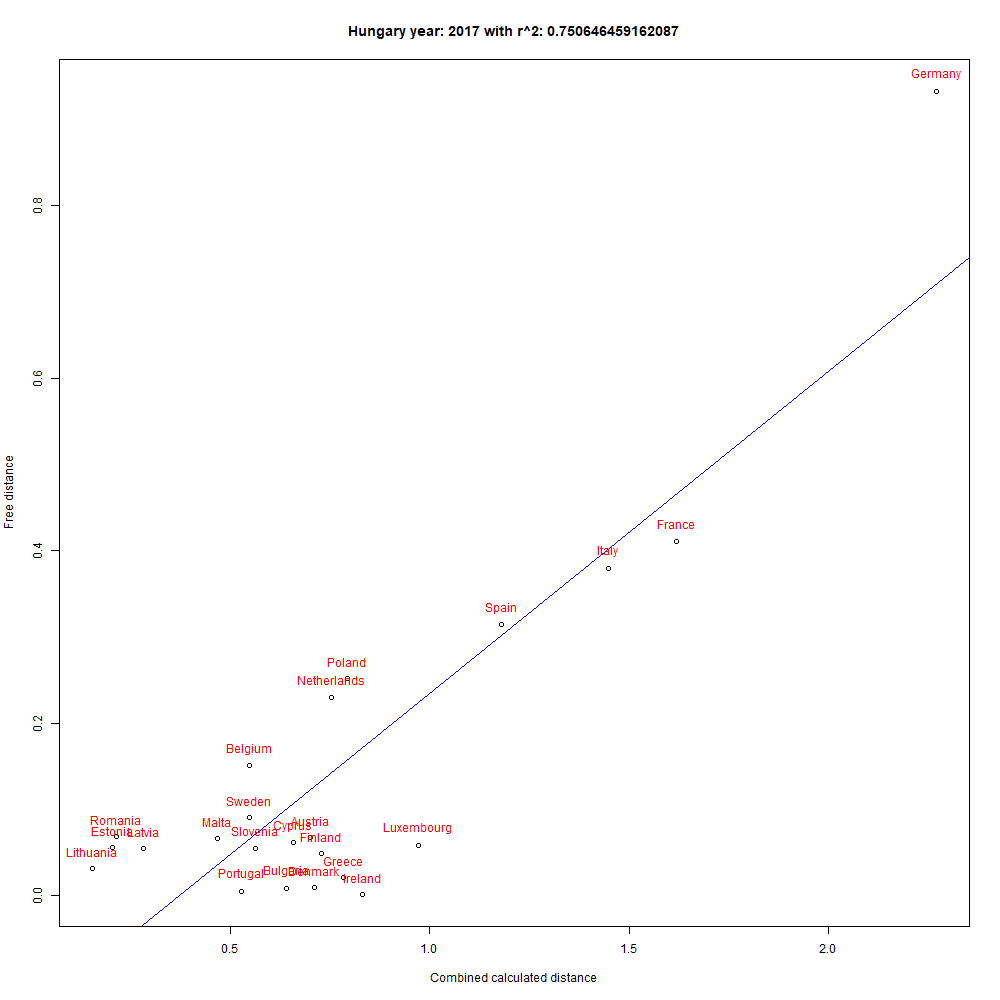
\includegraphics[width = \textwidth]{images/Hungary 2017.png}
		\caption{Hungary 2017}
		\label{fig:/Hungary_2017}
	\end{figure}
	\newpage
	Το οποίο μπορούμε να το αντιπαραθέσουμε με τις 3 άλλες χώρες που είδαμε και πριν.
	
	\begin{figure}[H]
		\centering
		\begin{subfigure}[b]{0.3\textwidth}
			\centering
			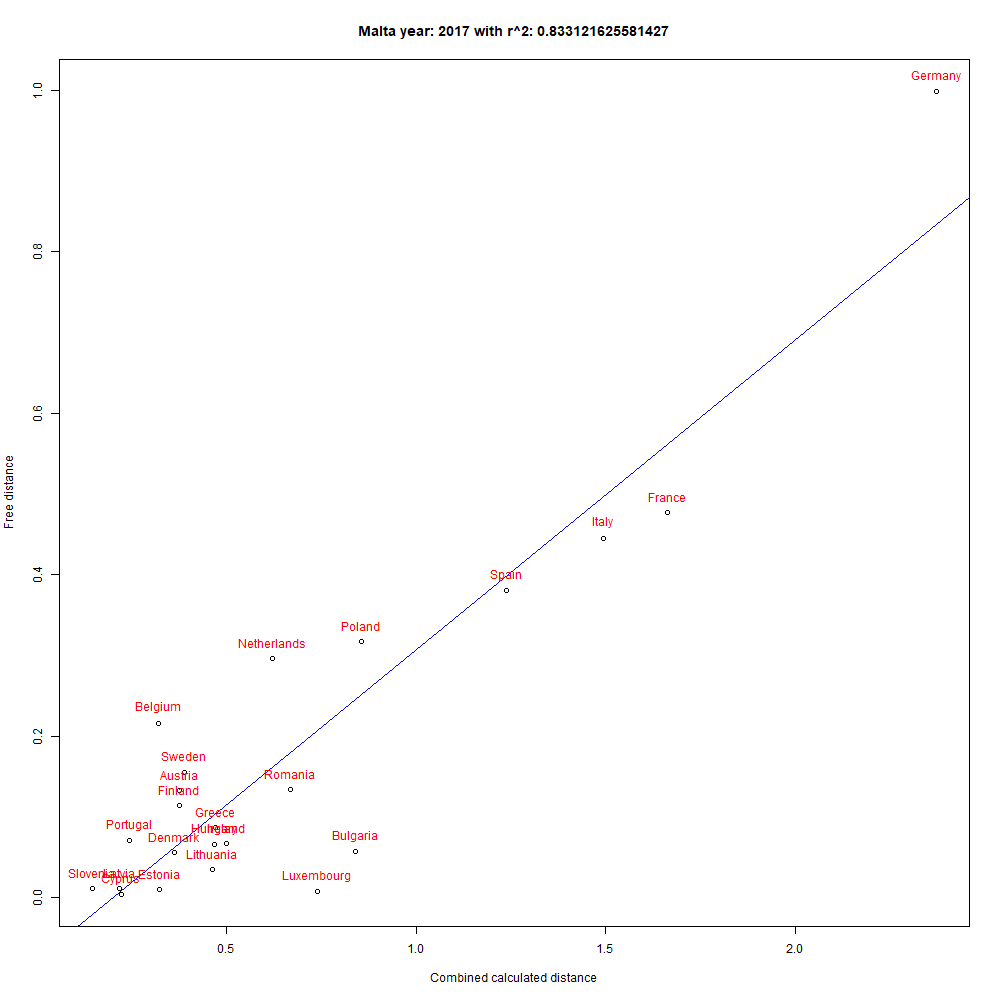
\includegraphics[width=\textwidth]{images/Malta 2017.png}
			\caption{Malta 2017}
			\label{fig:Malta_2017}
		\end{subfigure}
		\hfill
		\begin{subfigure}[b]{0.3\textwidth}
			\centering
			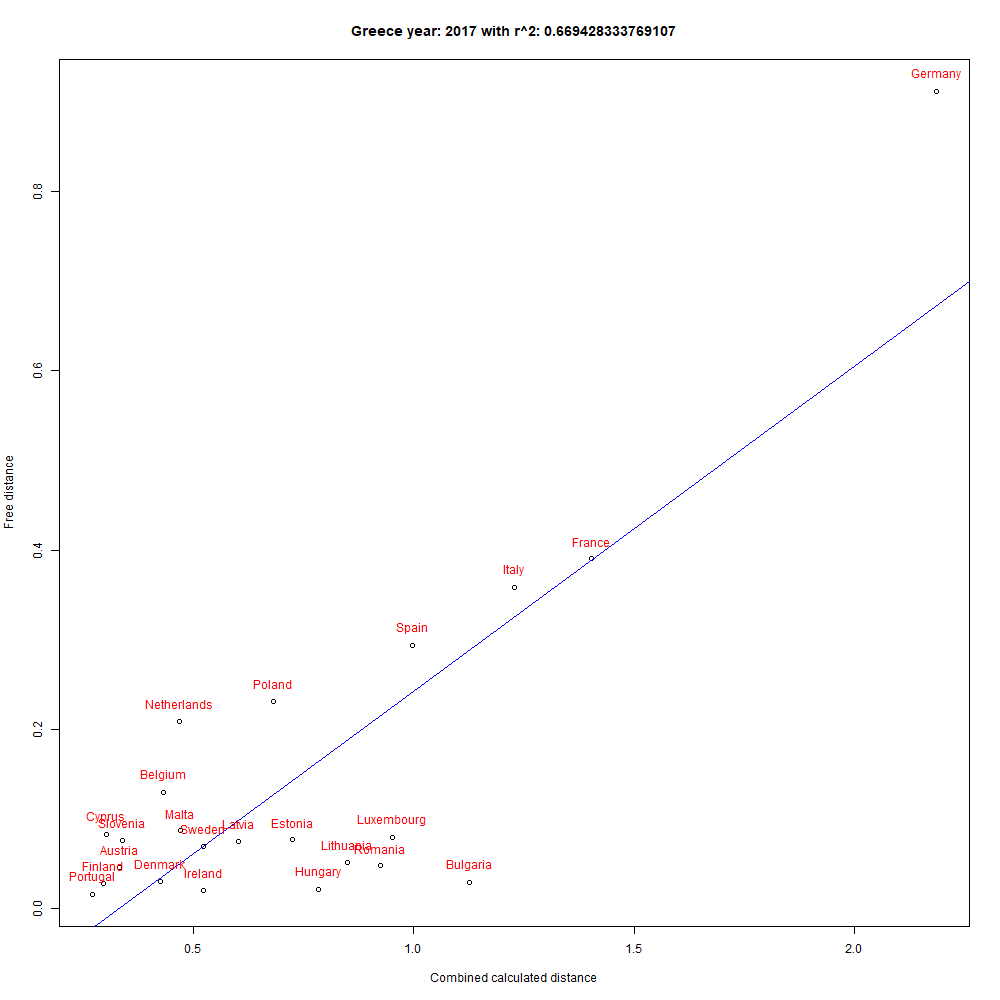
\includegraphics[width=\textwidth]{images/Greece 2017.png}
			\caption{Greece 2017}
			\label{fig:Greece_2017}
		\end{subfigure}
		\hfill
		\begin{subfigure}[b]{0.3\textwidth}
			\centering
			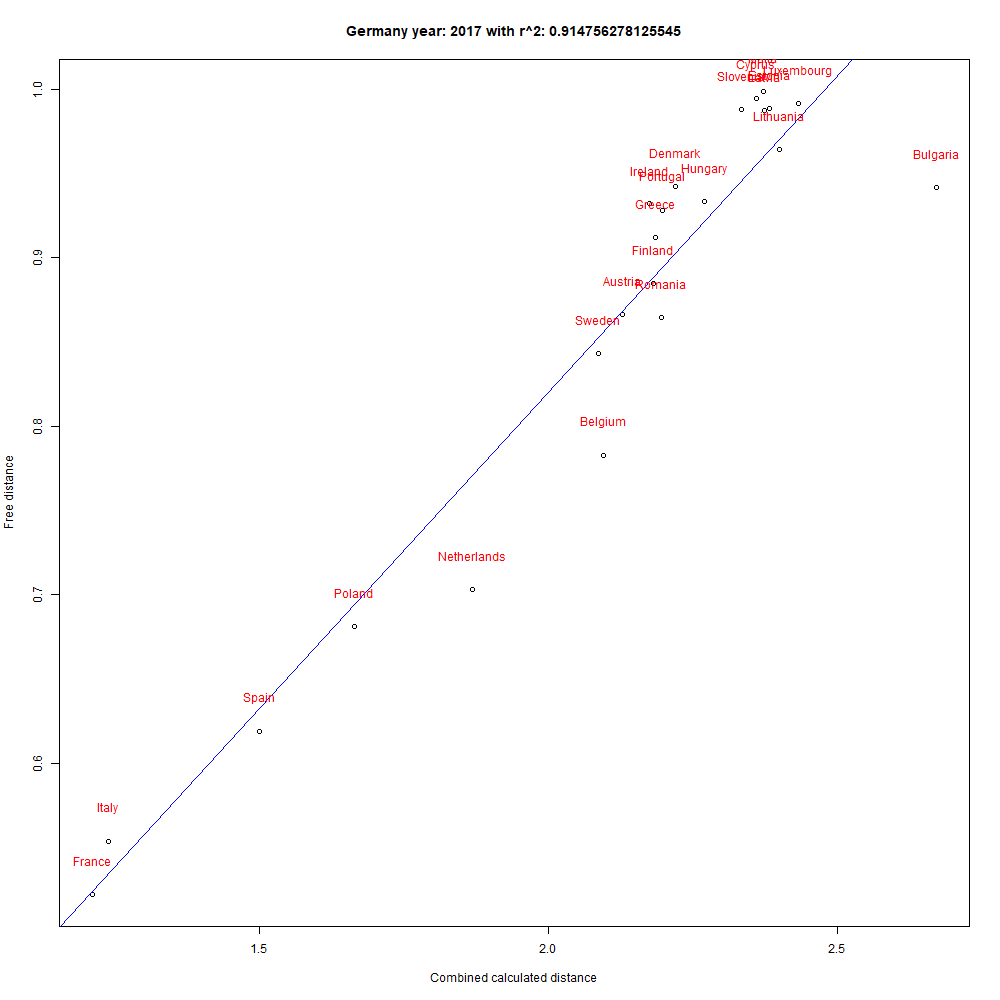
\includegraphics[width=\textwidth]{images/Germany 2017.png}
			\caption{Germany 2017}
			\label{fig:Germany_2017}
		\end{subfigure}
		%\caption{Αποστάσεις χωρών σε heatmap}
		\label{fig:3_examples}
	\end{figure}
	
	Παράλληλα μπορούμε να δούμε μέσα στις χρονιές επαναλαμβάνοντας το ίδιο πείραμα για όλες τις χώρες, τι θα προκύψει. 
	
	\begin{table}[ht]
		\centering
		\begin{tabular}{r|rrrrr}
			\hline
			year & slope & mean r\_squared & min\_r\_squared & max\_r\_squared \\
			\hline
			2008 & 0.34 & 0.65 & 0.00 & 0.79 \\
			2009 & 0.32 & 0.60 & 0.02 & 0.78 \\
			2010 & 0.33 & 0.58 & 0.04 & 0.79 \\
			2011 & 0.33 & 0.62 & 0.04 & 0.78 \\
			2012 & 0.34 & 0.64 & 0.07 & 0.82 \\
			2013 & 0.37 & 0.72 & 0.51 & 0.92 \\
			2014 & 0.36 & 0.71 & 0.46 & 0.93 \\
			2015 & 0.37 & 0.75 & 0.48 & 0.94 \\
			2016 & 0.35 & 0.70 & 0.50 & 0.91 \\
			2017 & 0.36 & 0.73 & 0.47 & 0.91 \\
			2018 & 0.37 & 0.74 & 0.43 & 0.92 \\
			\hline
		\end{tabular}
	\end{table}
	Συμπεράσματα:
	\begin{itemize}
		\item Η κλίση αυτής της ευθείας δείχνει να παραμένει πολύ σταθερή
		\item Μέχρι το 2012 (δηλαδή και το τέλος της φάσης ΙΙ) βλέπουμε πως υπάρχουν χώρες για τις οποίες δεν ισχύει το συμπέρασμα το οποίο είχαμε βγάλει, περί δικαιότητας του συστήματος.
		\item Μετά τη φάση ΙΙΙ ακόμα υπάρχουν χώρες για τις οποίες η μέθοδος αυτή δε δίνει σημαντικά καλές τιμές. 
	\end{itemize}
	\newpage
	
	Ένα ερώτημα που νομίζω πως είναι λογικό να προκύψει ξαφνικά είναι το "ποιο κρητήριο κάνει μία χώρα να είναι κατάλληλη για αυτή τη δουλειά; Πότε μπορούμε να διαλέξουμε μία χώρα για να είναι χρήσιμες οι αποστάσεις της;". Οπότε τα βάζουμε όλα μαζί στο ίδιο γράφημα και έχουμε:
	
	\begin{figure}[H]
		\centering
		
\includegraphics[width = \textwidth]{images/2017 r^2 vs GDP.png}
		\caption{2017 r\^2 vs GDP}
		\label{fig:/2017 r^2 vs_GDP}
	\end{figure}
	
	Δοκιμάζοντας και άλλα χαρακτηριστικά δεν κατέληξα σε κάτι πιο ενδιαφέρον από το παραπάνω διάγραμμα. Η Γερμανία δείχνει να είναι πολύ καλή για να κάνουμε αυτή τη δουλειά, μάλλον γιατί στον "χώρο των αποστάσεων" είναι τόσο μακριά από όλους τους άλλους που οι υπόλοιποι καταλήγουν να είναι συγκριτικά κοντά. Αυτό το λέω σαν διαισθητική παρατήρηση, δεν ξέρω αν στηρίζεται μαθηματικά. 
	
	Το επόμενο βήμα είναι να δούμε το προηογούμενο με τα βέλτιστα βάρη. 
	
	\section{ΓιΑ την 28η Φεβρουαρίου}
	
	Την τελευταία φορά προτείναμε να κάνουμε/δούμε/διαβάσουμε, χωρίς κάποια σειρά:
	\begin{enumerate}
		\item Να διαβάσω τον αλγόριθμο του benchmark, πώς προκύπτει ακριβώς.
		\item Να εξετάσουμε αν τα αποτελέσματα σχετικά με το "ποιες χώρες εξηγούν καλύτερα τα δεδομένα είναι consistant μέσα στον χρόνο.
		\item Υπάρχει κάποιο clustering μεταξύ των χωρών που εξηγούν καλά ή κακά τις άλλες χώρες; Έχουν κάποια κοινά χαρακτηριστικά όλες αυτές;
		\item Γιατί είναι η Ολλανδία τόσο διαφορετική;
		\item Να επαναληφθούν οι δοκιμές της προηγούμενη φοράς, αλλά για τις φάσεις 1,2 ( πιθανώς θα προκύψει πρόβλημα με τα δεδομένα για αυτές τις περιόδους, αλλά θα το δούμε)
		\item Κάνε δοκιμές και με μία fictional χώρα η οποία να έχει ως τιμές της μόνο τα medians όλων των χωρών. 
		\item Να γίνει καλύτερα η σύγκριση μεταξύ κάθε δύο παλινδρομήσεων, αξιολογώντας και το $r^2$, αλλά και άλλες παραμέτρους, όπως το p-value και MSE/MAE.
		\item Τι συμβαίνει στα πρώτα χρόνια με την Πολωνία και την Γαλλία;
		\item Να χρησιμοποιηθεί ggplot για τα δραγράμματα και να έχουν πάντα grid.
		\item Για διάβασμα : A multi-xriteria decision analysis model for carbon emission quota allocation in China's east coastal areas: Efficiency and Equity.
		
	\end{enumerate}
	
	\subsection{Αλλαγή 1}
	Το πρώτο βήμα που έγινε είναι το να ξαναγίνουν πολλά από τα πειράματα, μόνο που αυτή τη φορά, για να θεωρηθεί μία γραμμική παλινδρόμηση καλύτερη από μία άλλη, θα πρέπει να είναι αληθή τα παρακάτω κριτήρια:
	\begin{itemize}
		\item Εχει μεγαλύτερο $r^2$.
		\item Έχει p-value μικρότερο του 0.05.
		\item To Mean Square Error δεν είναι πολύ μεγαλύτερο από την προηγούμενη μέγιστη τιμή (1.5 φορά).
	\end{itemize}
	
	\subsection{Μεσαία χώρα ανά τα έτη}
	Εδώ βλέπουμε την πιο μεσαία χώρα κάθε χρονιάς και το πόσο καλά αποδίδει στο να εξηγεί τις άλλες χώρες. Οι τιμές στο p-value βγήκαν όντως 0, η μεγαλύτερη είχε την τιμή 0.00002581...
	\begin{table}[H]
		\centering
		\begin{tabular}{r|rrrrl}
			\hline
			Year & R\verb|^|2 & p-value & MSE & Country \\
			\hline
			2008 & 0.77 & 0.00 & 0.01 & Denmark \\ 
			2009 & 0.69 & 0.00 & 0.01 & Denmark \\
			2010 & 0.57 & 0.00 & 0.01 & Greece \\
			2011 & 0.65 & 0.00 & 0.02 & Denmark \\
			2012 & 0.75 & 0.00 & 0.01 & Ireland \\
			2013 & 0.71 & 0.00 & 0.01 & Portugal \\
			2014 & 0.58 & 0.00 & 0.02 & Hungary \\ 
			2015 & 0.77 & 0.00 & 0.01 & Portugal \\
			2016 & 0.70 & 0.00 & 0.01 & Portugal \\
			2017 & 0.75 & 0.00 & 0.01 & Hungary \\
			2018 & 0.74 & 0.00 & 0.01 & Hungary \\ 
			\hline
		\end{tabular}
	\end{table}
	\subsection{Όλες οι χώρες για όλα τα έτη}
	
	
	\begin{table}[H]
		\centering
		\tabcolsep=0.11cm
		\begin{tabular}{rrrrrrrrrrrrrr}
			\hline
			& 2008 & 2009 & 2010 & 2011 & 2012 & 2013 & 2014 & 2015 & 2016 & 2017 & 2018 & max p-value & max MSE \\ 
			\hline
			Austria & 0.70 & 0.62 & 0.66 & 0.68 & 0.71 & 0.74 & 0.73 & 0.82 & 0.72 & 0.68 & 0.74 & 0.00 & 0.02 \\ 
			Belgium & 0.62 & 0.62 & 0.62 & 0.64 & 0.65 & 0.67 & 0.67 & 0.65 & 0.57 & 0.60 & 0.59 & 0.00 & 0.01 \\
			Bulgaria & 0.75 & 0.67 & 0.73 & 0.67 & 0.78 & 0.84 & 0.85 & 0.86 & 0.69 & 0.81 & 0.85 & 0.00 & 0.01 \\
			Cyprus & 0.79 & 0.71 & 0.69 & 0.71 & 0.78 & 0.67 & 0.58 & 0.73 & 0.72 & 0.75 & 0.78 & 0.00 & 0.02 \\ 
			Denmark & 0.77 & 0.69 & 0.61 & 0.65 & 0.74 & 0.71 & 0.72 & 0.73 & 0.72 & 0.68 & 0.69 & 0.00 & 0.02 \\
			Estonia & 0.79 & 0.74 & 0.67 & 0.69 & 0.66 & 0.64 & 0.68 & 0.78 & 0.68 & 0.82 & 0.81 & 0.00 & 0.02 \\ 
			Finland & 0.71 & 0.64 & 0.66 & 0.73 & 0.68 & 0.73 & 0.77 & 0.80 & 0.72 & 0.69 & 0.76 & 0.00 & 0.01 \\
			\rowcolor{lightgray} France & 0.08 & 0.08 & 0.20 & 0.19 & 0.25 & 0.78 & 0.79 & 0.78 & 0.78 & 0.73 & 0.76 & 0.19 & 0.01 \\
			Germany & 0.76 & 0.75 & 0.79 & 0.76 & 0.80 & 0.92 & 0.93 & 0.94 & 0.91 & 0.91 & 0.92 & 0.00 & 0.01 \\
			Greece & 0.62 & 0.57 & 0.57 & 0.60 & 0.57 & 0.51 & 0.46 & 0.69 & 0.65 & 0.67 & 0.71 & 0.00 & 0.02 \\ 
			Hungary & 0.74 & 0.52 & 0.58 & 0.69 & 0.69 & 0.67 & 0.58 & 0.78 & 0.73 & 0.75 & 0.74 & 0.00 & 0.02 \\
			Ireland & 0.70 & 0.76 & 0.47 & 0.70 & 0.75 & 0.73 & 0.69 & 0.77 & 0.73 & 0.63 & 0.64 & 0.00 & 0.02 \\
			Italy & 0.63 & 0.61 & 0.65 & 0.64 & 0.60 & 0.86 & 0.82 & 0.75 & 0.74 & 0.72 & 0.78 & 0.00 & 0.01 \\ 
			Latvia & 0.76 & 0.70 & 0.62 & 0.66 & 0.68 & 0.77 & 0.74 & 0.75 & 0.78 & 0.84 & 0.81 & 0.00 & 0.02 \\
			Lithuania & 0.77 & 0.78 & 0.63 & 0.70 & 0.74 & 0.79 & 0.76 & 0.74 & 0.74 & 0.79 & 0.81 & 0.00 & 0.02 \\
			Luxembourg & 0.79 & 0.67 & 0.59 & 0.77 & 0.73 & 0.68 & 0.65 & 0.75 & 0.60 & 0.74 & 0.70 & 0.00 & 0.02 \\ 
			Malta & 0.76 & 0.65 & 0.62 & 0.68 & 0.78 & 0.75 & 0.72 & 0.82 & 0.71 & 0.83 & 0.82 & 0.00 & 0.02 \\
			Netherlands & 0.51 & 0.53 & 0.53 & 0.44 & 0.54 & 0.60 & 0.60 & 0.51 & 0.50 & 0.47 & 0.43 & 0.00 & 0.01 \\
			\rowcolor{lightgray} Poland & 0.00 & 0.02 & 0.04 & 0.04 & 0.07 & 0.60 & 0.60 & 0.48 & 0.54 & 0.69 & 0.69 & 0.92 & 0.02 \\
			Portugal & 0.71 & 0.66 & 0.66 & 0.60 & 0.59 & 0.71 & 0.73 & 0.77 & 0.70 & 0.75 & 0.77 & 0.00 & 0.02 \\ 
			Romania & 0.53 & 0.46 & 0.42 & 0.58 & 0.45 & 0.60 & 0.75 & 0.80 & 0.64 & 0.66 & 0.67 & 0.00 & 0.01 \\
			Slovenia & 0.78 & 0.59 & 0.59 & 0.67 & 0.70 & 0.76 & 0.73 & 0.77 & 0.78 & 0.78 & 0.81 & 0.00 & 0.02 \\ 
			Spain & 0.63 & 0.61 & 0.63 & 0.57 & 0.60 & 0.84 & 0.74 & 0.76 & 0.72 & 0.77 & 0.81 & 0.00 & 0.01 \\
			Sweden & 0.70 & 0.56 & 0.61 & 0.59 & 0.67 & 0.74 & 0.75 & 0.81 & 0.75 & 0.77 & 0.77 & 0.00 & 0.02 \\ 
			United Kingdom & 0.75 & 0.71 & 0.77 & 0.78 & 0.82 & 0.63 & 0.69 & 0.66 & 0.66 & 0.72 & 0.71 & 0.00 & 0.01 \\
			\hline
		\end{tabular}
	\end{table}
	Το οποίο γραφικά φαίνεται και ως εξής:
	\begin{figure}[H]
		\centering
		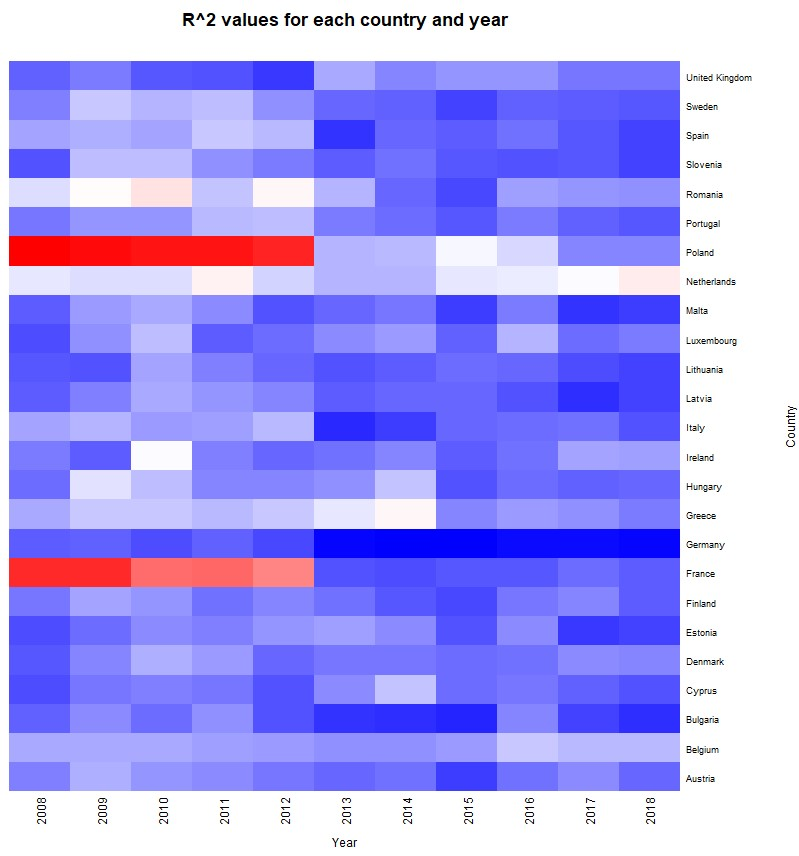
\includegraphics[width = \textwidth]{images/plot.jpg}
		\caption{$r^2$}
		\label{fig:/2017 r^2 vs GDP}
	\end{figure}
	
	Το πιο λογικό λοιπόν βήμα είναι το να ελέγξουμε το γιατί αυτές οι δύο χώρες αλλάζουν τόσο πολύ το 2013. Οπότε ας δούμε τα δεδομένα που χρησιμοποιούμε για αυτές:
	\begin{table}[H]
		\centering
		\begin{tabular}{rllll}
			\hline
			& 2012 & 2013 & 2012 & 2013 \\
			\hline
			GEO & Poland & Poland & France & France \\
			Total\_energy\_supply & 0.3083121 & 0.3038433 & 0.8215192 & 0.8080548 \\ 
			GDPpc & 0.1163326 & 0.1141371 & 0.3630366 & 0.3550416 \\
			Population & 0.4732704 & 0.4716958 & 0.8164021 & 0.8183792 \\
			Inflation & 0.57990986 & 0.07563843 & 0.28530815 & 0.19301719 \\ 
			Verified\_emissions & 0.4212666 & 0.4212431 & 0.2421093 & 0.2422275 \\
			Agriculture & 0.3402106 & 0.3644831 & 1.0000000 & 0.8928814 \\
			Industry & 0.1558893 & 0.1482026 & 0.4982965 & 0.5053396 \\
			Manufacturing & 0.1166064 & 0.1091561 & 0.3911272 & 0.3913494 \\ 
			\hline
		\end{tabular}
	\end{table}
	Όπως είναι εμφανές, στα δεδομένα των χωρών δεν υπάρχει κάτι προφανές το οποίο να δικαιολογεί αυτήν την τόσο απότομη αλλαγή. Τα δεδομένα τα βλέπουμε κανονικοποιημένα.
	
	Επίσης, για το ποιες χώρες τα πηγαίνουν καλύτερα, μπορούμε ν αφτιάξουμε αυτήν την κατάταξη, η οποία είναι αρκετά αντιπροσωπευτική.
	\begin{table}[H]
		\centering
		\begin{tabular}{rlr}
			\hline
			& Country & Average R\verb|^|2 \\
			\hline
			1 & Germany & 0.85 \\
			2 & Bulgaria & 0.77 \\
			3 & Lithuania & 0.75 \\
			4 & Malta & 0.74 \\
			5 & Latvia & 0.74 \\ 
			6 & Estonia & 0.72 \\
			7 & Slovenia & 0.72 \\
			8 & Cyprus & 0.72 \\
			9 & United Kingdom & 0.72 \\
			10 & Finland & 0.72 \\
			11 & Italy & 0.71 \\
			12 & Austria & 0.71 \\
			13 & Sweden & 0.70 \\ 
			14 & Denmark & 0.70 \\
			15 & Spain & 0.70 \\
			16 & Luxembourg & 0.70 \\
			17 & Portugal & 0.70 \\
			18 & Ireland & 0.69 \\
			19 & Hungary & 0.68 \\
			20 & Belgium & 0.63 \\
			21 & Greece & 0.60 \\
			22 & Romania & 0.60 \\
			23 & Netherlands & 0.52 \\
			24 & France & 0.49 \\ 
			25 & Poland & 0.34 \\
			\hline
		\end{tabular}
	\end{table}

	\newpage
	\section{Για τη 14η Μαρτίου}
	
	Είπαμε να διορθωθούν τα παρακάτω:
	\begin{itemize}
		\item Οι πίνακες με δεδομένα να έχουν 2 δεκαδικά ψηφία ή όσα είναι αναγκαία, όχι παραπάνω.
		\item Να προστίθενται γραμμές στις αναφορές ανά 5 στοιχεία, ώστε να είναι ευδιάκριτα τα νούμερα.
		\item Να φτιαχτεί ένα πινακάκι με descriptive statistics για τα δεδομένα τα οποία έχουμε, να περιλαμβάνει min, max, quantiles, median και boxplot.
		\item Να γίνει η παραπάνω παρουσίαση για τα αρχικά δεδομένα, αλλά και για τα κανονικοποιημένα δεδομένα.
		\item Πιθανώς να δούμε την διαφορά που θα είχε η χρήση κάποιου διαφορετικού τρόπου κανονικοποίησης. (Μέχρι τώρα η κανονικοποίηση γίνεται διαιρώντας με την μέγιστη τιμή. Ένας άλλος τρόπος θα ήταν ο $\frac{X- X_{min}}{X_{max}- X_{min}}$)
	\end{itemize}
	
	
	\subsection{Πίνακας $r^2$ με βέλτιστα επιλεγμένα βάρη}
	Εδώ φαίνεται ο πίνακας της προηγούμενης εβδομάδας, με την διαφορά ότι κάθε χώρα μπορούσε να επιλέξει το "mix" δεδομένων που θα χρησιμοποιήσει ώστε να είναι βέλτιστο το $r^2$. Εδώ βλέπουμε πως η Γαλλία έχει  πολύ πιο μικρό πρόβλημα. 
	
	Ο αλγόριθμος ο οποίος χρησιμοποιήθηκε για να βγει αυτός ο πίνακας είναι πολύ κακός. Θεωρεί πως υπάρχει κάποια γραμμική συσχέτιση της ικανότητας μίας χώρας να περιγράψει τις άλλες και του βάρους κάθε διαφορετικού δεδομένου (για παράδειγμα, τα verfied emissions έχουν μία γνησίως αύξουσα σχέση με την ικανότητα της χώρας να περιγράψει τις άλλες.) Αυτό δεν ισχύει και ίσως είναι ενδιαφέρον το να δούμε πώς μοιάζει η συνάρτηση αυτή. 
	
	Πάντως ο αλγόριθμος αυτός κάνει τα παρακάτω:
	\begin{enumerate}
		\item Διαλέγει ένα από τα βάρη των διαφορετικών δεδομένων.
		\item Δοκιμαστικά "ανεβάζει" και "κατεβάζει" το αντίστοιχο βάρος και βλέπει ποιο οδηγεί σε καλύτερη παλινδρόμηση.
		\item Επαναλαμβάνει το προηγούμενο βήμα μέχρι να χτηπίσει κάποιο όριο ή να είναι χειρότερες και οι δύο επιλογές.
		\item Προχωρά στο επόμενο βάρος το οποίο μπορεί να βελτιστοποιήσει.
		\item Οι παράμετροι ήταν:
		\begin{itemize}
			\item Ελάχιστο βάρος: 0
			\item Μέγιστο βάρος: 1000
			\item Βήμα: 10
			\item Τιμή εκκίνησης: 50
			\item Υπάρχουν 8 βάρη, τυχαία διαλέγει το βάρος το οποίο θα προσπαθήσει να βελτιστοποιήσει 100 φορές 
		\end{itemize}
	\end{enumerate}
	 
	\begin{table}[H]
		\centering
		\tabcolsep=0.11cm
		\begin{tabular}{r|rrrrr|rrrrrr|rr}
			\hline
			& 2008 & 2009 & 2010 & 2011 & 2012 & 2013 & 2014 & 2015 & 2016 & 2017 & 2018 & max p-value & max MSE \\ 
			\hline
			Austria & 0.99 & 0.98 & 0.98 & 0.98 & 0.99 & 0.98 & 0.98 & 0.98 & 0.98 & 0.97 & 0.97 & 0.00 & 0.00 \\ 
			Belgium & 0.98 & 0.98 & 0.98 & 0.99 & 0.98 & 0.91 & 0.90 & 0.91 & 0.89 & 0.88 & 0.89 & 0.00 & 0.00 \\ 
			Bulgaria & 0.98 & 0.98 & 0.98 & 0.98 & 0.99 & 0.97 & 0.97 & 0.97 & 0.97 & 0.97 & 0.97 & 0.00 & 0.00 \\ 
			Cyprus & 0.99 & 0.98 & 0.98 & 0.98 & 0.99 & 0.97 & 0.96 & 0.97 & 0.97 & 0.97 & 0.97 & 0.00 & 0.00 \\ 
			Denmark & 0.99 & 0.98 & 0.97 & 0.98 & 0.99 & 0.97 & 0.97 & 0.97 & 0.97 & 0.97 & 0.96 & 0.00 & 0.00 \\ 
			Estonia & 0.99 & 0.98 & 0.98 & 0.98 & 0.98 & 0.96 & 0.97 & 0.97 & 0.97 & 0.97 & 0.97 & 0.00 & 0.00 \\ 
			Finland & 0.99 & 0.98 & 0.98 & 0.98 & 0.98 & 0.97 & 0.98 & 0.97 & 0.98 & 0.97 & 0.97 & 0.00 & 0.00 \\ 
			\rowcolor{cyan} France & 0.08 & 0.08 & 0.97 & 0.96 & 0.98 & 0.98 & 0.98 & 0.96 & 0.98 & 0.98 & 0.98 & 0.19 & 0.01 \\ 
			Germany & 1.00 & 0.99 & 0.99 & 0.99 & 0.99 & 0.98 & 0.98 & 0.98 & 0.98 & 0.97 & 0.98 & 0.00 & 0.00 \\ 
			Greece & 0.98 & 0.98 & 0.98 & 0.98 & 0.98 & 0.96 & 0.96 & 0.97 & 0.98 & 0.97 & 0.97 & 0.00 & 0.00 \\ 
			Hungary & 0.99 & 0.97 & 0.97 & 0.98 & 0.98 & 0.97 & 0.96 & 0.97 & 0.97 & 0.97 & 0.97 & 0.00 & 0.00 \\ 
			Ireland & 0.99 & 0.98 & 0.97 & 0.99 & 0.99 & 0.97 & 0.97 & 0.97 & 0.97 & 0.96 & 0.96 & 0.00 & 0.00 \\ 
			Italy & 0.96 & 0.93 & 0.97 & 0.98 & 0.99 & 0.96 & 0.96 & 0.97 & 0.97 & 0.97 & 0.96 & 0.00 & 0.00 \\ 
			Latvia & 0.98 & 0.98 & 0.97 & 0.98 & 0.98 & 0.97 & 0.97 & 0.97 & 0.98 & 0.98 & 0.97 & 0.00 & 0.00 \\ 
			Lithuania & 0.99 & 0.98 & 0.97 & 0.98 & 0.99 & 0.98 & 0.98 & 0.98 & 0.98 & 0.98 & 0.97 & 0.00 & 0.00 \\ 
			Luxembourg & 0.98 & 0.97 & 0.97 & 0.98 & 0.98 & 0.96 & 0.96 & 0.97 & 0.97 & 0.97 & 0.97 & 0.00 & 0.00 \\ 
			Malta & 0.99 & 0.98 & 0.97 & 0.98 & 0.99 & 0.97 & 0.97 & 0.97 & 0.97 & 0.98 & 0.97 & 0.00 & 0.00 \\ 
			Netherlands & 0.97 & 0.97 & 0.97 & 0.97 & 0.98 & 0.81 & 0.81 & 0.80 & 0.79 & 0.73 & 0.69 & 0.00 & 0.00 \\ 
			\rowcolor{cyan} Poland & 0.00 & 0.02 & 0.04 & 0.04 & 0.07 & 0.94 & 0.94 & 0.94 & 0.95 & 0.95 & 0.94 & 0.92 & 0.02 \\ 
			Portugal & 0.99 & 0.98 & 0.98 & 0.98 & 0.98 & 0.97 & 0.98 & 0.97 & 0.98 & 0.97 & 0.97 & 0.00 & 0.00 \\ 
			Romania & 0.95 & 0.95 & 0.93 & 0.96 & 0.96 & 0.98 & 0.98 & 0.98 & 0.97 & 0.97 & 0.97 & 0.00 & 0.00 \\ 
			Slovenia & 0.99 & 0.97 & 0.97 & 0.98 & 0.98 & 0.97 & 0.97 & 0.97 & 0.97 & 0.97 & 0.97 & 0.00 & 0.00 \\ 
			Spain & 0.98 & 0.97 & 0.98 & 0.97 & 0.98 & 0.95 & 0.94 & 0.95 & 0.95 & 0.95 & 0.95 & 0.00 & 0.00 \\ 
			Sweden & 0.99 & 0.98 & 0.97 & 0.98 & 0.99 & 0.97 & 0.98 & 0.98 & 0.97 & 0.97 & 0.97 & 0.00 & 0.00 \\ 
			United Kingdom & 0.99 & 0.99 & 0.99 & 0.99 & 0.99 & 0.92 & 0.94 & 0.97 & 0.98 & 0.98 & 0.98 & 0.00 & 0.00 \\ 
			\hline
		\end{tabular}
	\end{table}
	Σε αυτόν τον πίνακα τα μέσα βάρη ήταν:
	\begin{itemize}
		\item Population: 59.63
		\item GDP per capita: 19.85
		\item Inflation: 15.12
		\item Agriculture: 69.09
		\item Industry: 407.60
		\item Manufacturing: 12.69
		\item Total energy supply: 170.25
		\item Verified emissions: 849.81\\
	\end{itemize}
\newpage
\subsection{Οπτικοποίηση δεδομένων}
\subsubsection{Πληθυσμός}
	\begin{itemize}
	\item Source: https://data.worldbank.org/indicator/SP.POP.TOTL
	\item Year: 2011 - 2021
	\item Unit: Persons
\end{itemize}   
Για τον πληθυσμό δεν έχω τίποτα εντυπωσιακό να πω. Ίσως είναι κάπως εύκολο να δούμε όλα τα δεδομένα ταυτόχρονα και να παρατηρήσουμε τι αλλαγή επιφέρει η κανονικοποίηση στα δεδομένα. Όπως φαίνεται στα figure 7 και 8. Τα σχήματα είναι ολόιδια. Η διαφορά είναι πως το ένα έχει διαιρεθεί με το 1000000 ενώ το άλλο έχει διαιρεθεί με το μέγιστο κάθε χρονιάς, οπότε είναι ελαφρώς διαφορετικές οι σχέσεις μεταξύ των αριθμών κάθε χώρας. 

\begin{table}[H]
	\centering
	\begin{tabular}{|r|rrrrr|r|}
		\hline
		Population & min & 25-quantile & median & 75-quantile & max & Std \\ 
		\hline
		Austria & 8.32 & 8.38 & 8.48 & 8.69 & 8.84 & 0.19 \\ 
		Belgium & 10.71 & 10.97 & 11.16 & 11.30 & 11.43 & 0.24 \\ 
		Bulgaria & 7.03 & 7.15 & 7.27 & 7.37 & 7.49 & 0.15 \\ 
		Cyprus & 1.08 & 1.12 & 1.14 & 1.17 & 1.19 & 0.03 \\ 
		Denmark & 5.49 & 5.56 & 5.61 & 5.71 & 5.79 & 0.10 \\
		\hline 
		Estonia & 1.31 & 1.32 & 1.32 & 1.33 & 1.34 & 0.01 \\ 
		Finland & 5.31 & 5.38 & 5.44 & 5.49 & 5.52 & 0.07 \\ 
		France & 64.37 & 65.19 & 66.00 & 66.64 & 67.10 & 0.93 \\ 
		Germany & 80.27 & 80.81 & 81.78 & 82.23 & 82.91 & 0.91 \\ 
		Greece & 10.73 & 10.80 & 10.97 & 11.09 & 11.12 & 0.15 \\ 
		\hline
		Hungary & 9.78 & 9.83 & 9.89 & 9.99 & 10.04 & 0.09 \\ 
		Ireland & 4.49 & 4.57 & 4.62 & 4.73 & 4.87 & 0.12 \\ 
		Italy & 58.83 & 59.33 & 60.23 & 60.58 & 60.79 & 0.73 \\ 
		Latvia & 1.93 & 1.97 & 2.01 & 2.08 & 2.18 & 0.08 \\ 
		Lithuania & 2.80 & 2.89 & 2.96 & 3.06 & 3.20 & 0.13 \\ 
		\hline
		Luxembourg & 0.49 & 0.51 & 0.54 & 0.58 & 0.61 & 0.04 \\ 
		Malta & 0.41 & 0.42 & 0.43 & 0.45 & 0.48 & 0.03 \\ 
		Netherlands & 16.45 & 16.65 & 16.80 & 16.99 & 17.23 & 0.25 \\ 
		Poland & 37.97 & 37.98 & 38.04 & 38.06 & 38.15 & 0.06 \\ 
		Portugal & 10.28 & 10.34 & 10.46 & 10.56 & 10.57 & 0.12 \\ 
		\hline
		Romania & 19.47 & 19.76 & 19.98 & 20.20 & 20.54 & 0.33 \\ 
		Slovenia & 2.02 & 2.05 & 2.06 & 2.06 & 2.07 & 0.01 \\ 
		Spain & 45.95 & 46.46 & 46.58 & 46.68 & 46.80 & 0.24 \\ 
		Sweden & 9.22 & 9.41 & 9.60 & 9.86 & 10.18 & 0.31 \\ 
		United Kingdom & 61.81 & 63.01 & 64.13 & 65.36 & 66.46 & 1.55 \\ 
		\hline
	\end{tabular}
	\caption{Population in millions 2008-2018}
	\label{population}
\end{table}


Παράλληλα, μπορούμε να παρατηρήσουμε τα δεδομένα κάπως καλύτερα, όπου φαίνεται πως η κανονικοποίηση δεν επηρεάζει καθόλου την σχέση μεταξύ των τιμών:


\begin{figure}[H]
	\centering
	\begin{subfigure}[a]{0.8\textwidth}
		\centering
	\includegraphics[width=1\linewidth]{"images/Boxplot Population Normalized vs Country"}
	\caption{}
	\label{fig:boxplot-population-normalized-vs-country}
	\end{subfigure}
	\begin{subfigure}[b]{0.8\textwidth}
		\includegraphics[width=1\linewidth]{"images/Boxplot Population in Millions vs Country"}
		\caption{}
		\label{fig:boxplot-population-in-millions-vs-country}
	\end{subfigure}
\end{figure}
\subsubsection{Πληθωρισμός}
	\begin{itemize}
	\item Source: https://data.worldbank.org/indicator/FP.CPI.TOTL.ZG
	\item Year: 1960-2021
	\item Unit: \%
	\end{itemize}
\begin{table}[H]
	\centering
	\begin{tabular}{|r|rrrrr|r|}
\hline
		Inflation & min & 25-quantile & median & 75-quantile & max & Std \\ 
  \hline
Austria & 0.87 & 1.71 & 1.85 & 2.01 & 2.30 & 0.45 \\ 
Belgium & 0.53 & 1.30 & 1.81 & 1.90 & 1.96 & 0.47 \\ 
Bulgaria & 0.07 & 1.23 & 3.32 & 4.52 & 8.10 & 2.45 \\ 
Cyprus & -1.33 & -0.66 & 1.00 & 1.65 & 4.73 & 1.74 \\ 
Denmark & 0.25 & 0.58 & 0.89 & 1.78 & 4.13 & 1.27 \\ 
\hline
Estonia & -0.39 & 2.00 & 3.59 & 4.05 & 6.80 & 2.02 \\ 
Finland & 0.09 & 1.22 & 1.77 & 2.59 & 3.04 & 1.02 \\ 
France & 0.07 & 0.55 & 0.95 & 1.10 & 2.37 & 0.58 \\ 
Germany & 0.65 & 1.20 & 1.50 & 1.87 & 1.97 & 0.46 \\ 
Greece & -2.05 & -0.44 & -0.18 & 0.62 & 4.34 & 1.85 \\ 
\hline
Hungary & 1.32 & 2.66 & 2.89 & 4.11 & 4.85 & 1.15 \\ 
Ireland & -4.62 & -0.28 & 0.71 & 1.22 & 7.70 & 3.10 \\ 
Italy & 0.44 & 0.92 & 1.13 & 1.58 & 2.40 & 0.54 \\ 
Latvia & -9.67 & 0.49 & 1.92 & 3.77 & 11.65 & 5.17 \\ 
Lithuania & -3.30 & 1.06 & 2.53 & 3.88 & 9.71 & 3.30 \\ 
\hline
Luxembourg & -1.11 & 1.94 & 2.28 & 3.36 & 6.61 & 1.99 \\ 
Malta & 1.12 & 2.06 & 2.22 & 2.75 & 4.22 & 0.82 \\ 
Netherlands & 0.19 & 0.35 & 0.94 & 1.36 & 2.44 & 0.79 \\ 
Poland & 0.30 & 0.75 & 1.65 & 2.82 & 3.89 & 1.34 \\ 
Portugal & -0.39 & 0.67 & 1.51 & 1.78 & 2.25 & 0.90 \\ 
\hline
Romania & 1.80 & 3.33 & 3.77 & 4.38 & 16.02 & 3.88 \\ 
Slovenia & -1.03 & 0.68 & 1.04 & 1.86 & 4.47 & 1.49 \\ 
Spain & -0.22 & 0.06 & 0.32 & 0.90 & 2.25 & 0.76 \\ 
Sweden & 0.93 & 1.04 & 1.74 & 2.25 & 3.24 & 0.75 \\ 
United Kingdom & 0.51 & 1.60 & 1.82 & 2.03 & 3.23 & 0.65 \\ 
\hline
	\end{tabular}
	\caption{Πληθωρισμός μεταξύ 2008-2018}
	\label{Inflation}
\end{table}
Εδώ βέβαια ίσως έχει σημασία να δούμε λίγο τι συμβαίνει στα δεδομένα με την κανονικοποίηση. Ούτε εδώ αλλάζουν σημαντικά οι σχέσεις μεταξύ τους.
\begin{figure}[H]
	\centering
	\begin{subfigure}[]{0.8\textwidth}
		\centering
		\includegraphics[width=1\linewidth]{"images/boxplot\_inflation\_raw.png"}
		\caption{}
		\label{fig:boxplot-Inflation-normalized-vs-country}
	\end{subfigure}
	\begin{subfigure}[]{0.8\textwidth}
		\includegraphics[width=1\linewidth]{"images/boxplot\_inflation\_normalized.png"}
		\caption{}
		\label{fig:boxplot-inflation-vs-country}
	\end{subfigure}
\end{figure}
\subsubsection{Total energy Supply}
	\begin{itemize}
	\item Source: https://ec.europa.eu/eurostat/databrowser/view/nrg\_bal\_s\_1/default/table?lang=en
	\item Year: 2011 - 2020
	\item Unit: Thousand tonnes of oil equivalent
\end{itemize}
\begin{table}[H]
	\centering
	\begin{tabular}{|r|rrrrr|r|}
  \hline
& min & 25-quantile & median & 75-quantile & max & Std \\ 
\hline
Austria & 32011.29 & 33031.17 & 33177.75 & 33562.30 & 34166.28 & 660.54 \\ 
Belgium & 52238.38 & 53015.79 & 55039.87 & 55272.03 & 59313.06 & 2255.37 \\ 
Bulgaria & 16923.38 & 17726.43 & 18234.79 & 18722.35 & 19823.90 & 813.92 \\ 
Cyprus & 1955.96 & 2121.56 & 2262.44 & 2440.09 & 2616.93 & 221.87 \\ 
Denmark & 16374.16 & 16838.22 & 17383.65 & 18304.45 & 19558.31 & 1128.72 \\
  \hline 
Estonia & 4399.62 & 5378.58 & 5648.48 & 5846.32 & 5978.41 & 496.84 \\ 
Finland & 32022.99 & 33165.71 & 33582.86 & 34469.06 & 36251.74 & 1195.84 \\ 
France & 248383.41 & 250072.60 & 256292.91 & 259845.13 & 266394.54 & 6206.33 \\ 
Germany & 305036.83 & 310746.75 & 313107.91 & 318940.66 & 335474.27 & 9403.81 \\ 
Greece & 22748.62 & 23240.71 & 23407.97 & 27231.17 & 30404.91 & 2854.85 \\ 
  \hline
Hungary & 23652.51 & 24816.51 & 25609.63 & 26395.50 & 26900.70 & 1096.99 \\ 
Ireland & 12776.63 & 13293.33 & 13625.33 & 14225.86 & 15022.14 & 727.58 \\ 
Italy & 146769.88 & 152859.01 & 156093.49 & 168758.58 & 181736.20 & 10969.89 \\ 
Latvia & 4259.46 & 4307.46 & 4407.65 & 4465.42 & 4640.00 & 129.86 \\ 
Lithuania & 6946.51 & 7067.95 & 7290.53 & 7647.47 & 9553.50 & 819.46 \\ 
  \hline
Luxembourg & 3682.05 & 3785.50 & 3948.40 & 4127.44 & 4212.94 & 195.48 \\ 
Malta & 594.33 & 687.68 & 780.25 & 834.21 & 881.48 & 97.20 \\ 
Netherlands & 71379.09 & 73882.75 & 75619.51 & 77123.41 & 82743.78 & 3132.34 \\ 
Poland & 93773.11 & 96236.75 & 97971.41 & 101131.11 & 108970.23 & 4555.35 \\ 
Portugal & 21439.29 & 22060.46 & 22651.14 & 23433.93 & 24716.20 & 1092.37 \\
  \hline 
Romania & 31378.66 & 31668.07 & 33454.78 & 34845.41 & 39485.27 & 2432.37 \\ 
Slovenia & 6473.51 & 6722.90 & 6875.85 & 7127.16 & 7982.69 & 419.35 \\ 
Spain & 114522.76 & 119335.11 & 125486.61 & 126434.02 & 138166.04 & 6411.76 \\ 
Sweden & 44092.81 & 48432.69 & 49103.98 & 49874.22 & 50118.89 & 1857.82 \\ 
United Kingdom & 174024.39 & 177000.66 & 186386.17 & 191789.70 & 208268.88 & 11384.30 \\ 
\hline
	\end{tabular}
	\caption{Total energy supply μεταξύ 2008-2018}
	\label{Total energy Supply}
\end{table}

\subsubsection{GDP per capita}
	\begin{itemize}
	\item Source: https://data.worldbank.org/indicator/NY.GDP.PCAP.CD
	\item Year: 1960 - 2021
	\item Unit: US\$
\end{itemize}

\begin{table}[H]
	\centering
	\begin{tabular}{|r|rrrrr|r|}
  \hline
& min & 25-quantile & median & 75-quantile & max & Std \\ 
\hline
Austria & 44.20 & 47.17 & 48.56 & 51.46 & 51.92 & 2.75 \\ 
Belgium & 41.01 & 44.19 & 44.76 & 47.48 & 48.30 & 2.43 \\ 
Bulgaria & 6.85 & 7.17 & 7.57 & 7.88 & 9.45 & 0.74 \\ 
Cyprus & 23.41 & 26.89 & 28.91 & 31.57 & 35.40 & 3.57 \\ 
Denmark & 53.25 & 57.83 & 58.51 & 61.67 & 64.32 & 3.39 \\ 
\hline
Estonia & 14.66 & 17.40 & 18.20 & 19.66 & 23.06 & 2.45 \\ 
Finland & 42.80 & 46.46 & 47.71 & 50.16 & 53.77 & 3.25 \\ 
France & 36.65 & 39.73 & 41.59 & 42.84 & 45.52 & 2.75 \\ 
Germany & 41.10 & 41.89 & 44.65 & 46.50 & 48.02 & 2.61 \\ 
Greece & 17.92 & 19.17 & 21.79 & 26.10 & 32.13 & 4.84 \\ \hline
Hungary & 12.72 & 13.09 & 13.72 & 14.46 & 16.43 & 1.21 \\ 
Ireland & 48.66 & 51.83 & 55.60 & 62.44 & 79.11 & 9.57 \\ 
Italy & 30.24 & 33.51 & 35.56 & 36.63 & 40.94 & 3.17 \\ 
Latvia & 11.42 & 13.56 & 14.33 & 15.72 & 17.87 & 1.87 \\ 
Lithuania & 11.82 & 14.32 & 14.94 & 16.14 & 19.19 & 2.11 \\ \hline
Luxembourg & 105.46 & 109.81 & 112.58 & 119.51 & 123.68 & 6.14 \\ 
Malta & 21.08 & 22.37 & 24.77 & 26.19 & 31.57 & 3.23 \\ 
Netherlands & 45.19 & 49.37 & 52.20 & 52.97 & 57.88 & 3.66 \\ 
Poland & 11.53 & 12.60 & 13.70 & 13.94 & 15.47 & 1.08 \\ 
Portugal & 19.25 & 21.03 & 22.10 & 23.18 & 24.95 & 1.68 \\ \hline
Romania & 8.21 & 8.76 & 9.55 & 10.24 & 12.40 & 1.23 \\ 
Slovenia & 20.89 & 23.07 & 23.53 & 24.96 & 27.60 & 1.92 \\ 
Spain & 25.74 & 28.25 & 29.50 & 31.11 & 35.51 & 2.74 \\ 
Sweden & 46.95 & 52.42 & 54.59 & 59.03 & 61.13 & 4.45 \\ 
United Kingdom & 38.95 & 41.18 & 42.69 & 44.56 & 47.79 & 2.92 \\ 
\hline
	\end{tabular}
	\caption{GDP per capita in thousands USD}
	\label{GDP per capita}
\end{table}
\subsubsection{Verified emissions}
	\begin{itemize}
	\item Source: EU ETS Database
	\item Table: eutl\_compliance
	\item Column: verified
\end{itemize} 
Από όποια μονάδα και να ήταν, εδώ πάνε 1.000.000 φορές κάτω:
\begin{table}[H]
	\centering
	\begin{tabular}{|r|rrrrr|r|}
  \hline
& min & 25-quantile & median & 75-quantile & max & Std \\ 
\hline
Austria & 27.36 & 29.61 & 30.51 & 30.87 & 32.08 & 1.27 \\ 
Belgium & 45.03 & 45.17 & 45.99 & 46.29 & 55.46 & 3.16 \\ 
Bulgaria & 31.28 & 33.24 & 34.57 & 35.95 & 40.00 & 2.63 \\ 
Cyprus & 4.19 & 4.58 & 4.61 & 4.92 & 5.58 & 0.41 \\ 
Denmark & 15.50 & 17.05 & 19.46 & 23.71 & 26.55 & 4.05 \\   \hline
Estonia & 10.38 & 13.50 & 13.89 & 14.76 & 16.00 & 1.55 \\ 
Finland & 26.18 & 27.81 & 30.68 & 34.72 & 41.30 & 4.74 \\ 
France & 101.40 & 104.86 & 110.90 & 114.46 & 124.13 & 7.10 \\ 
Germany & 428.29 & 448.66 & 462.35 & 469.31 & 489.86 & 18.24 \\ 
Greece & 47.34 & 50.74 & 58.84 & 61.09 & 69.85 & 7.10 \\   \hline
Hungary & 20.08 & 21.23 & 22.40 & 22.61 & 27.24 & 1.91 \\ 
Ireland & 15.77 & 18.88 & 23.63 & 27.08 & 28.53 & 4.72 \\ 
Italy & 148.37 & 157.09 & 166.78 & 187.42 & 220.68 & 21.98 \\ 
Latvia & 2.43 & 2.59 & 2.74 & 2.96 & 3.24 & 0.26 \\ 
Lithuania & 5.61 & 5.92 & 6.23 & 6.65 & 7.56 & 0.59 \\   \hline
Luxembourg & 1.73 & 1.83 & 2.06 & 2.17 & 3.62 & 0.52 \\ 
Malta & 0.84 & 1.09 & 1.89 & 1.92 & 2.28 & 0.51 \\ 
Netherlands & 79.97 & 82.27 & 89.14 & 92.79 & 96.47 & 6.31 \\ 
Poland & 191.17 & 198.28 & 199.73 & 203.07 & 206.35 & 4.12 \\ 
Portugal & 24.17 & 25.64 & 26.99 & 28.75 & 31.42 & 2.23 \\   \hline
Romania & 40.53 & 42.21 & 43.07 & 48.72 & 63.82 & 6.83 \\ 
Slovenia & 6.18 & 6.60 & 7.45 & 8.03 & 8.86 & 0.91 \\ 
Spain & 121.48 & 128.26 & 132.69 & 140.52 & 163.46 & 11.31 \\ 
Sweden & 17.49 & 21.05 & 22.51 & 22.63 & 22.86 & 1.71 \\ 
United Kingdom & 141.76 & 172.90 & 220.88 & 236.57 & 265.06 & 42.22 \\ 
\hline
	\end{tabular}
	\caption{Verified emissions}
	\label{Verified emissions}
\end{table}
Εδώ επειδή δεν φαίνεται τίποτα, θα βάλω log απλά για να μπορούμε να διακρίνουμε κάτι, χωρίς κάποια κανονικοποίηση.
\begin{figure}[H]
	\centering
	\begin{subfigure}[]{0.8\textwidth}
		\centering
	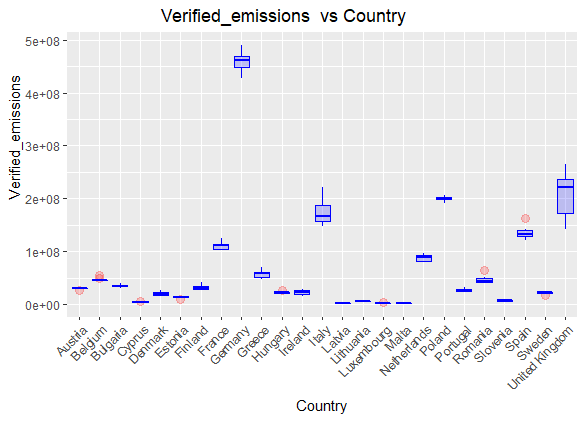
\includegraphics[width=1\linewidth]{images/Boxplot_Verified}
		\caption{}
		\label{fig:boxplot-Verified emissions-vs_country}
	\end{subfigure}
	\begin{subfigure}[]{0.8\textwidth}
		\centering
	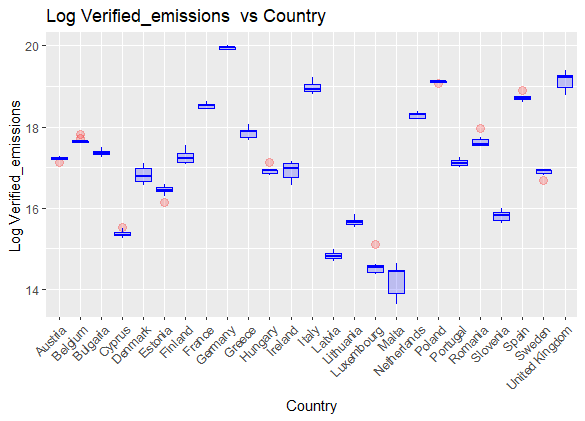
\includegraphics[width=1\linewidth]{images/boxplot_verified_log}
		\caption{}
		\label{fig:boxplot-Verified emissions_vs-country}
	\end{subfigure}
\end{figure}

\subsubsection{Agriculture}
	\begin{itemize}
	\item Source: http://wdi.worldbank.org/table/4.2
	\item Year:  2020
	\item Unit: Argicultural in Billions USD.
\end{itemize}  
\begin{table}[H]
	\centering
	\begin{tabular}{|r|rrrrr|r|}
  \hline
& min & 25-quantile & median & 75-quantile & max & Std \\ 
\hline
Austria & 4.32 & 4.79 & 5.14 & 5.46 & 6.05 & 0.55 \\ 
Belgium & 2.99 & 3.22 & 3.39 & 3.62 & 3.88 & 0.27 \\ 
Bulgaria & 2.04 & 2.20 & 2.39 & 2.56 & 3.20 & 0.33 \\ 
Cyprus & 0.37 & 0.44 & 0.49 & 0.52 & 0.59 & 0.07 \\ 
Denmark & 2.68 & 3.02 & 3.87 & 4.49 & 5.41 & 0.91 \\ \hline
Estonia & 0.49 & 0.63 & 0.65 & 0.80 & 0.85 & 0.13 \\ 
Finland & 5.29 & 5.82 & 6.03 & 6.41 & 6.59 & 0.43 \\ 
France & 35.54 & 39.60 & 42.43 & 44.42 & 47.28 & 3.91 \\ 
Germany & 22.99 & 25.78 & 29.91 & 32.78 & 35.20 & 4.54 \\ 
Greece & 6.79 & 7.71 & 8.33 & 8.85 & 9.99 & 0.90 \\ \hline
Hungary & 4.01 & 4.87 & 5.31 & 5.51 & 5.67 & 0.60 \\ 
Ireland & 1.32 & 2.28 & 2.61 & 3.06 & 3.96 & 0.71 \\ 
Italy & 36.20 & 38.32 & 40.70 & 43.21 & 45.94 & 3.17 \\ 
Latvia & 0.85 & 0.96 & 0.97 & 1.07 & 1.24 & 0.11 \\ 
Lithuania & 0.95 & 1.38 & 1.55 & 1.66 & 1.71 & 0.24 \\ \hline
Luxembourg & 0.13 & 0.14 & 0.15 & 0.17 & 0.20 & 0.02 \\ 
Malta & 0.09 & 0.10 & 0.11 & 0.11 & 0.13 & 0.01 \\ 
Netherlands & 13.20 & 13.89 & 15.07 & 15.49 & 15.71 & 0.92 \\ 
Poland & 11.25 & 13.13 & 14.22 & 15.96 & 16.76 & 1.91 \\ 
Portugal & 4.16 & 4.38 & 4.64 & 4.77 & 5.17 & 0.32 \\ \hline
Romania & 7.87 & 8.47 & 9.88 & 10.88 & 13.51 & 1.74 \\ 
Slovenia & 0.89 & 0.91 & 0.92 & 1.01 & 1.22 & 0.10 \\ 
Spain & 31.90 & 34.18 & 34.84 & 36.07 & 39.19 & 2.23 \\ 
Sweden & 6.27 & 7.53 & 8.11 & 8.47 & 9.59 & 0.87 \\ 
United Kingdom & 14.74 & 16.11 & 17.05 & 18.33 & 22.84 & 2.28 \\ 
\hline
	\end{tabular}
	\caption{Agriculture}
	\label{Agriculture}
\end{table}

\begin{figure}[H]
	\centering
	\begin{subfigure}[]{0.8\textwidth}
		\centering
		\includegraphics[width=1\linewidth]{images/Boxplot_Agriculture}
		\caption{}
		\label{fig:boxplot-Agriculture-vs-country}
	\end{subfigure}

\end{figure}

\newpage
\subsubsection{Industry}
	\begin{itemize}
	\item Source: http://wdi.worldbank.org/table/4.2
	\item Year:  2020
	\item Unit:  Industry in Billions USD
\end{itemize}  
\begin{table}[H]
	\centering
	\begin{tabular}{|r|rrrrr|r|}
  \hline
& min & 25-quantile & median & 75-quantile & max & Std \\ 
\hline
Austria & 96.16 & 102.24 & 106.03 & 111.06 & 116.48 & 6.50 \\ 
Belgium & 90.94 & 98.13 & 100.59 & 104.53 & 111.72 & 6.42 \\ 
Bulgaria & 12.04 & 13.16 & 13.62 & 14.01 & 14.87 & 0.87 \\ 
Cyprus & 2.03 & 2.45 & 2.95 & 3.63 & 4.98 & 0.90 \\ 
Denmark & 60.50 & 64.40 & 68.89 & 69.76 & 79.84 & 5.40 \\ \hline
Estonia & 4.61 & 5.63 & 5.97 & 6.42 & 7.36 & 0.81 \\ 
Finland & 54.66 & 61.38 & 63.49 & 65.70 & 84.47 & 7.78 \\ 
France & 431.14 & 459.74 & 479.72 & 506.08 & 551.30 & 36.97 \\ 
Germany & 843.80 & 934.68 & 1000.01 & 1014.25 & 1085.27 & 69.42 \\ 
Greece & 27.44 & 28.64 & 35.83 & 42.48 & 55.73 & 9.66 \\ \hline
Hungary & 32.23 & 32.95 & 33.99 & 36.13 & 40.79 & 2.98 \\ 
Ireland & 51.79 & 57.18 & 62.99 & 110.85 & 141.75 & 32.57 \\ 
Italy & 383.06 & 431.67 & 449.66 & 474.26 & 568.48 & 50.60 \\ 
Latvia & 4.90 & 5.37 & 5.81 & 6.01 & 7.81 & 0.78 \\ 
Lithuania & 9.38 & 11.12 & 12.22 & 13.05 & 13.97 & 1.52 \\ \hline
Luxembourg & 5.99 & 6.42 & 6.93 & 7.48 & 7.80 & 0.62 \\ 
Malta & 1.36 & 1.48 & 1.54 & 1.59 & 1.84 & 0.14 \\ 
Netherlands & 138.29 & 155.19 & 166.89 & 173.29 & 204.75 & 19.28 \\ 
Poland & 129.76 & 146.41 & 150.02 & 156.35 & 169.32 & 10.65 \\ 
Portugal & 38.81 & 41.82 & 43.54 & 47.46 & 53.70 & 4.42 \\ \hline
Romania & 54.81 & 61.02 & 63.42 & 67.76 & 78.81 & 7.80 \\ 
Slovenia & 12.08 & 12.77 & 13.77 & 13.95 & 16.62 & 1.31 \\ 
Spain & 240.11 & 268.98 & 278.66 & 328.16 & 429.02 & 57.54 \\ 
Sweden & 97.80 & 114.87 & 122.21 & 126.94 & 135.67 & 10.52 \\ 
United Kingdom & 448.57 & 473.78 & 494.10 & 522.75 & 583.44 & 40.55 \\ 
\hline
\end{tabular}
\caption{Industry}
\label{Industry}
\end{table}

\subsubsection{Manufacturing}
	\begin{itemize}
	\item Source: http://wdi.worldbank.org/table/4.2
	\item Year:  2020
	\item Unit:  Manufacturing in Billions USD.
\end{itemize} 

Εδώ φαίνεται εμφανώς πως έχω κάνει ένα τεράστιο λάθος. Λείπουν οι τιμές για το Manufacturing στην Βουλγαρία και νόμιζα πως το είχα βάλει να παίρνει έναν μέσο όρο και πως αυτό δεν θα άλλαζε σημαντικά τα αποτελέσματα. Όμως είναι εμφανές πως η Βουλγαρία όχι μόνο δεν έπαιρνε τις τιμές που ήθελα, αλλά και να συνέβαινε αυτό είναι πολύ πιθανό και πάλι να μην ήταν αρκετά λογικό το αποτέλεσμα. Η Βουλγαρία μάλλον θα πρέπει να αφαιρεθεί από τις δοκιμές, μαζί με χώρες όπως η Σλοβακία. 

\begin{table}[H]
	\centering
	\begin{tabular}{|r|rrrrr|r|}
  \hline
& min & 25-quantile & median & 75-quantile & max & Std \\ 
\hline
Austria & 63.75 & 66.61 & 70.28 & 72.47 & 76.57 & 4.24 \\ 
Belgium & 58.69 & 62.46 & 64.21 & 66.70 & 72.39 & 4.02 \\ 
Bulgaria & -470.74 & -453.31 & -432.37 & -420.07 & -399.33 & 22.79 \\ 
Cyprus & 0.85 & 0.95 & 1.12 & 1.33 & 1.52 & 0.23 \\ 
Denmark & 35.21 & 37.47 & 40.47 & 41.64 & 46.70 & 3.45 \\ \hline
Estonia & 2.41 & 3.20 & 3.35 & 3.56 & 4.13 & 0.47 \\ 
Finland & 34.44 & 38.11 & 39.73 & 42.29 & 59.40 & 6.76 \\ 
France & 254.30 & 268.11 & 278.31 & 292.38 & 325.40 & 20.87 \\ 
Germany & 603.23 & 697.07 & 743.97 & 755.59 & 796.43 & 56.32 \\ 
Greece & 15.64 & 16.78 & 18.19 & 22.95 & 30.27 & 4.63 \\ \hline
Hungary & 22.45 & 24.56 & 25.39 & 27.39 & 29.71 & 2.23 \\ 
Ireland & 43.26 & 47.00 & 49.10 & 100.06 & 126.39 & 31.76 \\ 
Italy & 264.39 & 290.81 & 301.69 & 308.97 & 372.63 & 28.24 \\ 
Latvia & 2.57 & 2.85 & 3.20 & 3.32 & 3.63 & 0.32 \\ 
Lithuania & 5.65 & 7.20 & 8.00 & 8.15 & 8.91 & 0.96 \\ \hline
Luxembourg & 2.53 & 2.88 & 3.14 & 3.41 & 3.93 & 0.42 \\ 
Malta & 0.83 & 0.96 & 1.00 & 1.06 & 1.23 & 0.11 \\ 
Netherlands & 82.70 & 89.39 & 91.54 & 95.12 & 109.07 & 7.43 \\ 
Poland & 71.81 & 82.05 & 85.70 & 88.28 & 98.64 & 7.14 \\ 
Portugal & 24.20 & 25.62 & 27.24 & 27.71 & 31.35 & 2.12 \\ \hline
Romania & 35.95 & 37.70 & 39.72 & 44.53 & 49.91 & 4.70 \\ 
Slovenia & 8.43 & 8.69 & 9.28 & 9.90 & 11.00 & 0.87 \\ 
Spain & 135.09 & 148.07 & 155.06 & 166.17 & 207.17 & 19.84 \\ 
Sweden & 60.02 & 69.65 & 72.99 & 77.49 & 83.80 & 6.77 \\ 
United Kingdom & 218.33 & 242.14 & 251.42 & 268.16 & 286.56 & 20.19 \\ 
\hline
	\end{tabular}
	\caption{Manufacturing}
	\label{Manufacturing}
\end{table}

\begin{figure}[H]
	\centering
	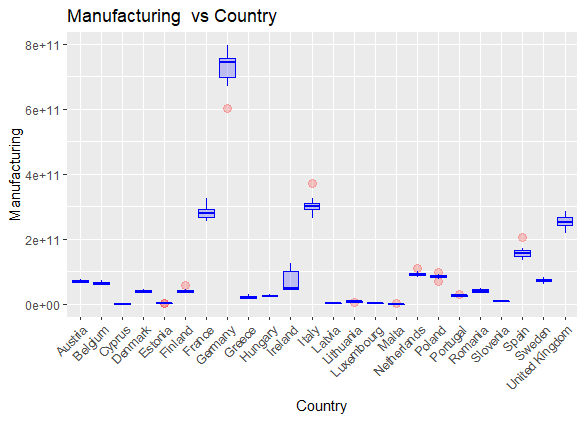
\includegraphics[width=0.5\linewidth]{images/boxplot_Manufacturing}
	\caption{}
	\label{fig:boxplotmanufacturing}
\end{figure}
\section{Για την 21η Μαρτίου}
Είχαμε πει, να βάλουμε κάποια πρόταση για δουλειά, ώστε να αρχίσει να ετοιμάζεται το paper. 
Αυτά που έπρεπε να κάνω εγώ είναι:
\begin{itemize}
	\item Να δούμε αν τα free ήταν το πρόβλημα για την πολωνία και την Γαλλία για το 2012 και το 2013.
	\item Να βρεθούν βάρη τα οποία να λειτουργούν για όλους καλά. Χωρίς να αλλάζουν κάθε φορά
	\item Διάβασμα για Nass Wellfare
	\item Να αναφερθούν ελλείψεις στα data
	\end {itemize}
	
	\subsection{Γιατί η Πολωνία και η Γαλλία αποτυγχάνουν να εξηγήσουν τις άλλες πριν το 2012;}
	Τελικά η απάντηση ήταν απίστευτα απλή. Κάτι πάει λάθος με τις δωρεάν άδειες, ή απλά έπαιρναν υπέρβολικά πολλές στην προηγούμενη φάση. όλες οι χώρες έχασαν πολλές δωρεάν άδειες από το 2012 στο 2013. Αλλά ας δούμε τι ποσοστό έχασαν και όλα θα βγάλουν νόημα. Spoiler, δεν βγάζει. Όχι μόνο δεν είναι παό τις πιο "ακραίες", αλλά μάλιστα είναι και σχετικά στην μέση.:


\begin{table}[H]
	\centering
	\begin{tabular}{|r|rrr|}
		\hline
		Country & 2012 free in Millions & 2013 free in Millions & Percentage drop in \% \\
		\hline
		 Malta & 2.37 & 0.18 & -92.52 \\
		 Cyprus & 6.70 & 1.15 & -82.89 \\ 
		 Estonia & 14.30 & 3.11 & -78.25 \\
		 Greece & 65.92 & 14.50 & -78.01 \\
		 Bulgaria & 43.08 & 10.68 & -75.22 \\\hline
		United Kingdom & 283.33 & 72.30 & -74.48 \\
		 Slovenia & 8.31 & 2.32 & -72.04 \\ 
		  \rowcolor{cyan} Poland & 213.47 & 63.63 & -70.20 \\
		 Luxembourg & 4.80 & 1.45 & -69.79 \\
		Romania & 75.61 & 24.06 & -68.18 \\\hline
	Portugal & 35.04 & 12.37 & -64.69 \\ 
		 Ireland & 28.76 & 10.54 & -63.36 \\
		 Germany & 467.32 & 173.23 & -62.93 \\
		 Spain & 163.59 & 67.11 & -58.98 \\
		 Italy & 197.62 & 87.81 & -55.56 \\\hline
		Hungary & 25.79 & 12.24 & -52.54 \\ 
		Denmark & 25.17 & 12.65 & -49.72 \\
		Netherlands & 99.37 & 50.24 & -49.44 \\
		 Latvia & 5.30 & 2.77 & -47.83 \\
		 \rowcolor[rgb]{1,0.5,0.5} France & 159.96 & 84.38 & -47.25 \\\hline
		 Finland & 40.28 & 23.05 & -42.77 \\
		 Belgium & 61.61 & 37.56 & -39.04 \\
		Austria & 35.38 & 22.88 & -35.33 \\
		 Lithuania & 8.43 & 6.55 & -22.33 \\ 
		 Sweden & 25.72 & 30.21 & 17.47 \\
		\hline
		\end{tabular}
	\end{table}

Άρα καμία απάντηση ακόμα...
\subsection{Τα βέλτιστα βάρη για όλα τα σενάρια}
Το πρώτο βήμα είναι λογικά να δοκιμαστούν τα πρώτα τα βάτη που προέκυψαν ως μέσος όρος όλων των βέλτιστων βαρών. Σε δεύτερο βήμα, πιθανότατα έχει νόημα να δοκιμάσουμε να μεγιστοποιήσουμε το γινόμενο όλων. 
	\begin{itemize}
	\item Population: 59.63
	\item GDP per capita: 19.85
	\item Inflation: 15.12
	\item Agriculture: 69.09
	\item Industry: 407.60
	\item Manufacturing: 12.69
	\item Total energy supply: 170.25
	\item Verified emissions: 849.81\\
\end{itemize}
\begin{table}[ht]
	\centering
			\tabcolsep=0.11cm
	\begin{tabular}{|r|rrrrr|rrrrrr|rr|}
		\hline
		& 2008 & 2009 & 2010 & 2011 & 2012 & 2013 & 2014 & 2015 & 2016 & 2017 & 2018 & max p-value & max MSE \\ 
		\hline
		Austria & 0.94 & 0.93 & 0.94 & 0.94 & 0.95 & 0.97 & 0.97 & 0.97 & 0.96 & 0.95 & 0.95 & 0.00 & 0.00 \\
		Belgium & 0.91 & 0.90 & 0.93 & 0.93 & 0.93 & 0.86 & 0.83 & 0.82 & 0.80 & 0.78 & 0.78 & 0.00 & 0.00 \\ 
		Bulgaria & 0.92 & 0.91 & 0.93 & 0.92 & 0.94 & 0.96 & 0.96 & 0.97 & 0.95 & 0.96 & 0.96 & 0.00 & 0.00 \\
		Cyprus & 0.95 & 0.94 & 0.94 & 0.95 & 0.96 & 0.95 & 0.94 & 0.96 & 0.96 & 0.96 & 0.96 & 0.00 & 0.00 \\ 
		Denmark & 0.95 & 0.94 & 0.93 & 0.94 & 0.96 & 0.96 & 0.96 & 0.96 & 0.96 & 0.95 & 0.95 & 0.00 & 0.00 \\		\hline
		Estonia & 0.94 & 0.94 & 0.94 & 0.94 & 0.95 & 0.94 & 0.95 & 0.96 & 0.95 & 0.96 & 0.96 & 0.00 & 0.00 \\
		Finland & 0.94 & 0.93 & 0.94 & 0.94 & 0.95 & 0.96 & 0.97 & 0.96 & 0.97 & 0.96 & 0.95 & 0.00 & 0.00 \\ 
		France & 0.58 & 0.53 & 0.73 & 0.77 & 0.83 & 0.90 & 0.86 & 0.85 & 0.85 & 0.90 & 0.89 & 0.00 & 0.01 \\
		Germany & 0.92 & 0.92 & 0.93 & 0.94 & 0.95 & 0.97 & 0.96 & 0.95 & 0.95 & 0.94 & 0.93 & 0.00 & 0.00 \\
		Greece & 0.87 & 0.88 & 0.89 & 0.89 & 0.91 & 0.94 & 0.94 & 0.96 & 0.97 & 0.96 & 0.96 & 0.00 & 0.00 \\ 		\hline
		Hungary & 0.94 & 0.92 & 0.93 & 0.94 & 0.95 & 0.96 & 0.95 & 0.97 & 0.96 & 0.96 & 0.96 & 0.00 & 0.00 \\
		Ireland & 0.95 & 0.94 & 0.93 & 0.95 & 0.95 & 0.96 & 0.96 & 0.95 & 0.95 & 0.94 & 0.94 & 0.00 & 0.00 \\
		Italy & 0.83 & 0.80 & 0.87 & 0.91 & 0.93 & 0.88 & 0.90 & 0.94 & 0.94 & 0.94 & 0.93 & 0.00 & 0.00 \\ 
		Latvia & 0.94 & 0.94 & 0.94 & 0.94 & 0.95 & 0.96 & 0.96 & 0.96 & 0.96 & 0.97 & 0.96 & 0.00 & 0.00 \\
		Lithuania & 0.94 & 0.94 & 0.94 & 0.94 & 0.95 & 0.97 & 0.97 & 0.97 & 0.97 & 0.97 & 0.96 & 0.00 & 0.00 \\
		Luxembourg & 0.94 & 0.93 & 0.93 & 0.94 & 0.95 & 0.94 & 0.94 & 0.95 & 0.94 & 0.95 & 0.95 & 0.00 & 0.00 \\		\hline
		Malta & 0.94 & 0.93 & 0.94 & 0.94 & 0.96 & 0.96 & 0.96 & 0.96 & 0.96 & 0.97 & 0.96 & 0.00 & 0.00 \\ 
		Netherlands & 0.88 & 0.87 & 0.88 & 0.86 & 0.88 & 0.76 & 0.74 & 0.71 & 0.72 & 0.67 & 0.62 & 0.00 & 0.01 \\
		Poland & 0.19 & 0.21 & 0.28 & 0.35 & 0.45 & 0.81 & 0.86 & 0.89 & 0.93 & 0.93 & 0.92 & 0.04 & 0.01 \\
		Portugal & 0.94 & 0.93 & 0.94 & 0.94 & 0.95 & 0.96 & 0.97 & 0.97 & 0.96 & 0.96 & 0.96 & 0.00 & 0.00 \\
		Romania & 0.84 & 0.82 & 0.83 & 0.86 & 0.87 & 0.96 & 0.98 & 0.98 & 0.96 & 0.95 & 0.96 & 0.00 & 0.00 \\ 
		Slovenia & 0.95 & 0.93 & 0.93 & 0.94 & 0.95 & 0.96 & 0.96 & 0.96 & 0.96 & 0.96 & 0.96 & 0.00 & 0.00 \\		\hline
		Spain & 0.93 & 0.92 & 0.89 & 0.88 & 0.90 & 0.80 & 0.87 & 0.90 & 0.88 & 0.92 & 0.90 & 0.00 & 0.00 \\
		Sweden & 0.94 & 0.93 & 0.93 & 0.93 & 0.94 & 0.94 & 0.94 & 0.94 & 0.94 & 0.93 & 0.93 & 0.00 & 0.00 \\
		United Kingdom & 0.92 & 0.94 & 0.95 & 0.94 & 0.94 & 0.84 & 0.89 & 0.89 & 0.96 & 0.94 & 0.94 & 0.00 & 0.00 \\ 
		\hline
	\end{tabular}
\end{table}
Εδώ πλέον γίνεται πολύ αμφισβητήσιμο το αν χρειάζεται να ψάξουμε για κάτι καλύτερο. Με εξαίρεση την Πολωνία και την Γαλλία, οι υπόλοιποι δείχνουν να τα πηγαίνουν πολύ καλά. 

\section{Για την 28η Μαρτίου}
Είπαμε να γίνουν τα παρακάτω:
\begin{itemize}
	\item Να δούμε αν η Πολωνία είναι τόσο ανώμαλη, εξαιτίας του κανόνα 10c.
	\item Να προστεθούν στα features ξεχωριστά η πράσινη ενέργεια και ξεχωριστά η υπόλοιπη ενέργεια. 
	\item Να οριστεί και να προσομοιωθεί το παρακάτω πρόβλημα:
	\begin{itemize}
		\item max $\sum{u_i(x_i)*GDP_i}$
		\item $\sum {x_i} \leq$ Cap.
		\item Όπου $x_i$ είναι το allocation στην χώρα i.
		\item Η $u_i$ είναι ξεχωριστή για κάθε χώρα και δηλώνει την ικανοποίηση που λαμβάνει η αντίστοιχη χώρα με το αντίστοιχο allocation.
	\end{itemize}
	\item Πιθανότατα η  $u_i$ θα μπορούσε να είναι το energy intensity.
	\item Μετά μπορούν να προστεθούν επιπλέον constrains 
	\item Να προστεθεί το energy Intensity στα features της κάθε χώρας.
\end{itemize}


\subsection{Τι όντως έκανα}
\begin{itemize}
	\item Δεν υλοποίησα κανένα κομμάτι του κώδικά. 
	\item Το power intensity δεν είναι απλώς μία τιμή. 
\end{itemize}
\subsection{PPS (Purchasing Power Standards)}
To PPS είναι ένα εικκονικό νόμισμα. Το οποίο προσπαθεί να πετύχει να είναι αποπληθωρισμένο, ενώ ταυτόχρονα προσπαθεί να αφαιρέσει διαφορές λόγω άλλης αγοραστικής δύναμης.
\subsubsection{Χρήση PPS}
To PPS χρησιμοποιείται προκειμένου να κάνουμε συγκρείσεις μεταξύ διαφορετικών χωρών. Το βρίσκουμε συνήθως στα dataset της eurostat ως MPPS (Million Purchasing Power Standarts).
\subsubsection{Υπολογισμός}
Ένα PPS ισοδυναμεί με ένα καλάθι στην εκάστοτε χώρα. Το καλάθι αυτό έχει ένα μείγμα από διάφορα προϊόντα και υπηρεσίες. Το κόστων αυτών συμπεριλαμβωάνεται σε έναν σταθμισμένο μέσο, εκ του οποίου προκύπτει μία τιμή, η οποία είναι το κόστος του καλαθιού. Στην συνέχεια, μπορούμε να χρησιμοποιήσουμε αυτήν την τιμή για να κανονικοποιήσουμε διαφορετικές "αξίες" μεταξύ διαφορετικών χωρών ώστε να μπορούμε να κάνουμε συγκρίσεις με βάση την αγοραστική δύναμη και όχι απλά ευρώ. 
\subsection{Power Intensity}

Energy intensity can be considered as an approximation of the energy efficiency of a country’s economy, and shows the amount of energy needed to produce a unit of GDP. There are various reasons for observed improvements in energy intensity: a general shift from industry towards a service-based economy in Europe, a shift within industry to less energy-intensive activities and production methods, the closure of inefficient units, and more energy-efficient appliances.


To Power Intensoty υπολογίζεται ως $$Power\_Instenstity = \frac{Units\_of\_Energy}{Units\_of\_GDP}$$
Αυτό λοιπόν μπορούμε να το υπολογίσουμε με δύο διαφορετικούς τρόπους. 
\begin{itemize}
	\item Chain Linked Volumes. Χρησιμοποιείται για να κάνουμε συγκερίσεις για μία χώρα σε βάθος χρόνου. Εδώ είναι σημαντικό το να σημειωθεί πως είναι πιθανό να μην αρκεί μία τιμή για να κάνουμε την δουλειά μας. Οι τιμές προκύπτουν σε επίπεδο έτους. Όμως οι οικονομικές αλλαγές στις χώρες (όπως αλλαγές σε φορολογίες) δημιουργούν μεγάλες ανωμαλίες στα δεδομένα, επομένως είναι καλύτερο να χρησιμοποιούνται περισσότερα από 4 data points.
	
	\item Η άλλη επιλογή είναι το να χρησιμοποιήσουμε τα δεςδομένα σε PPS,  αυτή η επιλογή μας επιτρέπει να βγάλουμε συμπεράσματα μεταξύ χωρών. 
\end{itemize}

\subsection{Για την επόμενη φορά}
\subsubsection{Σε δεύτερo χρόνο}
\begin{itemize}
	\item Ορίζουμε ένα πρόβλημα βελτιστοποίησης. Χρησιμοποιούμε το power instensity ως το εργαλείο το οποίο θα μας εξηγεί ποια χώρα είναι σε θέση να διαχειρσιτεί με πιο αποτελεσματικό τρόπου τους ρίπους. Μας ενδιαφέρει το power intensity όπως αυτό βρίσκεται στην eurostat στο NRG\_IND\_EI, από όπου θα αναζητήσουμε την έτοιμη τιμή PPS.
	
	Στην συνέχεια θα υλοποιηθούν τα παρακάτω:
	\begin{itemize}
		\item Vanila version. Θα είναι λογικά ίδιο με αυτό που είχαμε κάνει στο παρελθόν, μόνο που εκεί αντί για το power intensity είχαμε τον λόγo $\frac{GDP}{verified}$.
		\item Διάφορα constrains και συνδυασμοί αυτών. 
		\item Να πλησιάσουμε να βρούμε συνδυασμό από περιορισμούς οι οποίοι να προσεγγίζει τις τιμές που προκύπτουν από το EU ETS.
		
	\end{itemize}
\item Διάβασμα το "Cap and Trade and Emission Clustering : A spatial-temporal analysis of the EU ETSheme".
\end{itemize}
Ορίζουμε ένα πρόβλημα βελτιστοποίησης. Χρησιμοποιούμε το power instensity ως το εργαλείο το οποίο θα μας εξηγεί ποια χώρα είναι σε θέση να διαχειρσιτεί με πιο αποτελεσματικό τρόπου τους ρίπους. Μας ενδιαφέρει το power intensity όπως αυτό βρίσκεται στην eurostat στο NRG\_IND\_EI, από όπου θα αναζητήσουμε την έτοιμη τιμή PPS.

Στην συνέχεια θα υλοποιηθούν τα παρακάτω:
\begin{itemize}
	\item Vanila version. Θα είναι λογικά ίδιο με αυτό που είχαμε κάνει στο παρελθόν, μόνο που εκεί αντί για το power intensity είχαμε τον λόγo $\frac{GDP}{verified}$.
	\item Διάφορα constrains και συνδυασμοί αυτών. 
	\item Να πλησιάσουμε να βρούμε συνδυασμό από περιορισμούς οι οποίοι να προσεγγίζει τις τιμές που προκύπτουν από το EU ETS.
	
\end{itemize}

\subsubsection{Άμεσα, για το τετρασέλιδο}
Για κάθε χώρα έχουμε έναν συνδυασμό από  features. Με βάση αυτά τα δεδομένα μπορούμε να τις ομαδοποιήσουμε σε 3 ή 4 κατηγορίες οι οποίες θα έχουν κοινά χαρακτηριστικά. Ύστερα, να απαντηθούν τα παρακάτω ερωτήματα:
\begin{itemize}
	\item Να προστεθούν και άλλα features για τις χώρες αυτές, όπως είναι το power intensity, το ποσοστό της πράσινης ενέργειας που παράγουν.
	\item Οι χώρες οι οποίες είμαι μέσα στο ίδιο cluster μπορούν να εξηγήσουν καλά τις υπόλοιπες του cluster τους;
	\item Μήπως χώρες διαφορετικών χωρών μπορούν να εξηγήσουν καλύτερη η μία την άλλη; (Υπόθεση Κώστα, μπορεί να ελεγχθεί τρέχοντας το ίδιο πρόβλημα, αλλά αφιαρώντας όλες τις άλλες χώρες του ίδιου cluster)
	\item Αν πάρω την χώρα που δρα ως κέντρο σε κάθε cluster τι προκύπτει;
	\item Μήπως μέσα στο ίδιο cluster παρατηρείται κάποια απλή σχέση των free με κάποιον από τα features ή με κάποιο συνδυασμό αυτών; 
\end{itemize}
\section{Για τις 4 Απριλίου}
Καλό μήνα!
\subsection{Συσταδοποίηση (έπρεπε...)}
\subsubsection{Πλήθος συστάδων}
	Στην R υπάρχει ένα πολύ όμορφο εργαλείο το οποίο προτείνει τον αριθμό των βέλτιστων clusters με 30 διαφορετικούς δείκτες (elbow, silouette κλπ).
	Με βάση τα δεδομένα μας, νομίζω πως οι 3 συστάδες είναι η βέλτιστη λύση.\\
	* Among all indices:\\
	* 6 proposed 2 as the best number of clusters\\
	* 9 proposed 3 as the best number of clusters\\
	* 1 proposed 4 as the best number of clusters \\
	* 1 proposed 5 as the best number of clusters\\
	* 5 proposed 9 as the best number of clusters\\
	* 2 proposed 10 as the best number of clusters\\
	
	***** Conclusion *****\\
	
	* According to the majority rule, the best number of clusters is  3
	Συγκεκριμένα, για όλες τις διαφορετικές μεθόδους προκύπτουν τα παρακάτω:
\begin{table}[ht]
	\centering
	\tabcolsep=0.11cm
	\begin{tabular}{|r|rrrr|rrrrr|rrrr|}
		\hline
		Clusters& KL & CH & Hartigan & CCC & Scott & Marriot & TrCovW & TraceW & Friedman & Rubin & Cindex & DB & Silhouette \\
		\hline
		2 & 4.16 & 30.55 & 10.06 & 5.49 & 140.15 & 0.00 & 0.91 & 5.56 & 221.35 & 4.54 & 0.35 & 0.76 & 0.56 \\
		\rowcolor[rgb]{0.9,0.9,0.9} 3 & 6.73 & 25.81 & 2.74 & 5.51 & 191.04 & 0.00 & 0.30 & 3.87 & 252.61 & 6.53 & 0.27 & 0.90 & 0.41 \\
		4 & 0.13 & 19.34 & 13.76 & 4.39 & 219.59 & 0.00 & 0.25 & 3.44 & 276.56 & 7.34 & 0.26 & 1.27 & 0.31 \\ 
		5 & 4.75 & 26.15 & 3.77 & 6.65 & 303.07 & 0.00 & 0.12 & 2.08 & 590.66 & 12.16 & 0.33 & 0.83 & 0.35 \\
		6 & 3.09 & 24.33 & 1.65 & 6.22 & 370.12 & 0.00 & 0.09 & 1.75 & 1,054.45 & 14.45 & 0.30 & 0.70 & 0.40 \\ 
		7 & 0.16 & 21.14 & 7.77 & 5.22 & 383.36 & 0.00 & 0.08 & 1.61 & 1,044.11 & 15.70 & 0.30 & 0.79 & 0.34 \\
		8 & 1.56 & 25.54 & 6.22 & 6.54 & 459.86 & 0.00 & 0.03 & 1.12 & 1,440.67 & 22.48 & 0.24 & 0.82 & 0.32 \\
		9 & 3.17 & 29.46 & 2.31 & 7.46 & 587.08 & 0.00 & 0.02 & 0.82 & 3,137.27 & 30.71 & 0.20 & 0.70 & 0.42 \\ 
		10 & 5.57 & 28.34 & 0.68 & 6.99 & 613.29 & 0.00 & 0.02 & 0.72 & 3,743.78 & 35.14 & 0.19 & 0.71 & 0.38 \\
		\hline
	\end{tabular}
\end{table}
\begin{table}[ht]
	\centering
	\tabcolsep=0.11cm
	\begin{tabular}{|r|rrrr|rrrrr|rrrr|}
		\hline
		Clusters& Duda & Pseudot2 & Beale & Ratkowsky & Ball & Ptbiserial & Frey & McClain & Dunn & Hubert & SDindex & Dindex & SDbw \\
		\hline
		2 & 0.56 & 14.33 & 3.99 & 0.47 & 2.78 & 0.76 & 2.96 & 0.20 & 0.40 & 0.16 & 8.57 & 0.42 & 0.64 \\ 
		\rowcolor[rgb]{0.9,0.9,0.9} 3 & 0.74 & 4.29 & 1.74 & 0.46 & 1.29 & 0.59 & 6.15 & 0.66 & 0.14 & 0.16 & 8.25 & 0.33 & 0.45 \\
		4 & 0.63 & 2.99 & 2.37 & 0.42 & 0.86 & 0.43 & -0.07 & 1.53 & 0.14 & 0.16 & 10.58 & 0.31 & 0.54 \\
		5 & 2.03 & -3.05 & -2.30 & 0.41 & 0.42 & 0.46 & 0.36 & 1.46 & 0.21 & 0.18 & 8.82 & 0.25 & 0.21 \\ 
		6 & 1.03 & -0.17 & -0.13 & 0.38 & 0.29 & 0.46 & 14.61 & 1.58 & 0.21 & 0.19 & 9.19 & 0.22 & 0.15 \\
		7 & 0.35 & 14.73 & 7.30 & 0.36 & 0.23 & 0.41 & 0.10 & 2.04 & 0.14 & 0.19 & 9.54 & 0.21 & 0.15 \\
		8 & 3.69 & -3.64 & -2.57 & 0.34 & 0.14 & 0.41 & 0.35 & 2.04 & 0.21 & 0.20 & 9.06 & 0.18 & 0.13 \\
		9 & 5.57 & -3.28 & -0.00 & 0.32 & 0.09 & 0.39 & 1.45 & 2.27 & 0.32 & 0.21 & 11.70 & 0.15 & 0.08 \\ 
		10 & 5.93 & -1.66 & -2.93 & 0.31 & 0.07 & 0.36 & -1.40 & 2.77 & 0.25 & 0.21 & 11.91 & 0.14 & 0.07 \\
		\hline
	\end{tabular}
\end{table}

\subsubsection{Βέλτιστες συστάδες}

\begin{figure}[H]
\centering
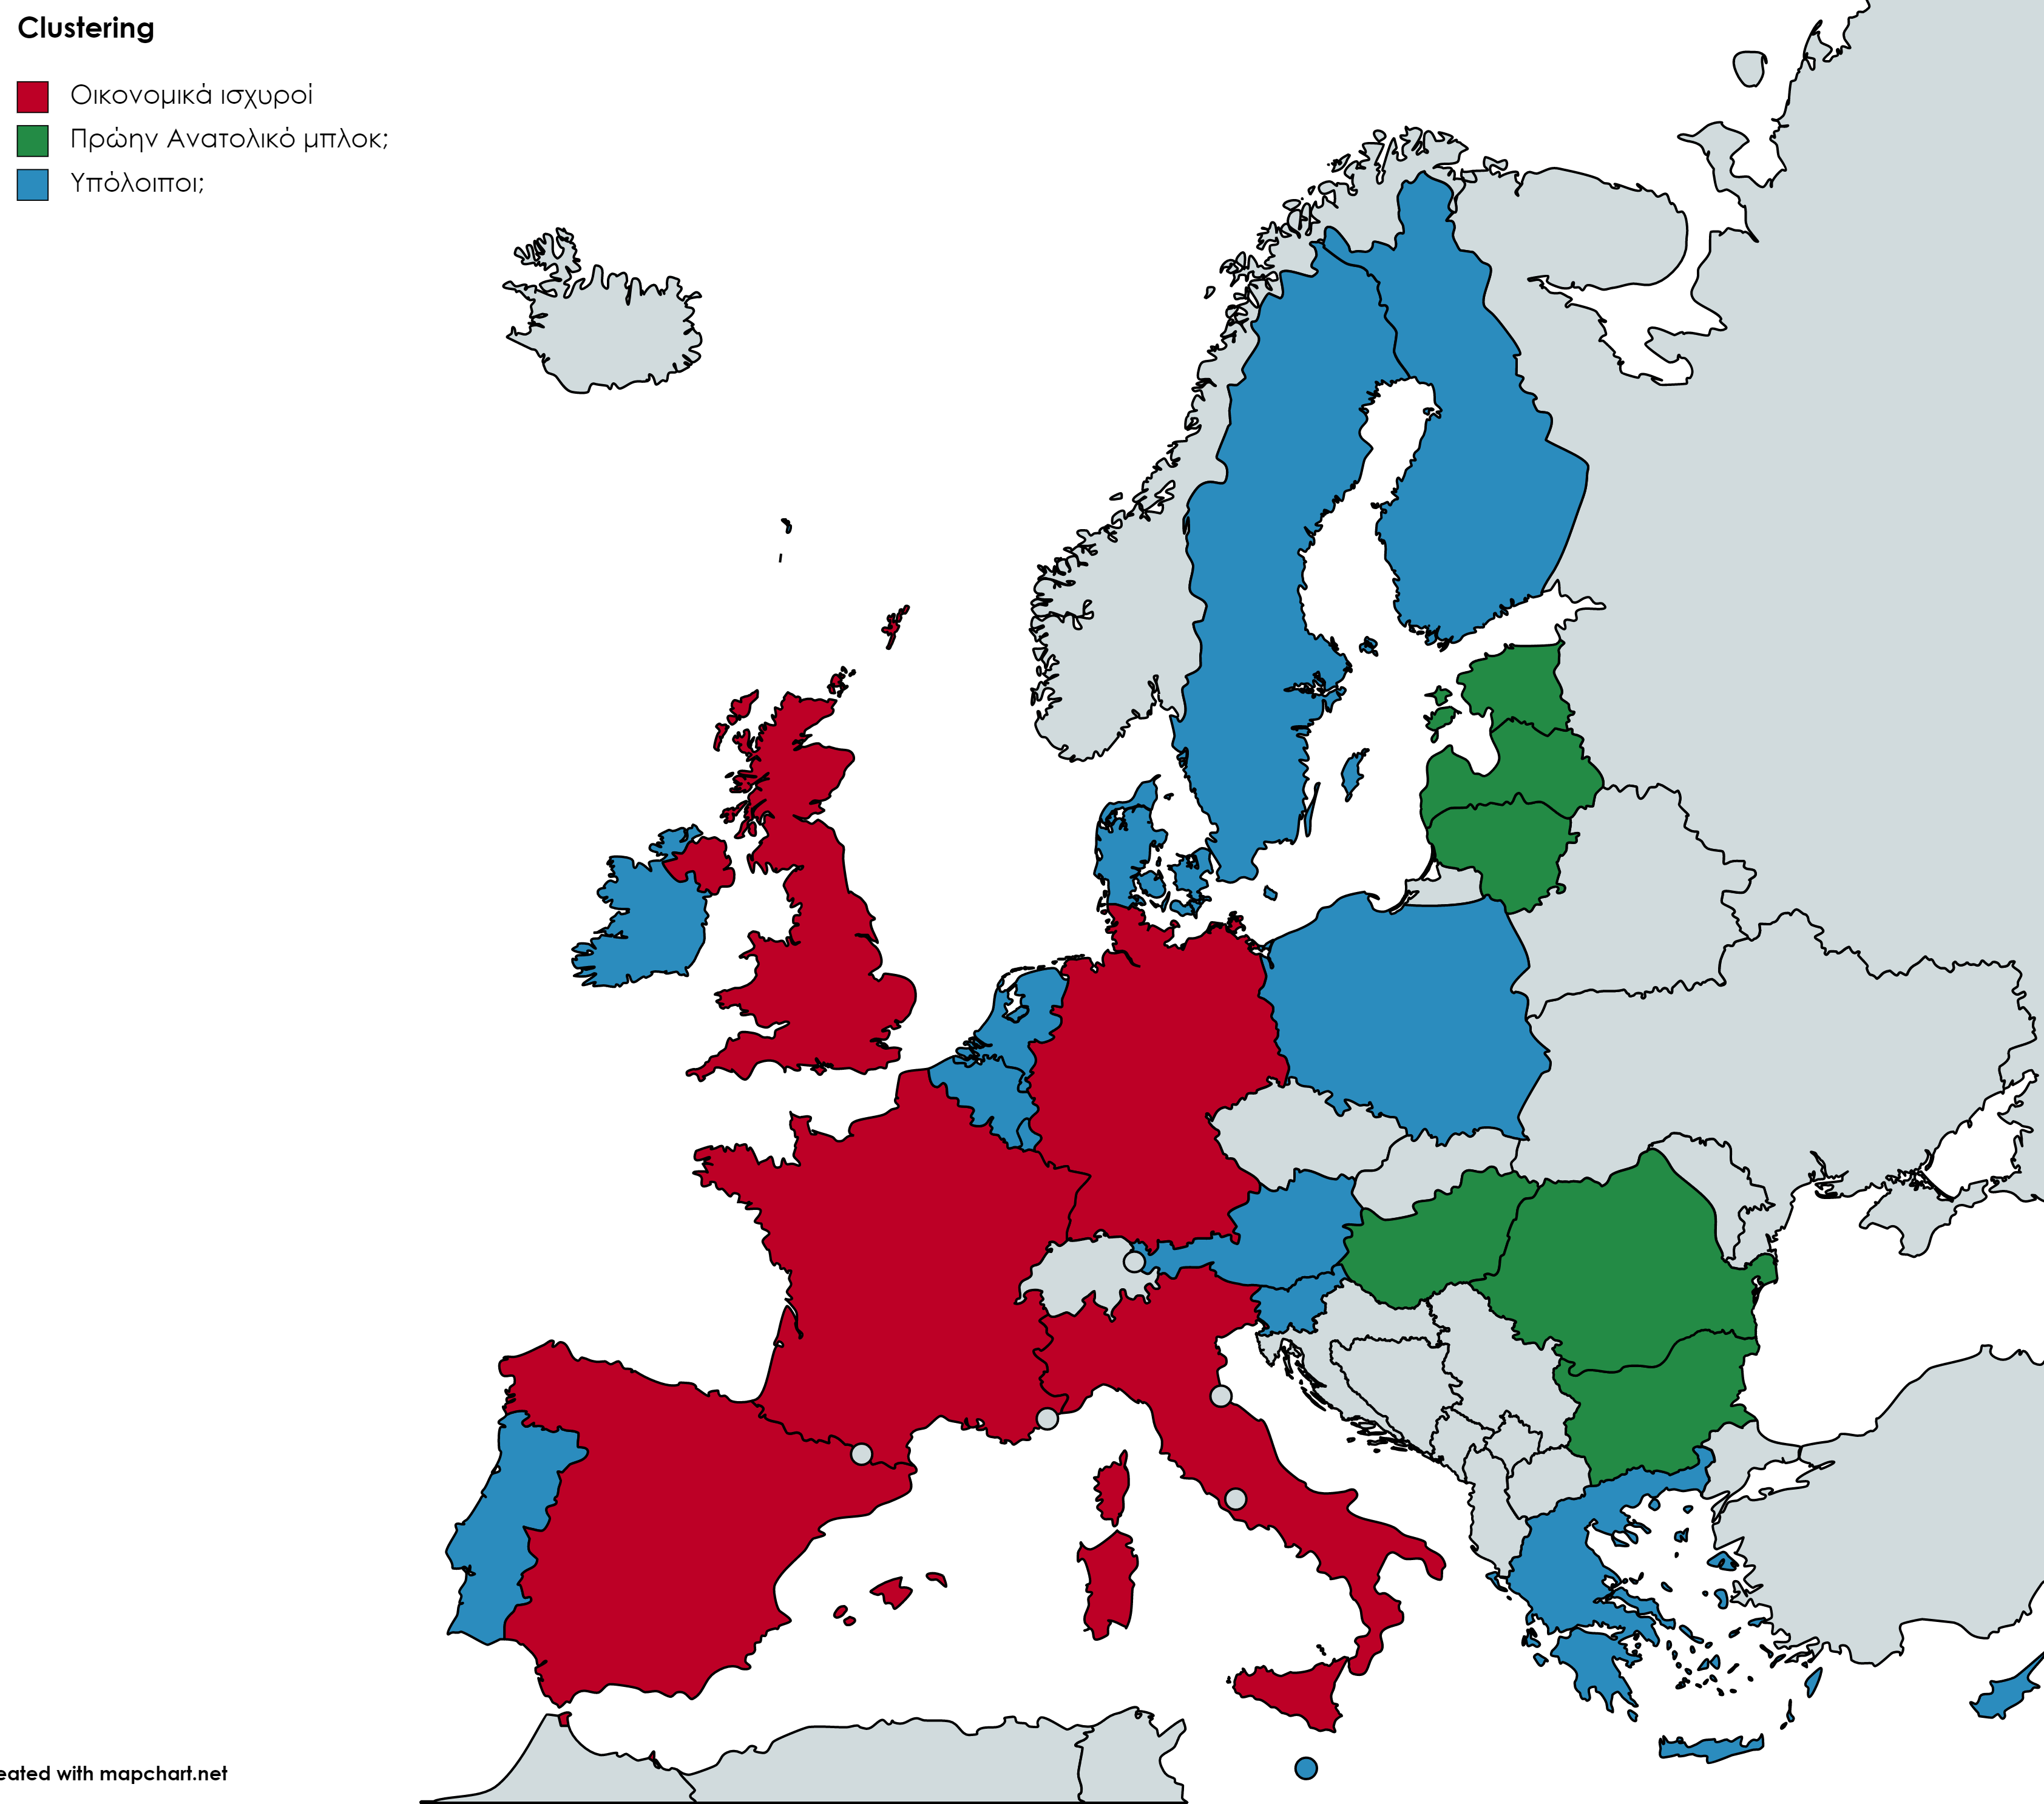
\includegraphics[width=0.65\linewidth]{images/Clustering}
\qquad
\begin{tabular}[b]{|cc|}
		\hline
Χώρα & partition \\
\hline
\rowcolor[rgb]{0.9,0.9,1} France &   1 \\
\rowcolor[rgb]{0.9,0.9,1}Germany &   1 \\
\rowcolor[rgb]{0.9,0.9,1}Italy &   1 \\
\rowcolor[rgb]{0.9,0.9,1}Spain &   1 \\ 
United Kingdom &   1 \\ \hline
Bulgaria &   2 \\
\rowcolor[rgb]{0.9,0.9,1}Estonia &   2 \\
Hungary &   2 \\
\rowcolor[rgb]{0.9,0.9,1}Latvia &   2 \\
\rowcolor[rgb]{0.9,0.9,1}Lithuania &   2 \\
Romania &   2 \\ \hline \hline
\rowcolor[rgb]{0.9,0.9,1}Austria &   3 \\
\rowcolor[rgb]{0.9,0.9,1}Belgium &   3 \\
\rowcolor[rgb]{0.9,0.9,1}Cyprus &   3 \\
Denmark &   3 \\
\rowcolor[rgb]{0.9,0.9,1}Finland &   3 \\
\rowcolor[rgb]{0.9,0.9,1}Greece &   3 \\ 
\rowcolor[rgb]{0.9,0.9,1}Ireland &   3 \\
\rowcolor[rgb]{0.9,0.9,1}Luxembourg &   3 \\
Malta &   3 \\
\rowcolor[rgb]{0.9,0.9,1}Netherlands &   3 \\
Poland &   3 \\
\rowcolor[rgb]{0.9,0.9,1}Portugal &   3 \\
\rowcolor[rgb]{0.9,0.9,1}Slovenia &   3 \\
Sweden &   3 \\
\hline
\rowcolor[rgb]{0.9,0.9,1} EUROZONE &\\
\hline
\end{tabular}
\captionlistentry[table]{A table beside a figure}
\caption{Συστάδες}
\end{figure}
Είναι λοιπόν σαν να εχουμε 3 βασικές κατηγορίες και σε αυτό ίσως φταίνε τα δεδομένα τα οποία έχω χρησιμοποιήσει. Μοιάζει σαν να είναι:
\begin{itemize}
	\item Εκβιομηχανισμένες χώρες
	\item Μέρος του ανατολικού μπλοκ
	\item Υπόλοιποι
\end{itemize}
\subsubsection{Συστάδες, αν όλα τα δεδομένα ήταν κατά κεφαλήν και κανονικοποιημένα ύστερα}
Αυτό δεν είχαμε πει να γίνει, όμως ένοιωσα την ανάγκη να το δοκιμάσω.

\begin{figure}[!ht]
	\centering
	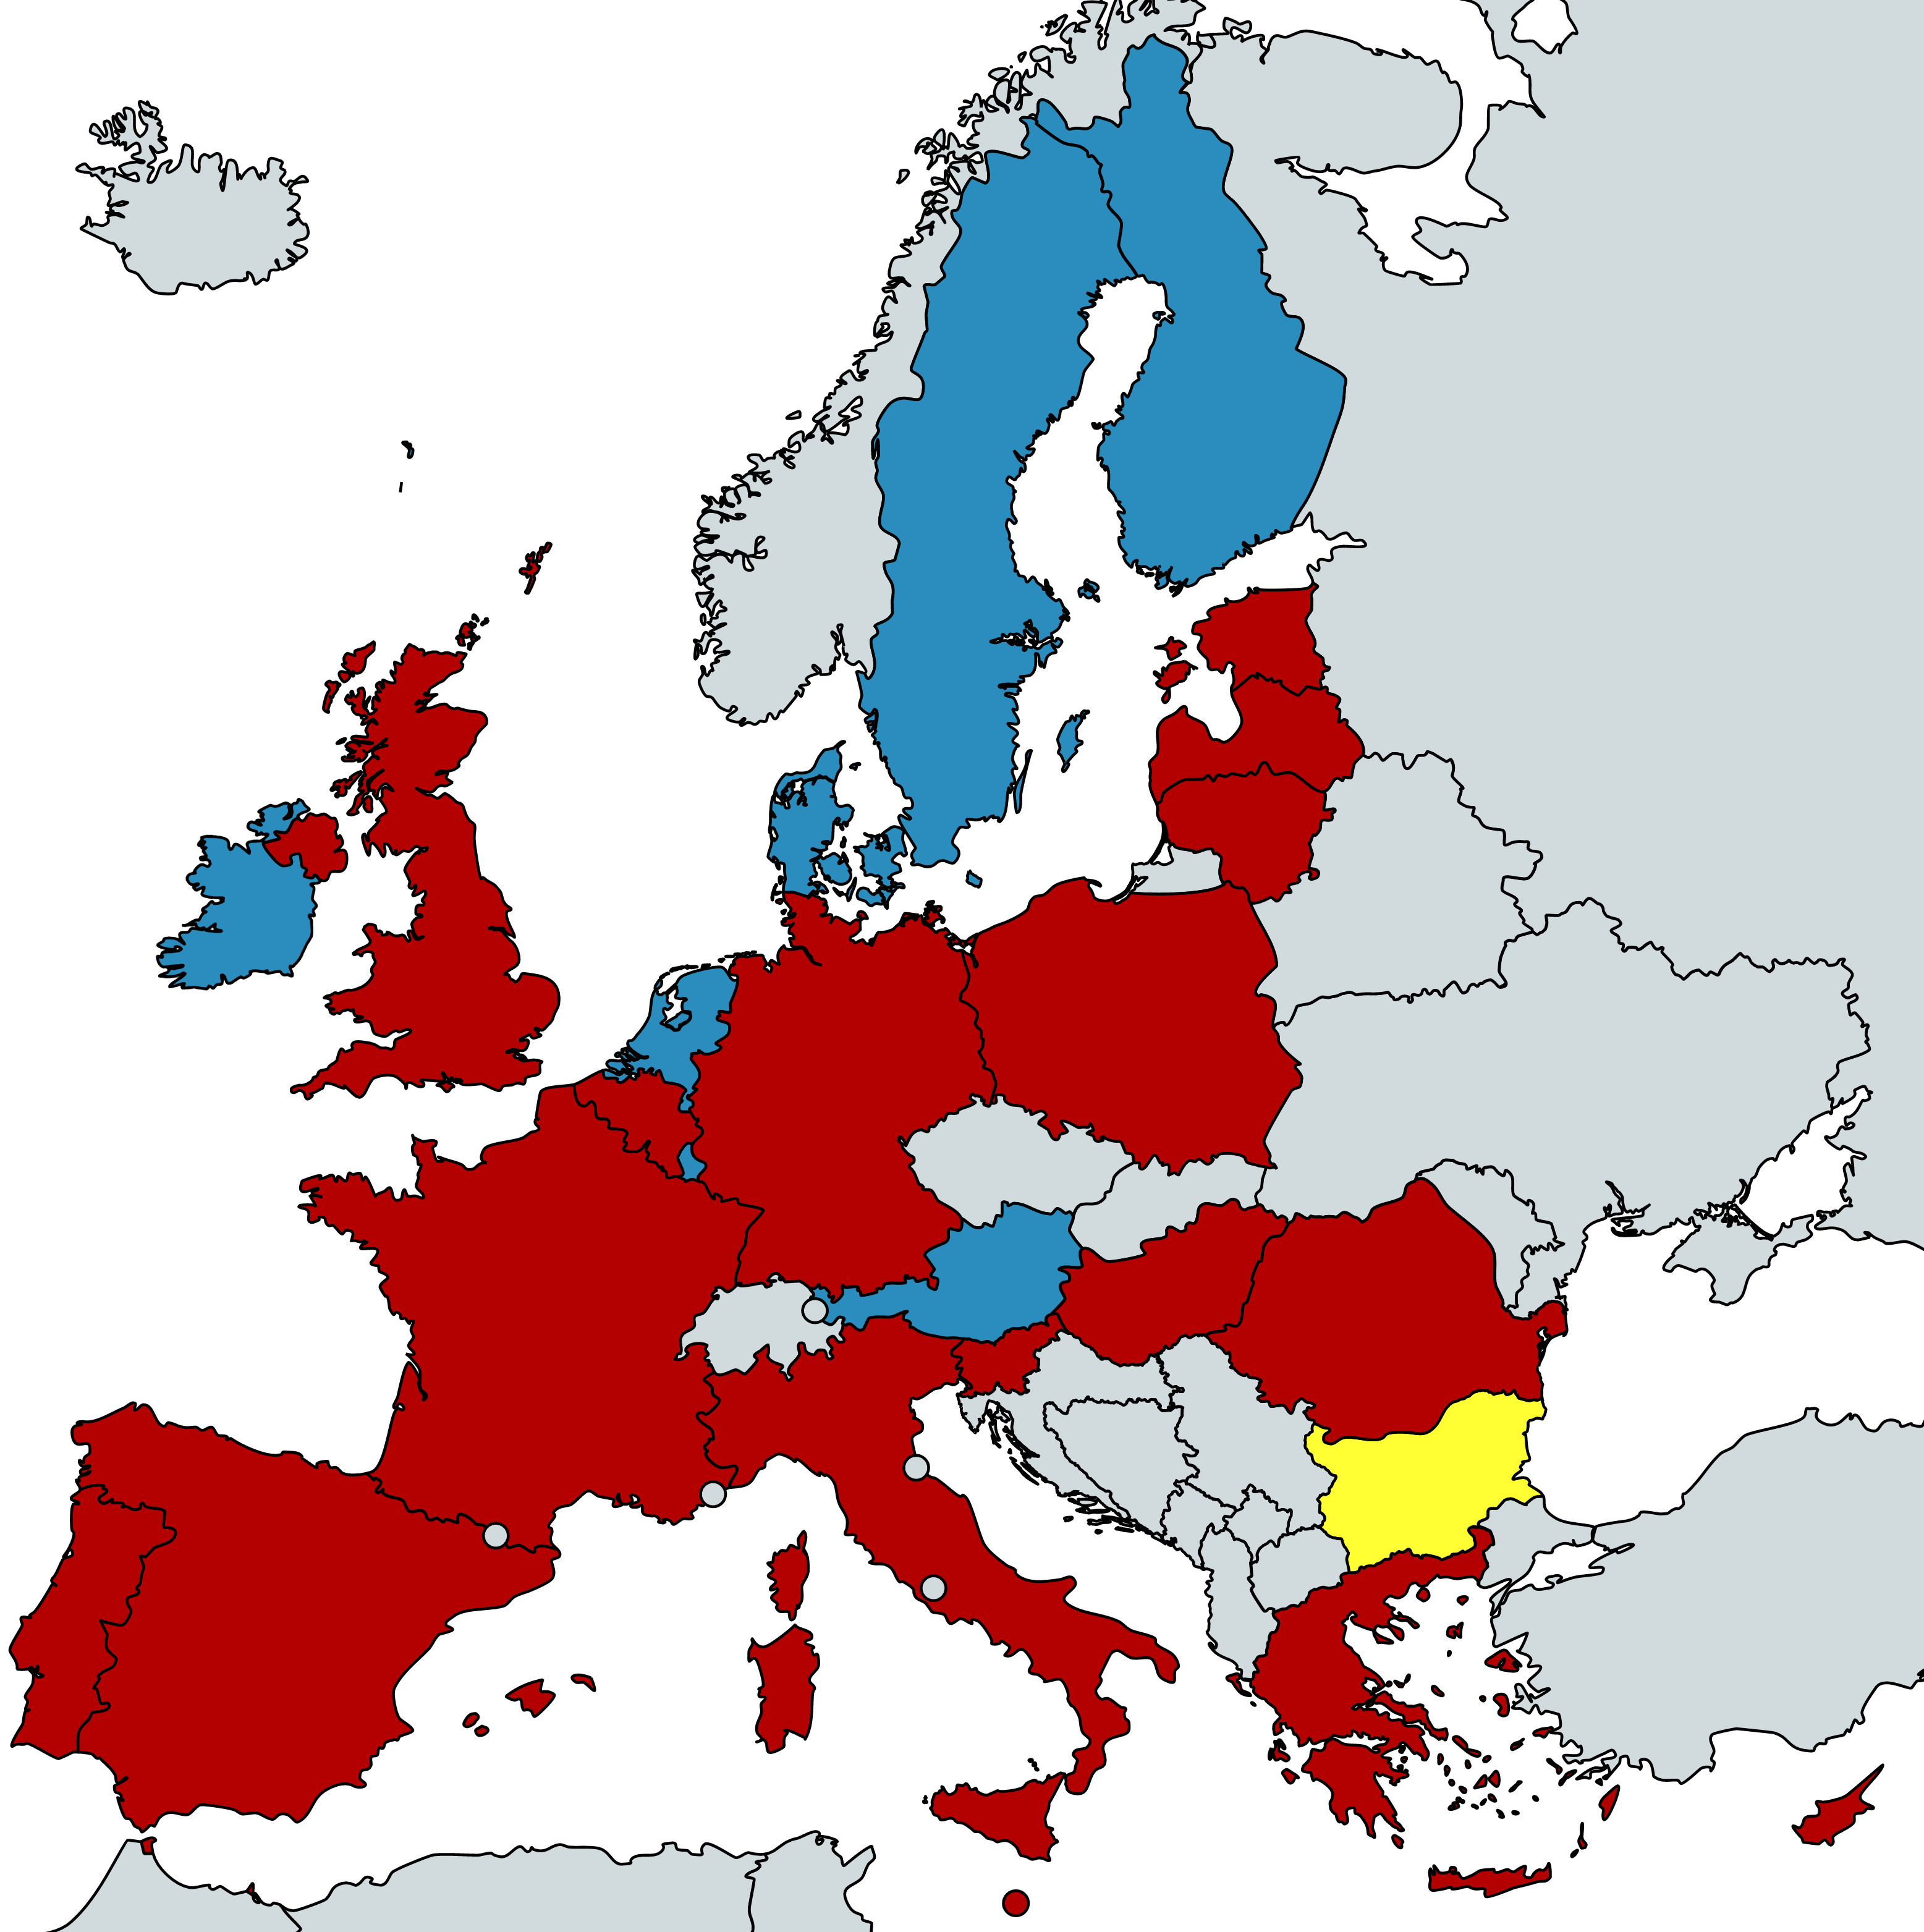
\includegraphics[width=0.65\linewidth]{images/Clustering_per_capita}
	\qquad
	\begin{tabular}[b]{|cc|}
		\hline
GEO & partition \\
\hline
Austria &   1 \\
Denmark &   1 \\ 
Finland &   1 \\
Ireland &   1 \\
Luxembourg &   1 \\
Netherlands &   1 \\
Sweden &   1 \\ \hline
Belgium &   2 \\
Cyprus &   2 \\
Estonia &   2 \\ 
France &   2 \\
Germany &   2 \\
Greece &   2 \\
Hungary &   2 \\
Italy &   2 \\
Latvia &   2 \\
Lithuania &   2 \\
Malta &   2 \\
Poland &   2 \\
Portugal &   2 \\ 
Romania &   2 \\
Slovenia &   2 \\
Spain &   2 \\
United Kingdom &   2 \\ \hline
Bulgaria &   3 \\
\hline
	\end{tabular}
	\captionlistentry[table]{A table beside a}
	\caption{Συστάδες αλλά όλα τα δεδομένα είναι κατά κεφαλήν.}
\end{figure}
Εδώ λοιπόν φαίνεται πως κάτι πήγε πολύ λάθος. Δεν ξέρω τι κοινό έχει η πρώτη συτστάδα. Μπορώ να δεκτώ πως η Bουλγαρία είναι μία κατηγορία από μόνης της, αλλά τα μπλε δεν ξέρω πώς σχετίζονται. Το περίεργο είναι πως δεν είναι ο πληθυσμός η ειδοποιός διαφορά, καθώς το Λουξεμβούργο, η Μάλτα και η Βουλγαρία είναι σε 3 διαφορετικές ομάδες.
Σημείωση, αυτή τη φορά 15 από τα 23 κριτήρια πρότειναν τις 3 συστάδες.

\subsection{Ικανότητα εξήγησης υπολοίπων μέσα στην ίδια συστάδα}

Θα διατηρήσουμε τις συστάδες έτσι όπως διαμορφώθηκαν από την πρώτη διαδικασία:
\begin{table}[H]
	\centering
	\begin{tabular}{|c|c|c|}
		\hline
		\cellcolor[rgb]{0.9,0.9,0.9} \bfseries{ Εκβιομηχανισμένες} & \cellcolor[rgb]{0.9,0.9,0.9} \bfseries{ Μισό ανατολικό μπλοκ} & \cellcolor[rgb]{0.9,0.9,0.9} \bfseries{ Λοιποί} \\
		\hline
		Γαλλία & Βουλγαρία & Αυστρία \\
		\hline
		Γερμανία & Εσθονία & Βέλγιο \\
		\hline
		Ιταλία & Ουγγαρία & Κύπρος \\
		\hline
		Ισπανία & Λετωνία & Δανία \\
		\hline
		Ηνωμένο Βασίλειο & Λιθουανία & Φινλανδία \\
		\hline
		& Ρουμανία & Ελλάδα \\
		\hline
		&  & Ιρλανδία \\
		\hline
		&  & Λουξεμβούργο \\
		\hline
		&  & Μάλτα \\
		\hline
		&  & Ολλανδία \\
		\hline
		&  & Πολωνία \\
		\hline
		&  & Πορτογαλία \\
		\hline
		&  & Σλοβενία \\
		\hline
		&  & Σουιδία \\
		\hline
	\end{tabular}
\end{table}

Εδώ λοιπόν αφήνουμε τον αλγόριθμο μόνο του να ψάξει για τη μεσαία χώρα και στην συνέχεια να προσπαθήσει μέσω αυτής να εξηγήσει τις υπόλοιπες της ίδιας συστάδας. Έχουμε λοιπόν:
\begin{enumerate}
	\item \textbf{Εκβιομηχανισμένες}, διάγραμμα \ref{fig:distances-from-italy}
	\begin{itemize}
		\item Μεσαία χώρα: Ιταλία
		\item Ικανότητα εξήγησης των άλλων $r^2$: 0.99966 Ουάου, μπορεί να περάσει ευθεία από 3 σημεία όταν τα δύο είναι δίπλα... Απίστευτο
	\end{itemize}
	\item \textbf{Ανατολικό Μπλοκ}, διάγραμμα \ref{fig:distances-from-lithuania}
		\begin{itemize}
		\item Μεσαία χώρα: Λιθουανία
		\item Ικανότητα εξήγησης των άλλων $r^2$: 0.0117745
	\end{itemize}
	\item \textbf{Λοιποί}, διάγραμμα \ref{fig:distances-from-denmark-third-cluster}
		\begin{itemize}
		\item Μεσαία χώρα: Δανία
		\item Ικανότητα εξήγησης των άλλων $r^2$: 0.5614167
	\end{itemize}
\end{enumerate}

\subsection{Υπάρχει κάποια εύκολη  σχέση μεταξύ των δωρεάν αδειών και κάποιου feature;}
Εδώ ένας εύκολος τρόπος να προβλέψουμε την σχέση αυτή είναι να αναζητήσουμε τα καταλληλότερα βάρη ώστε να γίνεται βέλτιστη η γραμμική παλινδρόμηση. Οπότε τρέχοντάς το προκύπτει:

\begin{table}[H]
	\centering
	\begin{tabular}{|c|c|c|c|}
		\hline
		Τιμή & Εκβιομηχανισμένες & Ανατολικό Μπλοκ & Λοιποί \\
		\hline
		$r^2$ & 0.9999999 & 0.976670 & 0.9463548 \\
		\hline
		Βάρη &  &  &  \\
		\hline
		Population & 9 & 0 & 0 \\
		\hline
		GDPpc & 50 & 1 & 1 \\
		\hline
		Inflation & 50 & 0 & 0 \\
		\hline
		Agriculture & 59 & 100 & 5 \\
		\hline
		Industry & 50 & 100 & 0 \\
		\hline
		Manufacturing & 50 & 0 & 0 \\
		\hline
		Total Energy Supply & 50 & 0 & 100 \\
		\hline
		Verified Emissions & 50 & 1 & 1 \\
		\hline
		&  &  &  \\
		\hline
		Πιθανή αναλογία free & Οτιδήποτε & Industry + Agriculture & Total energy supply \\
		\hline
	\end{tabular}
\end{table}


\begin{figure}[H]
	\centering
	\includegraphics[width=0.8\linewidth]{"images/Distances from Lithuania"}
	\caption{}
	\label{fig:distances-from-lithuania}
	\includegraphics[width=0.8\linewidth]{"images/Distances from Denmark, third Cluster"}
	\caption{}
	\label{fig:distances-from-denmark-third-cluster}
\end{figure}
\begin{figure}[H]
	\centering
	\includegraphics[width=1\linewidth]{"images/Distances from Italy"}
	\caption{}
	\label{fig:distances-from-italy}
\end{figure}

\subsection{Ύστερα από αλλαγή στον τρόπο της κανονικοποίησης}
Μέχρι τώρα η κανονικοποίηση γίνεται χρησιμοποιώντας την μέγιστη τιμή σε κάθε feature. Τα επόμενα όμως θα γίνουν διαιρώντας τα πάντα με την τιμή που εμφανίζεται στην Γερμανία. Οπότε προκύπτουν τα παρακάτω:


Σε περίπτωση που κάποιος ήθελε να δει τα νέα κανονικοποιημένα δεδομένα με βάση την Γερμανία, έχουμε:
\begin{table}[ht]
	\centering
	\tabcolsep=0.11cm
	\begin{tabular}{lrrrrrrrrr}
		\hline
		GEO & Tot\_en\_sup & GDPpc & Poπ. & Infl. & Verified\_em. & Agr. & Industry & Manu. & partition \\ 
		\hline
		 France & 0.80 & 0.87 & 0.81 & 0.35 & 0.25 & 1.27 & 0.44 & 0.35 &   1 \\ 
		 \rowcolor{yellow} Germany & 1.00 & 1.00 & 1.00 & 1.00 & 1.00 & 1.00 & 1.00 & 1.00 &   1 \\ 
		 Italy & 0.50 & 0.73 & 0.73 & 0.48 & 0.35 & 1.23 & 0.41 & 0.39 &   1 \\ 
		 \rowcolor{cyan} Poland & 0.33 & 0.31 & 0.46 & 1.24 & 0.45 & 0.50 & 0.15 & 0.12 &   1 \\ 
		 Spain & 0.40 & 0.63 & 0.56 & 0.86 & 0.32 & 1.16 & 0.26 & 0.20 &   1 \\ 
		 United Kingdom & 0.56 & 0.92 & 0.80 & 1.21 & 0.33 & 0.51 & 0.47 & 0.32 &   1 \\ 
		 \hline
		 Bulgaria & 0.06 & 0.19 & 0.09 & 3.20 & 0.08 & 0.08 & 0.01 & -0.57 &   2 \\ 
		 Estonia & 0.02 & 0.46 & 0.02 & 2.39 & 0.03 & 0.02 & 0.01 & 0.00 &   2 \\ 
		 Hungary & 0.08 & 0.33 & 0.12 & 2.68 & 0.05 & 0.17 & 0.04 & 0.04 &   2 \\ 
		 Latvia & 0.01 & 0.35 & 0.02 & 1.96 & 0.01 & 0.03 & 0.01 & 0.00 &   2 \\ 
		 Lithuania & 0.02 & 0.38 & 0.03 & 2.82 & 0.01 & 0.05 & 0.01 & 0.01 &   2 \\ 
		 Romania & 0.11 & 0.24 & 0.24 & 3.11 & 0.09 & 0.30 & 0.06 & 0.06 &   2 \\ 
		 \hline
		 Austria & 0.11 & 1.06 & 0.11 & 0.67 & 0.07 & 0.16 & 0.10 & 0.09 &   3 \\ 
		 Belgium & 0.18 & 0.99 & 0.14 & 1.22 & 0.10 & 0.11 & 0.10 & 0.08 &   3 \\ 
		 Cyprus & 0.01 & 0.60 & 0.01 & 0.69 & 0.01 & 0.01 & 0.00 & 0.00 &   3 \\ 
		 Denmark & 0.05 & 1.29 & 0.07 & 0.79 & 0.04 & 0.14 & 0.07 & 0.06 &   3 \\ 
		 Finland & 0.11 & 1.04 & 0.07 & 0.54 & 0.06 & 0.19 & 0.06 & 0.05 &   3 \\ 
		 Greece & 0.07 & 0.42 & 0.13 & 0.19 & 0.11 & 0.25 & 0.03 & 0.02 &   3 \\ 
		 Ireland & 0.04 & 1.56 & 0.06 & 0.62 & 0.06 & 0.13 & 0.12 & 0.14 &   3 \\ 
		 Luxembourg & 0.01 & 2.47 & 0.01 & 1.43 & 0.00 & 0.00 & 0.01 & 0.00 &   3 \\ 
		 Malta & 0.00 & 0.65 & 0.01 & 1.40 & 0.00 & 0.00 & 0.00 & 0.00 &   3 \\ 
		 Netherlands & 0.24 & 1.09 & 0.21 & 0.84 & 0.21 & 0.49 & 0.15 & 0.12 &   3 \\ 
		 Portugal & 0.07 & 0.48 & 0.12 & 1.01 & 0.07 & 0.15 & 0.04 & 0.04 &   3 \\ 
		 Slovenia & 0.02 & 0.53 & 0.02 & 0.97 & 0.01 & 0.03 & 0.01 & 0.01 &   3 \\ 
		 Sweden & 0.16 & 1.20 & 0.12 & 1.42 & 0.05 & 0.25 & 0.12 & 0.09 &   3 \\ 
		\hline
	\end{tabular}
\end{table}
Όπως είναι εμφανές, η μόνη χώρα που άλλαξε κατά την αλλαγή αυτή είναι η Πολωνία. Αντίστοιχα λοιπόν προκύπτει:

\begin{table}[H]
	\centering
	\begin{tabular}{|c|c|c|c|}
		\hline
		Τιμή & Εκβιομηχανισμένες & Ανατολικό Μπλοκ & Λοιποί \\
		\hline
		$r^2$ & 0.9388624 & 0.987699 & 0.891066 \\
		\hline
		Βάρη &  &  &  \\
		\hline
		Population & 0 & 0 & 100 \\
		\hline
		GDPpc & 14 & 1 & 1 \\
		\hline
		Inflation & 50 & 50 & 50 \\
		\hline
		Agriculture & 0 & 79 & 1 \\
		\hline
		Industry & 1 & 1 & 0 \\
		\hline
		Manufacturing & 0 & 0 & 0 \\
		\hline
		Total Energy Supply & 100 & 0 & 100 \\
		\hline
		Verified Emissions & 100 & 1 & 1 \\
		\hline
		&  &  &  \\
		\hline
		Πιθανή αναλογία free & Tot energy + Verified & Agriculture & Pop + Tot energy  \\
		\hline
	\end{tabular}
\end{table}
Εδώ είναι πολύ σημαντικό να γίνει αλλαγή ώστε ο αλγόριθμος να βάζει στο 0 κάτι που δεν αλλάζει σημαντικά το αποτέλεσμα.

\subsection{To do list}
\begin{itemize}
	\item Αλλαγή αλγορίθμου υπολογισμού βαρών για να ελέγξουμε το 50 που εμφανίζεται στα βέλτιστα βάρη.
	\item Εκτέλεση αλλαγή ώστε να βλέπουμε απευθείας τα free ως συνάρτηση των features. Όχι αυτό με τις αποστάσεις.
	\item Βρες το σωστό τρόπο να γίνει κανονικοποίηση στα δεδομένα.
	\item Δοκιμαστικά να γίνει το ίδιο πράγμα, αλλά κρατώντας τυχαία χώρες από διαφορετικά clusters. 
\end{itemize}


\begin{table}[H]
	\centering
	\begin{tabular}{|r|lr|r|}
		\hline
		& GEO & modifier & sol \\
		\hline
		1 & Austria & 35.61 & 0.00 \\
		2 & Belgium & 29.62 & 0.00 \\
		3 & Bulgaria & 10.06 & 0.00 \\
		4 & Cyprus & 22.23 & 0.00 \\
		5 & Denmark & 47.83 & 0.00 \\\hline
		6 & Estonia & 7.08 & 0.00 \\
		7 & Finland & 23.43 & 0.00 \\
		8 & France & 62.70 & 0.00 \\
		9 & Germany & 22.94 & 0.00 \\
		10 & Greece & 14.22 & 0.00 \\ \hline
		11 & Hungary & 29.68 & 0.00 \\
		12 & Ireland & 30.83 & 0.00 \\
		13 & Italy & 37.10 & 0.00 \\
		14 & Latvia & 53.59 & 0.00 \\
		15 & Lithuania & 35.18 & 0.00 \\ \hline
		16 & Luxembourg & 91.99 & 1.00 \\
		17 & Malta & 48.35 & 0.00 \\
		18 & Netherlands & 23.44 & 0.00 \\
		19 & Poland & 12.90 & 0.00 \\
		20 & Portugal & 25.24 & 0.00 \\ \hline
		21 & Romania & 29.71 & 0.00 \\
		22 & Slovenia & 26.63 & 0.00 \\
		23 & Spain & 30.28 & 0.00 \\
		24 & Sweden & 54.00 & 0.00 \\
		25 & United Kingdom & 50.14 & 0.00 \\
		\hline
	\end{tabular}
	\caption{GDP per capita PPS}

\end{table}


\begin{table}[H]
	\centering
	\begin{tabular}{|r|l|r|r|r|r|}
		\hline
		& GEO & modifier & last\_year & actual & solution \\
		\hline
		1 & Austria & 35.6065 & 0.0273 & 0.0266 & 0.0300 \\
		2 & Belgium & 29.6232 & 0.0453 & 0.0437 & 0.0407 \\
		3 & Bulgaria & 10.0627 & 0.0179 & 0.0160 & 0.0161 \\
		4 & Cyprus & 22.2329 & 0.0032 & 0.0029 & 0.0028 \\
		5 & Denmark & 47.8350 & 0.0116 & 0.0107 & 0.0127 \\
		6 & Estonia & 7.0784 & 0.0066 & 0.0044 & 0.0059 \\\hline
		7 & Finland & 23.4298 & 0.0247 & 0.0233 & 0.0223 \\
		8 & France & 62.7004 & 0.0971 & 0.0927 & 0.1068 \\
		9 & Germany & 22.9363 & 0.2071 & 0.1996 & 0.1864 \\
		10 & Greece & 14.2248 & 0.0198 & 0.0194 & 0.0178 \\
		11 & Hungary & 29.6837 & 0.0144 & 0.0141 & 0.0157 \\\hline
		12 & Ireland & 30.8299 & 0.0139 & 0.0137 & 0.0153 \\
		13 & Italy & 37.0977 & 0.0954 & 0.0935 & 0.1049 \\
		14 & Latvia & 53.5870 & 0.0026 & 0.0024 & 0.0029 \\
		15 & Lithuania & 35.1782 & 0.0077 & 0.0073 & 0.0085 \\
		16 & Luxembourg & 91.9900 & 0.0018 & 0.0017 & 0.0020 \\\hline
		17 & Malta & 48.3540 & 0.0002 & 0.0002 & 0.0003 \\
		18 & Netherlands & 23.4438 & 0.0610 & 0.0601 & 0.0549 \\
		19 & Poland & 12.9007 & 0.0964 & 0.0892 & 0.0867 \\
		20 & Portugal & 25.2398 & 0.0153 & 0.0150 & 0.0137 \\
		21 & Romania & 29.7109 & 0.0367 & 0.0285 & 0.0404 \\\hline
		22 & Slovenia & 26.6280 & 0.0025 & 0.0024 & 0.0022 \\
		23 & Spain & 30.2807 & 0.0829 & 0.0810 & 0.0912 \\
		24 & Sweden & 53.9986 & 0.0329 & 0.0311 & 0.0362 \\
		25 & United Kingdom & 50.1382 & 0.0760 & 0.0733 & 0.0836 \\
		\hline
	\end{tabular}
	\caption{GDP per capita PPS}

\end{table}
\begin{table}[H]
	\centering
	\begin{tabular}{lrrrrrrrrl}
		\hline
		Country & efficiency & last\_year & low\_free & up\_free & pop & min & max & forecasted & change \\ 
		\hline
	\rowcolor[rgb]{0.8,1,0.8}	 Luxembourg & 107.5132 & 0.0017 & \cellcolor[rgb]{0.9,0.9,0.9} 0.0014 & 0.0021 & 0.0012 & 0.0002 & 0.0036 & 0.0014 & -20 \% \\ 
	\rowcolor[rgb]{1,0.8,0.8}	France & 65.1380 & 0.0984 & 0.0788 &\cellcolor[rgb]{0.9,0.9,0.9} 0.1181 & 0.1361 & 0.0272 & 0.4084 & 0.1181 & 20 \% \\ 
	\rowcolor[rgb]{0.8,0.8,1}	Latvia & 63.4842 & 0.0024 & \cellcolor[rgb]{0.9,0.9,0.9} 0.0019 & 0.0029 & 0.0040 & 0.0008 & 0.0119 & 0.0019 & -20 \% \\ 
	\rowcolor[rgb]{0.8,1,0.8}	 Sweden & 62.0909 & 0.0322 &\cellcolor[rgb]{0.9,0.9,0.9} 0.0258 & 0.0386 & 0.0205 & 0.0041 & 0.0614 & 0.0258 & -20 \% \\ 
		 \rowcolor[rgb]{1,0.8,0.8}United Kingdom & 52.8965 & 0.0735 & 0.0588 &\cellcolor[rgb]{0.9,0.9,0.9} 0.0882 & 0.1344 & 0.0269 & 0.4031 & 0.0882 & 20 \% \\ 
	\rowcolor[rgb]{0.8,1,0.8}	 Ireland & 52.0695 & 0.0071 &\cellcolor[rgb]{0.9,0.9,0.9} 0.0057 & 0.0086 & 0.0098 & 0.0020 & 0.0293 & 0.0057 & -20 \% \\ 
	\rowcolor[rgb]{0.8,1,0.8}	Denmark & 49.7555 & 0.0115 &\cellcolor[rgb]{0.9,0.9,0.9} 0.0092 & 0.0138 & 0.0117 & 0.0023 & 0.0352 & 0.0092 & -20 \% \\ 
	\rowcolor[rgb]{1,0.8,0.8}	Italy & 38.1931 & 0.0959 & 0.0767 &\cellcolor[rgb]{0.9,0.9,0.9} 0.1150 & 0.1231 & 0.0246 & 0.3694 & 0.1150 & 20 \% \\ 
	\rowcolor[rgb]{0.8,1,0.8}	 Austria & 36.5967 & 0.0277 &\cellcolor[rgb]{0.9,0.9,0.9} 0.0222 & 0.0333 & 0.0179 & 0.0036 & 0.0537 & 0.0222 & -20 \% \\ 
	\rowcolor[rgb]{0.8,0.8,1}	 Lithuania & 35.5613 & 0.0080 &\cellcolor[rgb]{0.9,0.9,0.9} 0.0064 & 0.0097 & 0.0058 & 0.0012 & 0.0173 & 0.0064 & -20 \% \\ 
	\rowcolor[rgb]{0.8,0.8,1}	 Hungary & 32.7181 & 0.0140 &\cellcolor[rgb]{0.9,0.9,0.9} 0.0112 & 0.0168 & 0.0199 & 0.0040 & 0.0597 & 0.0112 & -20 \% \\ 
	\rowcolor[rgb]{1,0.8,0.8}	Spain & 31.7875 & 0.0816 & 0.0653 & 0.0979 & 0.0948 & 0.0190 & 0.2843 & 0.0746 & -8.549 \% \\ 
	\rowcolor[rgb]{0.8,1,0.8}	Belgium & 30.6643 & 0.0464 &\cellcolor[rgb]{0.9,0.9,0.9} 0.0371 & 0.0557 & 0.0231 & 0.0046 & 0.0694 & 0.0371 & -20 \% \\ 
	\rowcolor[rgb]{0.8,0.8,1}	Romania & 30.3832 & 0.0379 &\cellcolor[rgb]{0.9,0.9,0.9} 0.0303 & 0.0454 & 0.0398 & 0.0080 & 0.1195 & 0.0303 & -20 \% \\ 
	\rowcolor[rgb]{0.8,1,0.8}	 Slovenia & 27.0485 & 0.0025 &\cellcolor[rgb]{0.9,0.9,0.9} 0.0020 & 0.0030 & 0.0042 & 0.0008 & 0.0126 & 0.0020 & -20 \% \\ 
	\rowcolor[rgb]{0.8,1,0.8}	 Portugal & 26.3706 & 0.0152 &\cellcolor[rgb]{0.9,0.9,0.9} 0.0122 & 0.0183 & 0.0210 & 0.0042 & 0.0629 & 0.0122 & -20 \% \\ 
	\rowcolor[rgb]{0.8,1,0.8}	 Finland & 24.4140 & 0.0251 &\cellcolor[rgb]{0.9,0.9,0.9} 0.0201 & 0.0301 & 0.0112 & 0.0022 & 0.0336 & 0.0201 & -20 \% \\ 
	\rowcolor[rgb]{0.8,1,0.8}	Netherlands & 24.1686 & 0.0618 &\cellcolor[rgb]{0.9,0.9,0.9} 0.0494 & 0.0741 & 0.0348 & 0.0070 & 0.1045 & 0.0494 & -20 \% \\ 
	\rowcolor[rgb]{1,0.8,0.8}	Germany & 23.4216 & 0.2088 & 0.1670 &\cellcolor[rgb]{0.9,0.9,0.9} 0.2506 & 0.1681 & 0.0336 & 0.5044 & 0.2506 & 20 \% \\ 
	\rowcolor[rgb]{0.8,1,0.8}	 Cyprus & 22.7209 & 0.0033 &\cellcolor[rgb]{0.9,0.9,0.9} 0.0026 & 0.0039 & 0.0024 & 0.0005 & 0.0072 & 0.0026 & -20 \% \\ 
	\rowcolor[rgb]{0.8,1,0.8}	 Greece & 14.5357 & 0.0198 &\cellcolor[rgb]{0.9,0.9,0.9} 0.0158 & 0.0237 & 0.0219 & 0.0044 & 0.0656 & 0.0158 & -20 \% \\ 
		\rowcolor[rgb]{1,0.8,0.8} Poland & 12.9609 & 0.0998 &\cellcolor[rgb]{0.9,0.9,0.9} 0.0799 & 0.1198 & 0.0772 & 0.0154 & 0.2317 & 0.0799 & -20 \% \\ 
	\rowcolor[rgb]{0.8,0.8,1}	 Bulgaria & 10.1351 & 0.0184 &\cellcolor[rgb]{0.9,0.9,0.9} 0.0147 & 0.0220 & 0.0144 & 0.0029 & 0.0432 & 0.0147 & -20 \% \\ 
	\rowcolor[rgb]{0.8,0.8,1}	 Estonia & 7.0940 & 0.0068 &\cellcolor[rgb]{0.9,0.9,0.9} 0.0055 & 0.0082 & 0.0027 & 0.0005 & 0.0080 & 0.0055 & -20 \% \\ 
		\hline
	\end{tabular}
	\caption{GDP per capita PPS} 

\end{table}
\begin{table}[H]
	\centering
	\begin{tabular}{lrrr}
		\hline
		 R\verb|^|2 & First & Second & Third \\ 
		\hline
		Verified\_emissions  & 0.822 & 0.825 & 0.786 \\ 
		Total\_energy\_supply   & 0.433 & 0.689 & 0.971 \\ 
		GDPpc   & 0.076 & 0.477 & 0.000 \\ 
		Population   & 0.281 & 0.794 & 0.801 \\ 
		Inflation   & 0.003 & 0.065 & 0.001 \\ 
		Agriculture   & 0.088 & 0.561 & 0.004 \\ 
		Industry   & 0.364 & 0.572 & 0.019 \\ 
		Manufacturing   & 0.601 & 0.417 & 0.004 \\ 
		Energy\_Intensity   & 0.067 & 0.042 & 0.041 \\ 
		actual\_agri   & 0.000 & 0.663 & 0.692 \\ 
		actual\_ind   & 0.539 & 0.630 & 0.683 \\ 
		actual\_manu   & 0.650 & 0.594 & 0.491 \\ 
		tot\_and\_EI   & 0.427 & 0.570 & 0.914 \\ 
		\hline
	\end{tabular}
\end{table}

\newpage

\section{Για την 2η Μαΐου}
Έγιναν τα παρακάτω:

\begin{enumerate}
	\item Γραφθηκε πιο αναλυτικά το: \href{https://docs.google.com/document/d/1DsLPCfHBB-VgMTFy1a4W95VIDkgvmCDs0IXQk__ijGc/edit?usp=sharing}{LP εδώ}
	\item Συγκέντρωση των στόχων από εδώ και πέρα
\end{enumerate}

Επόμενοι αναπάντητα ερωτήματα, στόχοι και πλάνα:
\begin{enumerate}
	\item Χρήση Nash Equillibrium για το Allocation, το οποίο όμως θα πρέπει κάπως να προσρμοστεί στο να παίρνει υπόψην του το μέγεθος της χώρας. 
	\item Τι συμβαίνει στην Γαλλία και στην Πολωνία, κυρίως στα δωρεάν τους. Μήπως αυτά τρώνε μεγάλη αλλαγή; Παίζει ρόλο η πυρηνική ενέργεια;
	\item Διάβασμα: Κινεζικο σύστημα, paper. \href{https://drive.google.com/file/d/1W-kgF_saksU7svNzT8C-sPA2I0IdUZDN/view?usp=sharing}{A multi-criteria decision analysis model for carbon emission quota
		allocation in China's east coastal areas: Efficiency and equity}
	\item Να σουλουπωθεί ο κώδικας. Είναι αίσχος.
	\item Να χωριστεί το total energy supply σε πράσινο και σε ριπογόνο energy supply. 
	\item Να δούμε αν κάποιος συνδυασμός με constrains οδηγεί σε κάποιο allocation κοντινό στο πραγματικό. Προφανώς στις πρώτες φάσεις το απλό grandfathering μπορεί να προσομοιωθεί με στενά a1 kai a2, οπότε δεν μας νοιάζει αυτό.
	\item Υπάρχουν κάποιας μορφής αντιπρόσωποι μέσα στα cluster?
	\item Όλα τα παραπάνω μπορούν να γίνουν αναφορικά με το δίκτυο;
	\item Έχει νόημα κάποιο Ιεραρχικό clustering σε αυτό;
	\item Διάβασμα το "\href{https://drive.google.com/file/d/1GYLMPbl6zlnTY73ovF7P7_sg-epzIKVL/view?usp=sharing}{Cap-and-trade and emissions clustering: A spatial-temporal analysis of the
		European Union Emissions Trading Scheme}
	\item Διάβασμα για \href{https://en.wikipedia.org/wiki/Exponential_family_random_graph_models}{ERGM, Exponential family random graph models}
	\item Διάβασμα για διαφορετικούς τρόπους κανονικοποίησης.
	\item Τι θα συμβεί εάν επαναλάβουμε τα πειράματα αυτά με δεδομένα μόνο population. total energy supply και Verified emissions με βάρη 1,1,0.5.
	\item Να γίνει PCA (Principle Component Analysis) στα δεδομένα. 
	\item Προσθήκη νέων δεδομένων στην βάση. 
	\item Ποια είναι τα ειδοποιή χαρακτηριστικά των clusters?
	\item Τι συμβαίνει με τους άλλους stakeholders? Το περιβάλλον, ο μέσος πολίτης κλπ είναι δίκαιο το σύστημα σε αυτούς;
	\item Να κατανοήσουμε τι συμβαίνει με τα διαφορετικά clusters και τις διαφορές που βλέπουμε στην απόδοση του regression. \item Γιατί κάποιες χώρες παίρνουν παραπάνω ή παρακάτω από την καμπύλη
	\item Nα χρησιμοποιήσουμε το μαθηματικό μοντέλο που βάζει στο παιχνίδι και την οντότητα του κράτους για να εξισορροπήσουμε τη διανομή και σε επίπεδο κρατών (το benchmarking το επιτυγχάνει αυτό μόνο μεταξύ εταιρειών στο ίδιο sector). 
	
\end{enumerate}

\section {Για τις 16 Μαΐου}
\subsection{To do}
Τα to do είναι:
\begin{itemize}
	\item Δημιουργία ενός proxy για το energy Intensity το οποίο θα μπορούμε μετά να το εξειδικεύοσμε ανά sector, ούτως ώστε να μπορούμε να φτιάξουμε το LP.
	\item Reagration για 1 sector σε όλες τις χώρες. Τι βγάζει; Γιατί οι ίδιοι κλάδοι σε άλλες χώερς θα έχουν διαφορετικές τιμές;
	\item Regration για κάθε συνδυασμό χώρας και sector. Εδώ τι συμπεράσματα υπάρχουν;
	\item Όλα τα παλιά :Ρ
	\end{itemize}
\subsection{Δεν μοιάζει να μπορεί να προσομοιωθεί απλά το Energy Intensity}
Εδώ έχει υπολογισθεί ως:
$$\frac{\frac{VerifiedEmissions}{100 - PercentageGreen}}{GDP}$$
Όμως η τιμή της EU δείχνει να είναι κάτι αρκετά διαφορετικό. 
\begin{figure} [H]
	\centering
	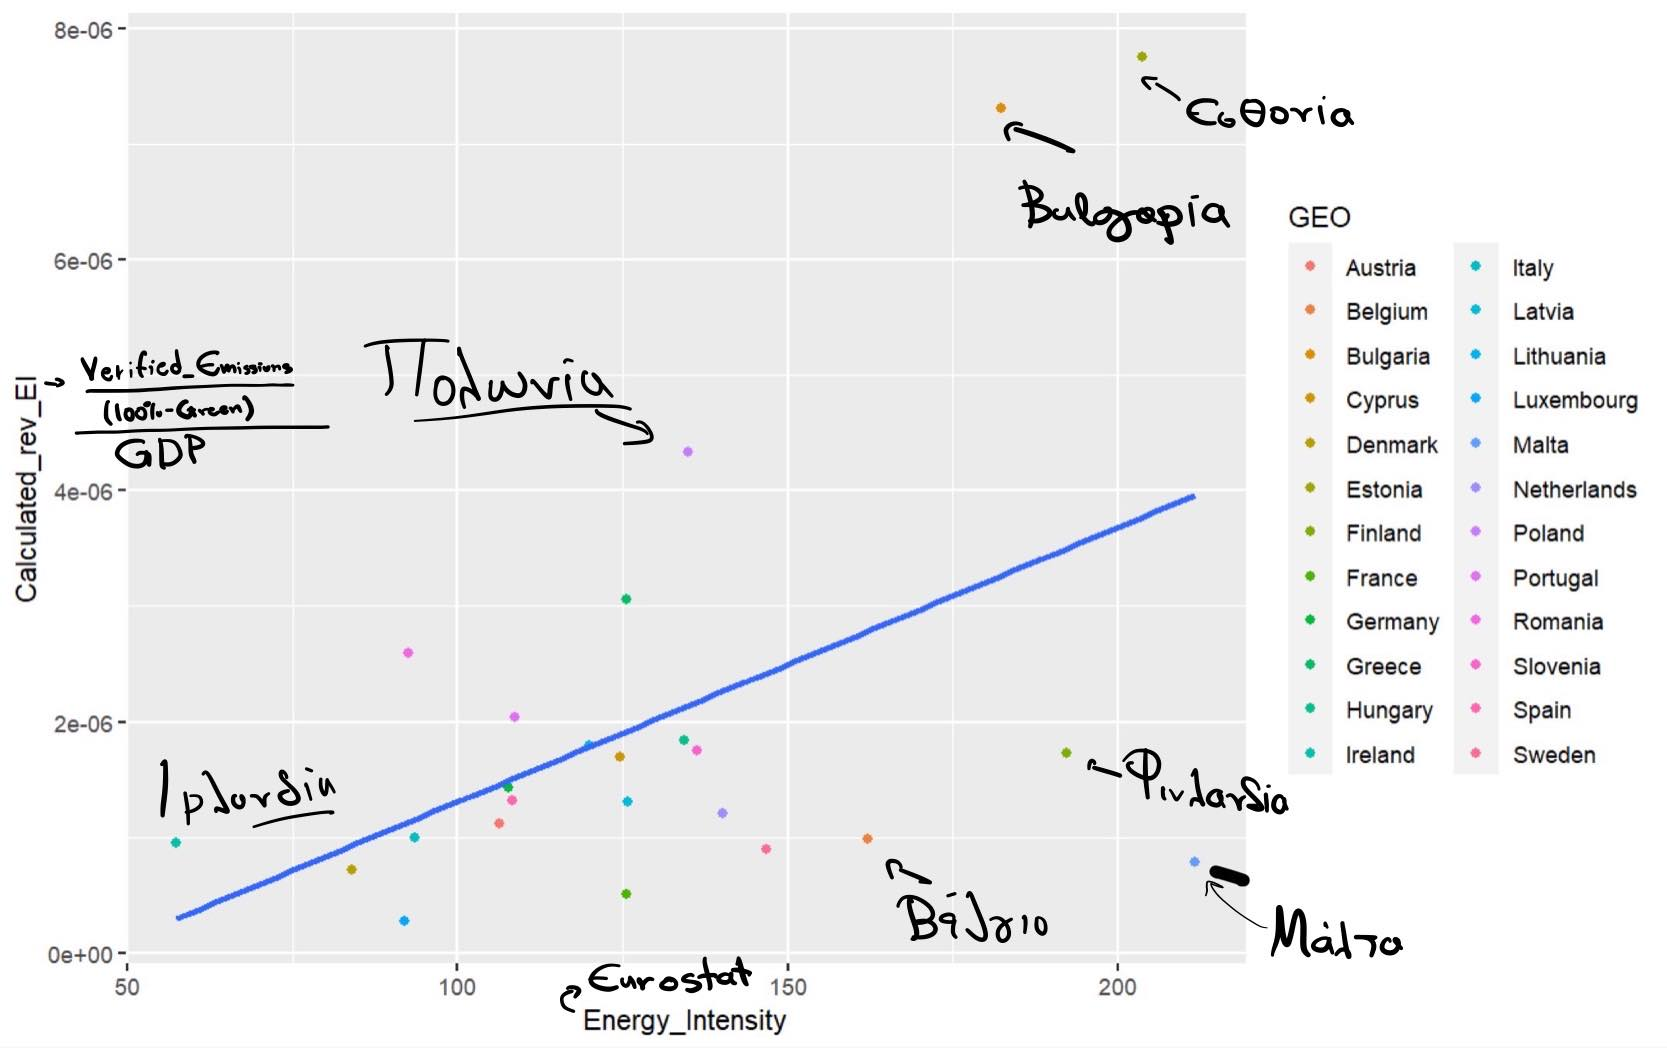
\includegraphics[width=0.7\linewidth]{images/346111264_237886352220554_6402134938597733881_n}
	\caption{Calculated Emission Intensity - Energy Intensity}
	\label{fig:3461112642378863522205546402134938597733881n}
\end{figure}


\begin{verbatim}
	Residuals:
	Min         1Q     Median         3Q        Max 
	-3.173e-06 -8.898e-07 -2.022e-07  5.596e-07  4.043e-06 
Coefficients:
Estimate Std. Error t value Pr(>|t|)  
(Intercept)          -1.065e-06  1.258e-06  -0.847   0.4061  
dat\_Energy_Intensity  2.374e-08  9.301e-09   2.553   0.0181 *
---
Signif. codes:  0 ‘***’ 0.001 ‘**’ 0.01 ‘*’ 0.05 ‘.’ 0.1 ‘ ’ 1

Residual standard error: 1.713e-06 on 22 degrees of freedom
Multiple R-squared:  0.2285,	Adjusted R-squared:  0.1934 
F-statistic: 6.516 on 1 and 22 DF,  p-value: 0.01815
\end{verbatim}
Το βασικό πρόβλημα είναι πως δεν κατάφερα να το κάνω να μοιάζει περισσότερο σε καμία εκδοχή. Ακόμα και αν βάλω στην μία πλευρά το energy supply

\begin{figure}[H]
	\centering
	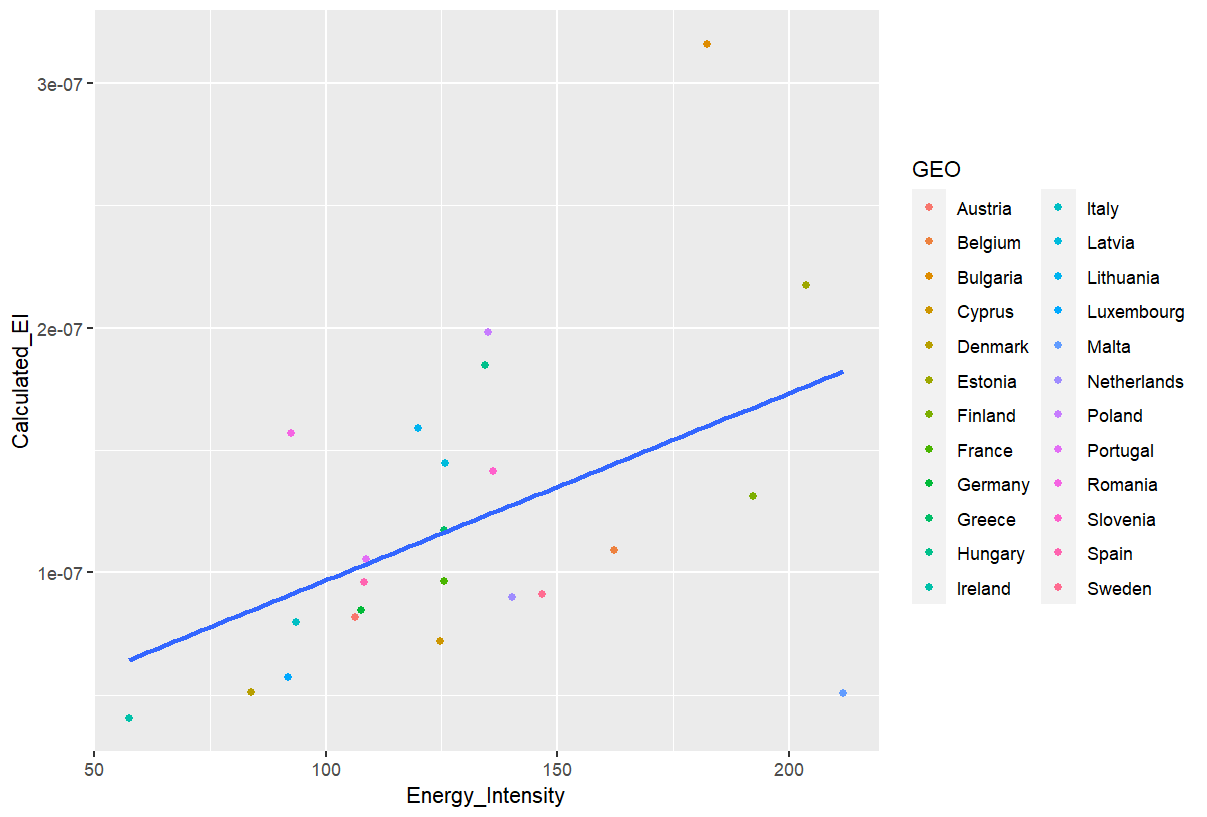
\includegraphics[width=0.7\linewidth]{images/8df6abab-b528-4c7f-a8ff-f985a8085b91}
	\caption{Calculated Energy Intensity - Energy Intensity}
	\label{fig:8df6abab-b528-4c7f-a8ff-f985a8085b91}
\end{figure}
\begin{verbatim}
Residuals:
Min         1Q     Median         3Q        Max 
-1.315e-07 -3.408e-08 -1.516e-08  3.144e-08  1.561e-07 

Coefficients:
Estimate Std. Error t value Pr(>|t|)  
(Intercept)          2.028e-08  4.200e-08   0.483   0.6339  
dat$Energy_Intensity 7.652e-10  3.106e-10   2.463   0.0221 *
---
Signif. codes:  0 ‘***’ 0.001 ‘**’ 0.01 ‘*’ 0.05 ‘.’ 0.1 ‘ ’ 1

Residual standard error: 5.722e-08 on 22 degrees of freedom
Multiple R-squared:  0.2162,	Adjusted R-squared:  0.1806 
F-statistic: 6.068 on 1 and 22 DF,  p-value: 0.02206
\end{verbatim}
\subsection{Διαφορετικά μέτρα απόδοσης / αποτελεσματικότητας}
\begin{itemize}
	\item \textbf{Energy Efficiency} Αυτό μετριέται σε Mtoe και ειλικρινά δεν μπορώ να καταλάβω από την περιγραφή του πώς διαφέρει από κάποια μορφή του total energy consumed. Έχει να κάνει με τους στόχους της EE \url{https://ec.europa.eu/eurostat/cache/metadata/en/nrg_ind_eff_esmsip2.htm} \item \textbf{Energy Productivity}  $$\frac{EconomicOutput}{RawEnergy}$$ \url{https://ec.europa.eu/eurostat/cache/metadata/en/nrg_ind_ep_esmsip2.htm}
	\item \textbf{Energy Intensity} Τα γνωστά
\end{itemize}

\subsection{Για την επόμενη φορά}
\begin{itemize}
	\item Να γίνει ο ίδιος δείκτης Energy Intensity, όμως αυτή τη φορά να μην έχει μέσα την ηλεκτροπαραγωγή, καθώς αυτή διπλομετράται. Άρα προκύπτουν δύο πειράματα:
	\begin{enumerate}
		\item Όλα τα sectors εκτός από την αεροπορία και την ηλεκτροπαραγωγή συμμετέχουν.
		\item Μόνο η ηλεκτροπαραγωγή συμμετέχει.
	\end{enumerate}
	\item Clustering σε βάθος χρόνου ώστε να δούμε αν η αλλαγές στον χρόνο επηρεάζουν το υπόλοιπο. 
	\item Clustering ανά sector 
	\item Αφαίρεσε την Μάλτα, λολ
	\item Να ξεκινήσει το LP ακόμα και με σκατά δεδομένα για να δούμε τι βγάζει!
\end{itemize}

\section{Για τις 23 Μαΐου}

\subsection{21-99 Cannot be used a proxy}
Αρχικά κατεβάζοντας από το \url{https://www.eea.europa.eu/data-and-maps/data/european-union-emissions-trading-scheme-17  # Country: All countries
} τους παραδοδέντες ρίπους, παρατηρούμε πως έχουν αυτήν την κατηγοριοποίηση:
\begin{verbatim}
[1] "20 Combustion of fuels"                                     
[2] "42 Production of bulk chemicals"                            
[3] "20-99 All stationary installations"                         
[4] "43 Production of hydrogen and synthesis gas"                
[5] "25 Production or processing of ferrous metals"              
[6] "28 Production or processing of non-ferrous metals"          
[7] "21-99 All industrial installations (excl. combustion)"      
[8] "23 Metal ore roasting or sintering"                         
[9] "36 Production of paper or cardboard"                        
[10] "33 Manufacture of mineral wool"                             
[11] "10 Aviation"                                                
[12] "26 Production of primary aluminium"                         
[13] "27 Production of secondary aluminium"                       
[14] "29 Production of cement clinker"                            
[15] "41 Production of ammonia"                                   
[16] "21  Refining of mineral oil"                                
[17] "34 Production or processing of gypsum or plasterboard"      
[18] "35 Production of pulp"                                      
[19] "38 Production of nitric acid"                               
[20] "32 Manufacture of ceramics"                                 
[21] "24  Production of pig iron or steel"                        
[22] "30 Production of lime, or calcination of dolomite/magnesite"
[23] "31 Manufacture of glass"                                    
[24] "45 Capture of greenhouse gases under Directive 2009/31/EC"  
[25] "99 Other activity opted-in under Art. 24"                   
[26] "22  Production of coke"                                     
[27] "44 Production of soda ash and sodium bicarbonate"           
[28] "37 Production of carbon black"                              
[29] "39 Production of adipic acid"                               
[30] "40 Production of glyoxal and glyoxylic acid"  
\end{verbatim}
όμως κανένα από αυτά δεν αναφέρεται στην ηλεκτροπαραγωγή συγκεκριμένα. Το πιο κοντινό ίσως είναι τα combustion fluels. Όμως κάνοντας δοκιμές για το συγκεκριμένο, καταλήξουμε πως αφαιρώντας αυτό δεν μπορούμε να καταλήξουμε σε κάποιο χρήσιμο proxy:
\begin{center}
	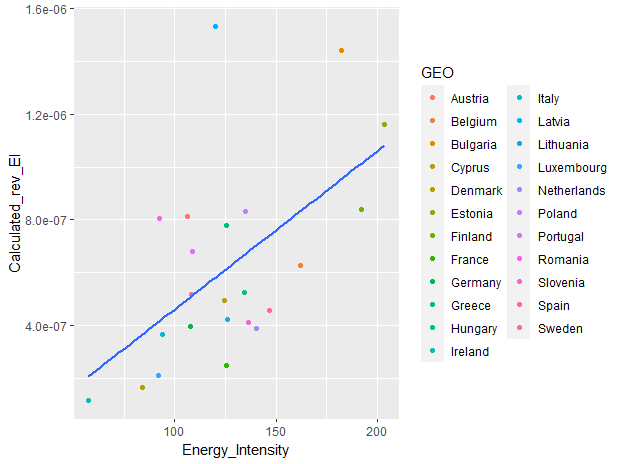
\includegraphics[width=0.7\linewidth]{images/Calculated_EI_EI_Combustion}
\end{center}

Συγκεκριμένα διαβάζουμε \cite{Guidance}: \begin{verbatim} "Most installations covered by the EU ETS will be found in the NACE categories C 
(Mining and quarrying), D (Manufacturing) and E (Electricity, gas and water supply).
 However, the activity “combustion of fuels” can occur in all types of NACE categories,
 not only industrial ones. Examples of such non-industrial installations are combustion
 units in greenhouses, hospitals, universities and office buildings, booster stations
 in natural gas transport networks etc" \end{verbatim} 
Επομένως, δεν είναι καθόλου περίεργο. Αυτό το οποίο όντως χρειάζεται να μπει σε αυτήν την διαδικασία είναι το Nace code της εταιρείας. Συγκεκριμένα έχουμε \cite{Nace1}:
\begin{verbatim}
NACE codes are the standard European nomenclature of productive economic activities.
They break down the universe of economic activities in such a way that a NACE code can
be associated with a statistical unit carrying out the activity it designates.
There is an economic activity when resources – such as capital goods – are combined
to produce specific goods or services.
All activity is characterized by the input of resources, a production process and
an output of products (goods or services).
\end{verbatim}

\subsection{Χρήση του GDPpps}
Εδώ βλέπουμε την πρώτη σημαντική βελτίωση στο αποτέλεσμα:
\begin{center}
	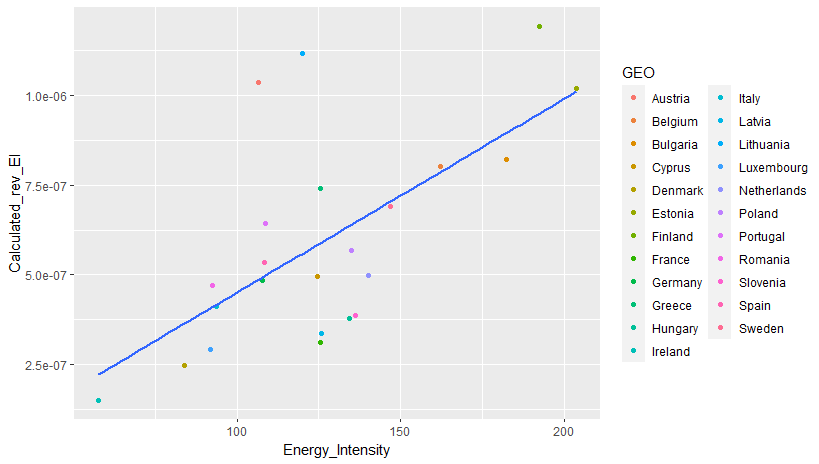
\includegraphics[width=0.7\linewidth]{images/Calculated_RI_gdpps}
\end{center}
συγκεκριμένα, η βελτίωση είναι της τάξης του:
\begin{verbatim}
	Residual standard error: 3.18e-07 on 21 degrees of freedom
	Multiple R-squared:  0.3127,	Adjusted R-squared:  0.2799 
	F-statistic: 9.553 on 1 and 21 DF,  p-value: 0.005539
	ΣΕ
	Residual standard error: 2.269e-07 on 21 degrees of freedom
	Multiple R-squared:  0.4208,	Adjusted R-squared:  0.3932 
	F-statistic: 15.26 on 1 and 21 DF,  p-value: 0.0008128
\end{verbatim}
	 Οι πιο έντονοι outliers στο παραπάνω είναι οι 3 πάνω κουκίδες που ανήκουν στην Αυστρία, Λιθουανία και την Φινλαδία από αριστερά προς τα δεξιά.

\subsection{Χωρίς Αυστρία, Λιθουανία και Φινλανδία}
Εδώ τα πράγματα βελτιώνονται, αλλά δεν είναι τέλεια:
\begin{center}
	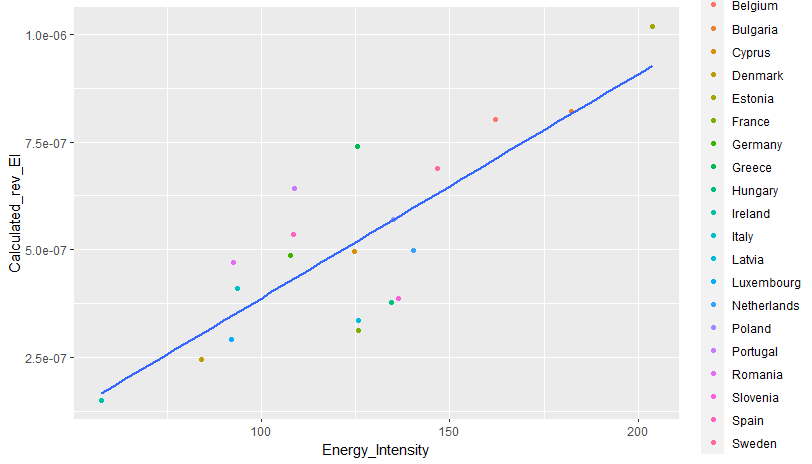
\includegraphics[width=0.7\linewidth]{images/calculated_without_austria_lithuania_finland}
\end{center}
\begin{verbatim}
	Residual standard error: 1.315e-07 on 18 degrees of freedom
	Multiple R-squared:  0.6578,	Adjusted R-squared:  0.6388 
	F-statistic:  34.6 on 1 and 18 DF,  p-value: 1.435e-05
\end{verbatim}


\newpage


\section{Για τη 13η Μαΐου}
\subsection{Το πρόβλημα με το πλασματικό energy Intensity}
Υπήρξε ένα σημαντικό κενό εδώ λόγω διαφόρων προσωπικών υποχρεώσεων. 

Αρχικά. Σχετικά με την αποδόμηση των sector των ρύπων: Έγινε αυτή η αντιστοίχιση \url{https://docs.google.com/spreadsheets/d/1mwmZSr8PBiFgsxemVE_FFEdaZS0dOeX3/edit?usp=sharing&ouid=105915891653467891041&rtpof=true&sd=truee} Το οποίο δείχνει με αρκετή σαφήνεια πως οι δύο τρόποι κατηγοριοποίησης των επιχειρήσεων είναι πολύ διαφορετικές. 

Οι πρώτες δύο στήλες αναφέρονται στα δεδομένα έτσι όπως εμφανίζονται στην βάση δεδομένων του EU ETS, ενώ οι στήλες 3,4 δείχνουν πώς αυτές εμφανίζονται στα δεδομένα της Eurostat. Προφανώς όμως κάπου υπάρχουτν αυτά τα δεδομένα, ίσως κάπου στο EU ETS, αλλά δεν ξέρω πού. Σε κάθε περίπτωση, η αντιστοίχιση θα μπορύσε να γίνει όπως φαίνεται στο παραπάνω excel. Να δύο παραδείγματα:
\\ \\
Ένα παράδειγμα στο οποίο στεκόμαστε τυχεροί:\\ \\

\begin{tabular}{|c|c|c|c|}
	\hline
	Eu ETS Code & Meaning  & Nace code &  Meaning\\
	\hline
	2 & Mineral oil refineries & C19.20 & Manufacture of refined petroleum products \\
	\hline
	21 & Refining of mineral oil & c19.10 & Manufacture of Coke and Refined Petroleum Products \\
	\hline
	22 & Production of coke & c19.10 & Manufacture of Coke and Refined Petroleum Products \\
	\hline
	3 & Coke ovens & c19.10 & Manufacture of Coke and Refined Petroleum Products \\
	\hline
	&  & C19 & Manufacture of coke and refined petroleum products \\
	\hline
\end{tabular}
Εδώ είμαστε τυχεροί γιατί μπορούμε να δουλέψουμε για το sector c19, ενώνοντας τους κωδικούς του EU ETS 2, 21, 22, 3. Αυτό θα προσφέρει λιγότερη ακρίβεια, όμως τουλάχιστον δεν θα είναι εκ προοιμίου λάθος.
\\ \\
Προβληματική περίπτωση:
\\ \\

\begin{tabular}{|c|c|c|c|}
	\hline
	Eu ETS Code & Meaning & Nace code & Meaning \\
	\hline
	&  & C23 & Manufacture of other non-metallic mineral products \\
	\hline
	29 & \makecell{Production of\\cement clinker} & C23.5.1  & Manufacture of cement \\
	\hline
	30 & \makecell{Production of\\ lime, or calcination\\ of dolomite/mag...} & C23.5.2 & Manufacture of lime and plaste \\
	\hline
	31 & Manufacture of glass & C23.1 & Manufacture of glass and glass products \\
	\hline
	32 & Manufacture of ceramics & C23.4 & Manufacture of other porcelain and ceramic products \\
	\hline
	33 & Manufacture of mineral wool & C23.9.9 & \makecell{Manufacture of other non-metallic\\ mineral products n.e.c.} \\
	\hline
	34 & \makecell{Production or processing\\ of gypsum or plasterboard} & C23.5.2 & Manufacture of lime and plaster \\
	\hline
	&  & C23.2 & Manufacture of refractory products \\
	\hline
	&  & C23.3 & Manufacture of clay building materials \\
	\hline
	&  & C23.6 &\makecell{ Manufacture of articles of concrete,\\ cement and plaster} \\
	\hline
	&  & C23.7 & Cutting, shaping and finishing of stone \\
	\hline
	&  & C23.9.1 & Production of abrasive products \\
	\hline
\end{tabular} \\  \\
Εδώ έχουμε ένα σενάριο στο οποίο όχι μόνο δεν ταιριάζουν όλα απόλυτα, αλλά ακόμα και να την αριστερή στήλη σε ένα για να την ταυτίσουμε με την δεξιά, θα υπάρχουν κατηγορίες τις οποίες αφήσαμε απ' έξω.

\subsection{Clustering se sectors}
Querry για να πάρουμε τις Surrendered άδειες ανά sector για το 2016. 
\begin{verbatim}
	SELECT SUM(trnew.NbOfUnits), concat(mat.kwdikos , ' ' , mat.onoma) as ActivityType
	FROM transactions_new AS trnew
	JOIN eutl_accountholders AS ah ON trnew.TransferringAccountHolder = ah.holderName
	JOIN eutl_accounts AS a ON ah.rawCode = a.rawCode
	JOIN eutl_installations_orair AS io ON io.account = a.rawCode
	JOIN mainactivitytype AS mat ON io.mainActivity = mat.kwdikos
	WHERE trnew.TransactionType LIKE '%%-2' AND YEAR(trnew.TransactionDate) = 2016
	GROUP BY mat.onoma
	ORDER BY mat.kwdikos
\end{verbatim}
To οποίο επιστρέφει: \\ \\
\begin{tabular}{|c|c|}
	\hline
	Surrendered & ActivityType \\
	\hline
	178093310 & 1 Combustion installations with a rated thermal in... \\
	\hline
	287282477 & 10 Aircraft operator activities \\
	\hline
	4028607 & 2 Mineral oil refineries \\
	\hline
	697984775 & 20 Combustion of fuels \\
	\hline
	6795214 & 21 Refining of mineral oil \\
	\hline
	187557 & 22 Production of coke \\
	\hline
	179735 & 23 Metal ore roasting or sintering \\
	\hline
	98482418 & 24 Production of pig iron or steel \\
	\hline
	21458739 & 25 Production or processing of ferrous metals \\
	\hline
	806566 & 26 Production of primary aluminium \\
	\hline
	2287866 & 27 Production of secondary aluminium \\
	\hline
	16525496 & 28 Production or processing of non-ferrous metals \\
	\hline
	9283720 & 29 Production of cement clinker \\
	\hline
	29011461 & 30 Production of lime, or calcination of dolomite/... \\
	\hline
	28483791 & 31 Manufacture of glass \\
	\hline
	113925371 & 32 Manufacture of ceramics \\
	\hline
	855132 & 33 Manufacture of mineral wool \\
	\hline
	2350152 & 34 Production or processing of gypsum or plasterbo... \\
	\hline
	34482572 & 35 Production of pulp \\
	\hline
	120320357 & 36 Production of paper or cardboard \\
	\hline
	3530168 & 37 Production of carbon black \\
	\hline
	10773361 & 38 Production of nitric acid \\
	\hline
	3665 & 39 Production of adipic acid \\
	\hline
	205592 & 40 Production of glyoxal and glyoxylic acid \\
	\hline
	518707 & 41 Production of ammonia \\
	\hline
	51838556 & 42 Production of bulk chemicals \\
	\hline
	8355618 & 43 Production of hydrogen and synthesis gas \\
	\hline
	4930431 & 44 Production of soda ash and sodium bicarbonate \\
	\hline
	10617 & 46 Transport of greenhouse gases under Directive 2... \\
	\hline
	1853546 & 5 Installations for the production o...ion) includ... \\
	\hline
	12267703 & 6 Installations for the production o...rotary kiln... \\
	\hline
	1787688 & 7 Installations for the manufacture of glass inclu... \\
	\hline
	18284476 & 8 Installations for the manufacture ...ks, tiles, ... \\
	\hline
	21850482 & 9 Industrial plants for the producti...ous materia... \\
	\hline
	42185334 & 99 Other activity opted-in pursuant to Article 24 ... \\
	\hline
\end{tabular}

\subsection{Τι ειπώθηκε στην κλίση}
Στην κλίση τέθηκαν οι παρακάτω στόχοι:
\begin{itemize}
	\item Να γίνει το LP χρησιμοποιώντας τους 5 sectors έτσι όπως έγιναν λόγω των περιορισμών των δεδομένων. Άρα όπως είναι στο excel τα διαφορετικά χρώματα:  \url{https://docs.google.com/spreadsheets/d/1mwmZSr8PBiFgsxemVE_FFEdaZS0dOeX3/edit?usp=sharing&ouid=105915891653467891041&rtpof=true&sd=truee}
	\item Να γίνει clustering  στους διαφορετικούς sectors. Χρησιμοποίησε Querries σαν αυτό που ανέφερες λίγο παραπάνω για να αποκτήσεις δεδομένα για τους διαφορετικούς κλάδους της οικονομίας. Παραδείγματα: Verified, Free, no of companies, avg transactions per company, μέγεθος εταιρειών 
	\item Να προσπαθήσεις να δεις γιατί κάποιες χώρες δεν αντιστοιχίζονται τέλεια στα διαγράμματα τα οποία υποβάλαμε στο paper. Μερικές πιθανές συσχετίσεις: ποσοστό service στο ακαθάριστο προϊόν, πυκνότητα σε εταιρείες με πολύ μεγάλο ή πολύ μικρό P(carbon leackage). 
	\item Να ξαναγίνει η μελέτη που γίνεται στο paper μόνο για έναν από τους sectors της οικονομίας και να δούμε αν αυτό μιδενίζει τις διαφορές μεταξύ των χωρών. 
	\item Διάβασμα τo paper: Pollution Permits: Efficiency by Design \url{https://papers.ssrn.com/sol3/papers.cfm?abstract_id=4453956}
\end{itemize}

\section{Παύση Καλοκαιριού}
Ρεαλιστικά δεν έγιναν όσα πράγματα θα έπρεπε από μέρους μου. Προοέκυψαν πολλές δουλειές άσχετες με την σχολή πάνω στην εξεταστική, με αποτέλεσμα αυτή να πάει πολύ άσχημα. Τα βασικά αίτια ήταν το ότι αναλαμβάνω πράγματα που δεν πρέπει και πάντα έχω μπροστά μου ένα βουνά που η αναβλητικότητά μου δεν με αφήνει να νικήσω. Θα το αλλάξω. 

\section{Επανεκκίνηση Μετά την παύση του καλοκαιριού}



\subsection{Polution Permits: Efficiency by Design}
Οι γνώσεις μου είναι υπερβολικά λίγες για να καταλάβω το περιεχόμενο αυτού του paper.

\subsection{Παρουσίαση για το paper}

	
  
\subsection{1 sector}
Ακριβώς ένα sector ίσως να γίνεται μόνο όσων αφορά στα δεδομένα της βάσης του ETS, οπότε δεν θα χρησιμοποιήσουμε άλλα 
	
\section{Συνάντηση στο ΜΟΠ 10/10/23}
Στη συνάντηση που πραγματοποιήθηκε στις 10 Οκτωβρίου 2023 στο ΜΟΠ, συζητήθηκαν σημαντικά ζητήματα σχετικά με την ερευνητική προσέγγιση και τους πιθανούς στόχους της διπλωματικής.

\subsection{Προκύπτοντα ερωτήματα}
Κατά τη διάρκεια της συζήτησης προέκυψαν τα εξής ερωτήματα:

\begin{enumerate}
	\item Είναι δύσκολο να εφαρμόσουμε τεχνικές clustering ανά εταιρεία λόγω της έλλειψης δεδομένων. Υπάρχει όμως η πιθανότητα για μεγάλες εταιρείες να έχουν δημοσιευμένα δεδομένα που μπορεί να χρησιμοποιηθούν;
\end{enumerate}

\subsection{Προτεινόμενοι στόχοι}
Στη συνέχεια της συνάντησης, προτάθηκαν κάποιοι στόχοι για την ερευνητική διαδικασία:

\begin{enumerate}
	\item Διαχωρισμός των προσεγγίσεων: Αρχικά, να καθοριστεί αν μπορούμε να παράγουμε απλώς συμπεράσματα ή αν μπορούμε να προτείνουμε συγκεκριμένες τεχνικές. Είναι σαφές ότι ο στόχος πρέπει να είναι η προσφορά συγκεκριμένων τεχνικών.
	\item Επανάληψη των βημάτων του paper: Ακολουθώντας τις ίδιες διαδικασίες όπως στο paper, να εξετάσουμε αν η τεχνική Linear Programming (LP) μπορεί να λύσει τα διάφορα προβλήματα, ειδικά όταν ομαδοποιούμε τις εταιρείες.
	\item Σύγκριση τεχνικών: Να δούμε αν η τεχνική "Allocating Emission Permits" παράγει αποτελέσματα που είναι κοντά στα αποτελέσματα του LP.
	\item Ορισμός concept για τη διπλωματική: Είναι ζωτικής σημασίας να καθορίσουμε ένα σαφές concept για την διπλωματική, το οποίο θα κατευθύνει όλες τις ερευνητικές προσπάθειες.
\end{enumerate}

\section{Συνάντηση στο ΜΟΠ 31/10/23}
Στη συνάντηση που πραγματοποιήθηκε στις 31 Οκτωβρίου 2023 στο ΜΟΠ, συζητήθηκαν οι εξής σημαντικές πτυχές:

\subsection{Σημαντικά Ειπωθέντα}
\begin{itemize}
	\item Η Τζέλα ανέβασε στο drive ένα άρθρο που περιέχει τη διάσταση του χρόνου, με κλειδί λέξεις όπως uncertainty και αναφορά στην παράγραφο 3.
	\item Το abatement μπορεί να αναλυθεί σε δύο κατευθύνσεις: ρίποι και προϊόν.
\end{itemize}

\subsection{Στόχοι}
\begin{enumerate}
	\item Δοκίμασε το τελευταίο paper για να δεις αν λειτουργεί εντός του LP και αν περιλαμβάνει κάποια μορφή fairness όπως έχει οριστεί.
	\item Προσπάθησε να κατανοήσεις πλήρως το μοντέλο του paper και συγκρίνε το με το LP.
	\item Ολοκληρώστε τον καθαρισμό του κώδικα.
	\item Δημιουργήστε ένα συνθετικό dataset. Θα χρειαστείς κανόνες για την επόμενη συνάντηση για να κάνεις το dataset να λειτουργεί, όπως κριτήρια συνοχής για τα συνθετικά sectors, GDP κ.λπ. Επίσης, η ισορροπία Cournot θα βοηθήσει στον καθορισμό της τιμής του προϊόντος ανά sector.
\end{enumerate}

\section{Συνάντηση μέσω Skype στις 5 Νοεμβρίου 2023}
Η συζήτηση πραγματοποιήθηκε μέσω Skype στις 5 Νοεμβρίου 2023 και επικεντρώθηκε στη δημιουργία συνθετικών δεδομένων για τη διπλωματική.

\subsection{Δημιουργία Συνθετικών Δεδομένων}
Στόχος είναι η παραγωγή συνθετικών δεδομένων για τρεις χώρες και τρεις τομείς σε κάθε χώρα, με την εκπροσώπηση τεσσάρων εταιρειών ανά τομέα. Τα δεδομένα θα καλύπτουν τις παρακάτω πτυχές:

\begin{enumerate}
	\item Energy Intensity
	\item Ακαθάριστο Εγχώριο Προϊόν ανά τομέα
	\item Εκπομπές ρύπων ανά τομέα
\end{enumerate}

Επιπρόσθετα, η κλίμακα κάθε εταιρείας θα πρέπει να σχετίζεται με το μέγεθος της αντίστοιχης χώρας.

\subsection{Ανάλυση Εταιρικών Συναρτήσεων}
Η συζήτηση αφορούσε επίσης τις εταιρικές συναρτήσεις και τους κανόνες που τις καθορίζουν. Σημαντικά σημεία περιλαμβάνουν:

\begin{enumerate}
	\item Η ανάγκη μελέτης του τρίτου κεφαλαίου του ΑΟΘ. Από εμένα, γιατί είμαι άσχετος.
	\item Η συνάρτηση "abatement" θεωρείται ως φθίνουσα, με μηδενική τιμή στις εκπομπές Business as Usual και άπειρη τιμή στις μηδενικές εκπομπές.
	\item Το κόστος παραγωγής αποτελείται από το άθροισμα σταθερών και μεταβλητών κοστών, με χαρακτηριστική φθίνουσα απόδοση.
	\item Το τελικό κόστος ανά προϊόν αποτελεί αυξανόμενη κυρτή συνάρτηση.
\end{enumerate}

\subsection{Στόχοι για την Επόμενη Συνάντηση}
Ως επόμενο βήμα, προτείνεται η εκπόνηση πέντε λογικών συναρτήσεων που θα εφαρμόζονται στα προαναφερθέντα δεδομένα.

\section{Συνάντηση στο ΜΟΠ στις 7 Νοεμβρίου 2023}

\subsection{Πριν την συνάντηση}
\subsubsection{Ορισμοί}
\begin{itemize}
	\item Η παραγωγή $q_i$ θα είναι η ελέυθερη μεταβλητή στο πρόγραμμά μας.
	\item Στο paper ορίζει το abatement ως non-decreasing και convex, σε αντίθεση με τον ορισμό του Σωτήρη, ο οποίος ορίζει πάλι κυρτή συνάρτηση αλλά φθήνουσα. Η διαφορά είναι πως η μία παίρνει για είσοδο την μείωση των ρίπων, ενώ η δεύτερη παίρνει για είσοδο τους τελικούς ρύπους. 
	\item Η συνάρτηση απόδοσης των δωρεάν αδειών είναι κοίλη.
	\item $x_i^*$ ορίζονται οι ρύποι ύστερα από τον συνυπολογισμό των δωρεάν αδειών για την εταιρεία i . $q_i^*$ ομοίως είναι η παραγωγή μετά από τον υπολογισμό. Ορίζεται επίσης η διαφορά $q_i^* - x_i^*$ ως το μέγεθος του abatement. 
\end{itemize}

\subsubsection{Πιθανές συναρτήσεις παραγωγής}
Η συνάρτηση για το κόστος παραγωγής μπορεί να έχει τις παρακάτω μορφές:
\begin{enumerate}
\item Γραμμική : FC + Bx, οπου Α τα σταθερά κόστη και B το οριακό κόστος ανά μονάδα.
\item Κυρτή αύξουσα : $FC+ Ae^{\lambda x}$
\item Αλλγη κυρτή αύξουσα: $FC + Αx^\lambda$
\item Συνυπολογίζουσας τις οικονομίες κλίμακας (chat gpt): $TC(n) = FX + \frac{VC}{1+an} \times n$. 
\item Πάλι από το GPT: $TC(n) = FC + nVC + SC(n)$ , οπου το SC είναι το Scaling cost.
\end{enumerate}
\subsubsection{Abatement cost}
Το abatement cost μπορεί να αναχθεί από τον ορισμό του Σωτήρη στον ορισμό που καταλαβαίνει το κεφάλι μου απλά με την αλλαγή $Sot(Actual, BAU) = C(BAU-Actual)$. Αν θέλουμε να παίρνει για είσοδο ποσοστό τότε η αντιστοιχία είναι: 
$$ Sot(Actual, BAU) = C(\frac{BAU-Actual}{BAU}\times 100\%)$$
Πιθανές συναρτήσεις για abatement είναι:
\begin{enumerate}
\item   $g(x) = Ae^{\lambda x}$
\item  $g(x) = ax^2 + bx+ c$
\item  GPT: $c(e^{bx}-1), ax^3 ...$
\item  GPT: $ln(x)$ το οποίο δεν βγάζει κανένα νόημα. 
\end{enumerate}

Συναρτήσεις που ταιριάζουν με τον ορισμό του Σωτήρη είναι:
\begin{enumerate}
\item $\frac{1}{x} - \frac{1}{BAU}$
\item $\frac{1}{x^2}$
\end{enumerate}

\subsection{Τι είπαμε στην συνάντηση - Ορισμός προβλήματος}

Αρχικά βρήκα τον κύβο μου! (τον 11 M pro, ο i3 ακόμα αγνοείται) (ναι, δεν είναι τόσο σημαντικό αυτό, αλλά και είναι λίγο)

\begin{itemize}
	\item Ν εταιρείες.
	\item C χώρες.
	\item S τομείς της αγοράς. 
	\item $\tau$ κόστος της άδειας.
	\item $E_s: q_i \rightarrow x_i $ ρυθμός ρύπων για τον τομέα s
	\item $q_{i,y}$ παραγωγή της εταιρείας με id = i και έτος = y.
	\item $q_i$ παραγωγή της εταιρείας με id = i, για ανάλυση μίας χρονιάς.
	\item $q_i^* = q_{i,y+1}$
	\item $χ_{i,y}$ ρύποι της εταιρείας με id = i και έτος = y.
	\item $χ_i$ ρύποι της εταιρείας με id = i, για ανάλυση μίας χρονιάς.
	\item $χ_i^* = χ_{i,y+1}$
	\item $\Phi_i(y)$ = δωρεάν άδειες για το έτος y στην εταιρεία i.
	\item C(i) = επιστρέφει την χώρα της εταιρείας i.
	\item S(i) = επιστρέφει τον τομέα της εταιρείας i.
	\item $K_{c,s,y} = \sum{x_{i,y}}, \forall x_{i,y} | y=y \wedge c = C{i} \wedge S(i) = s$
	\item $Q_{c,s,y} = \sum{q_{i,y}}, \forall x_{i,y} | y=y \wedge c = C{i} \wedge S(i) = s$
	\item $p_s(y)$ η αντίστροφη συνάρτηση ζήτησης για το προϊόν του τομέα s για το έτος y. Κοίλη και φθίνουσα. $ p_s : Q \rightarrow \R$, όπου $\R$ εδώ είναι η τιμή πώλησης.
	\item $f_i(y)$ η συνάρτηση abatement, κυρτή, αύξουσα με $f(0)=0 \wedge f'(0) = 0 \wedge f_i(x) \forall x \geq 0$
	\item $pr_i(q_{i,y})$ κόστος παραγωγής για την εταιρεία. Όπως είπαμε είναι ξεχωριστή συνάρτηση για την κάθε εταιρεία, κυρτή και αύξουσα. Σε αντίθεση με το paper \cite{Allocating} όπου το οριακό κόστος είναι σταθερό.
\end{itemize}

Κέρδος επιχείρησης:
$$ p_s (\sum {q_j^*} \forall j | S(j) = S(i))- \tau (x_i^* - \Phi_i)- pr_i(q_i*) - f_i(E_s(q_i)- x_i^*)	  $$
\subsubsection{Βήμα 1}
Στη συνέχεια θέσαμε με πολλή σαφήνεια τους στόχους.Επομένως προκύπτει ο παρακάτω ορισμός προβλήματος:

\begin{itemize}
	\item Θα φτιάξουμε 1 εταιρεία για κάθε j από τους 3 τομείς για κάθε μία χώρα i από τις 3 στα συνθετικά δεδομένα. 
	\item  Καλό είναι στα δεδομένα αυτά να έχουμε έναν μπουσουλα στην αρχή, οπότε οι 3 χώρες θα μοιάζουν με την Ιταλία, τη Γερμανία και την Ολλανδία. 
	\item Αντίστοιχα, οι τομείς θα μοιάζουν με τους τομείς: τσιμέντα, ηλεκτροπαραγωγή, παραγωγή χαρτιού.
	\item Για κάθε τομέα θα χρησιμοποιήσουμε μία συνάρτηση ρυθμού ρύπων, άρα 3 συναρτήσεις.
	\item Θα χρειαστούμε επίσης 1  συνάρτηση ζήτησης για κάθε τομέα, άρα 3 συναρτήσεις φθίνουσες.
	\item Οι συναρτήσεις abatement θα είναι ξεχωριστές για όλους, άρα 9.
	\item Ομοίως, και οι 9 συναρτήσεις production. 
	\item Η τιμή της άδειας θα θεωρείται σταθερή.
	\item Το κόστος παραγωγής θα είναι γραμμική αύξουσα.
	\item Το abatement θα ορίζεται ως μπλα μπλα.
\end{itemize}

\subsubsection{Βήμα 2}

Αφού οριστούν αυτά θα πρέπει να βρεθεί ο Cournot ισορροπία. Στο σύστημα.

Μετά τα δεδομένα αυτά θα feedαριστούν στο LP, τον Linear Mechanism του άρθρου \cite{Allocating} και ιδανικά και στο benchmarking. 

\subsubsection{Βήμα 3 - Βελτιώσεις}
Χωρίς κάποια συγκεκριμένη σειρά πρέπει να γίνουν τα παρακάτω:
\begin{itemize}
	\item Η τιμή της άδειας να ορίζεται από το Cap and Trade σύστημα.
	\item H συνάρτηση κόστους παραγωγής να γίνει κυρτή. Πιθανώς πολυώνυμο τρίτου βαθμού καθώς το marginal cost του παναγιώτη ήταν δευτέρου.
	\item Η συνάρτηση του abatement να γίνει απειρίζουσα κυρτή.
	\item Να μπουν παραπάνω εταιρείες ανά sector.
	\item Παραπάνω χώρες. 
	\item Παρακάτω τομείς. 
\end{itemize}

\section{Συνάντηση 14 Νοεμβρίου 2023 στο ΜΟΠ}
\begin{enumerate}
	\item Είπαμε πως στην αρχή το κόστος παραγωγής θα είναι 0. h=0, άρα δεν χρειάζεται να γίνει κάτι διαφορετικό από αυτό που κάνουν στο paper \cite{Allocating}.
	\item Βασάνισες πολύ την Τζέλα, χρωστάς καφέ / ποτό.
	\item Πρέπει να διαβάσω το \cite{Allocating} για να καταλάβω καλύτερα το μηχανισμό του regulator. 
\end{enumerate}  

Μερικές απορίες που έχω και οι οποίες δεν λύνονται νομίζω κάπως:
\begin{enumerate}
	\item Στην ερώτηση είχα σημειώσει ένα συγκεκριμένο παράδειγμα, αλλά αυτό το ερώτημα θα μπορούσε να γραφτεί και ως: Πώς διαχειριζόμαστε τις διαφορές στην πληροφορία μεταξύ των εταιρειών;
	\item Πώς μπορούμε να βάλουμε στο σύστημα επιπλέον στοιχεία ρτεαλισμού, όπως την ανελαστικότητα της παραγωγής για κάποια προϊόντα ή το ότι αν μία επιχείριση σταματήσει φέτος την παραγωγή της, ίσως να μην είναι εφικτό να την επαναφέρει την επόμενη χρονιά, οπότε ίσως να πρέπει να το συνυπολογίσει αυτό.

\end{enumerate} 

\section{Συνάντηση 28 Νοεμβρίου 2023}
Ακύρωσα την προηγούμενη Τρίτη. 
Διάβασα για το cournot competition.
Αλλά και εκείνη την φορά πήγα από ντροπή. Δεν είχα κάτι καινούριο να πω ή δεν είχα κάνει κάτι παραπάνω.
Μετά ακύρωσα και την επόμενη εβδομάδα, επειδή ήταν το Πρώτο Εθνικό πρωτάθλημα ταχυκυβισμού. 


\section{Συνάντηση στις 12/12/23}
Ξεκίνησα να γράφω τον κώδικά για όσα είπαμε. Ήταν καλύτερος από όλα τα προηγούμενα, αλλά ακόμα ήταν χάλια. Απέτυχα να έρθω στην συνάντηση.


\section{Συνάντηση στις 19/12/23}
Ξαναέπιασα τον κώδικα από την αρχή. Πλέον εμφανώς πλίγομαι σε μία κουταλιά νερό. Αλλά προσπαθώ και πάει καλά νομίζω.

\section{Διαδικτυακή συνάντηση 27/2/24}
Καταλήψεις, ιστορίες κλπ. Δεν είχα διαβάσει αρκετά παρόλο που αυτό το διάστημα αυτό υποτίθεται πως έκανα. 

Μία μικρή περίληψη των παλιών είναι: 
\begin{enumerate}
	\item Χρησιμοποιώντας 3 sectors και ομογενή προϊόντα και 3 χώρες και 3 εταιρείες ανά sector να λυθεί το πρόβλημα του cournot competition όπως αυτό ορίζεται από το \cite{Allocating}.
	\item Στην συνέχεια, να δούμε πόσο κοντά μπορεί να φτάσει το γραμμικό πρόγραμμα που ορίσαμε στο άρθρο \cite{First}. 
	\item Αφού δούμε τα αποτελέσματα σε αυτό, πρέπει να δούμε πού και γιατί αποτυγχάνει. Μπορεί να εξηγηθεί κάπως;
	\item Ίδια δουλειά, αλλά με τον αλγόριθμο του benchmarking. 
	\item Διεύευνση για πολλά data.
	\item Μεταφορά στα πραγματικά data. 
\end{enumerate}
Επιπλέον χρήσιμα πράγματα που ειπώθηκαν ήταν:
\begin{enumerate}
	\item Πολύ ενδιαφέρον paper το \cite{'2269'}, το οποίο αξίζει να το διαβάσω για να καταλάβω το social welfare. 
	\item Δες τον πίνακα 3 από την διπλωματική του Παναγιώτη.
\end{enumerate}
Παράλληλα, στα νέα των παιδιών είναι: Ο Σωτήρης μετακόμισε και μείωθηκαν οι υπερωρίες. Στην δουλειά είχε γίνει κάποιο λάθος στο πρότζεκτ της δουλειάς, γιατί λείπανε τιμές από τελικές εξετάσεις, για μία εξέταση που δεν καταγράφεται, αλλά επαναλαμβάνεται κάθε μισή ώρα. Επίσης, είχε πάει Φλοίσβο το Σάββατο και κρύωσε. Κάποια στιγμή επίσης πρέπει να χειρουργήθηκε η γιαγιά του στο Ωνάδιο για αλλαγή μητροειδούς. 
Η Τζέλα ακόμα τελειώνει το διδακτορικό, όμως έχει πέσει η αποδοτικότητά της, όχι η όρεξή της για όλο αυτό. Μετά έρχεται το μεταδιδακτορικό. 

	\section{Επανεκκίνηση 22/4/24}
Πλάνο για το επόμενο διάστημα:
\begin{enumerate}
	\item Οργάνωσε όντως τον παλιό κώδικά. Όχι εσύ, βάλε το τσατ να το κάνει. Αλλά να γίνει καλά και γρήγορα. 
	\item Ξαναδιάβασε σωστά το \cite{Allocating}.
	\item Βάλε επιπλέον ένα μοντέλο το οποίο θα έχει όλες τις πληροφορίες πάνω του και θα μπορείς να του τρέξεις διαφοετικά πράγματα. 
	\item Χρησιμοποιώντας 3 sectors και ομογενή προϊόντα και 3 χώρες και 3 εταιρείες ανά sector να λυθεί το πρόβλημα του cournot competition όπως αυτό ορίζεται από το \cite{Allocating}.
	\item Στην συνέχεια, να δούμε πόσο κοντά μπορεί να φτάσει το γραμμικό πρόγραμμα που ορίσαμε στο άρθρο \cite{First}. 
	\item Αφού δούμε τα αποτελέσματα σε αυτό, πρέπει να δούμε πού και γιατί αποτυγχάνει. Μπορεί να εξηγηθεί κάπως;
	\item Ίδια δουλειά, αλλά με τον αλγόριθμο του benchmarking. 
	\item Διεύευνση για πολλά data.
	\item Μεταφορά στα πραγματικά data. 
\end{enumerate}

\section{Επανεκκίνηση 19/7/24}
Ξεκίνημα ξανά. Πάμε. Οι γενικοί στόχοι μένουν ίδιοι. Γενικά έγιναν τα παρακάτω:
\begin{enumerate}
	\item Απέτυχα να χρησιμοποιήσω κάποιο από τα Pyomo ή XCvCV για να τρέξω ακόμα και ένα απλό προβλημα στη python.
	\item Δοκιμάζω το Gurobi που μου είχε πει η Αθηνά. 
	\item Τελικά μια χαρά λειτουργεί το Gurobi. Επίσης, μία χαρά λειτουργεί η δημιουργία των dummy data. 
	\item Κάθε αντικείμενο θα έχει την δική του συνάρτηση, άρα μπορούμε να μοντελοποιήσουμε κανονικά όσες τιμές θέλουμε. Δεν ξέρω γιατί 3 μέρες δουλειάς μπορούν να αντικατασταθούν από 40 λεπτά με chat Gpt...
\end{enumerate}
Προφανώς έγιναν και άλλα πράγματα όσο ήμουν στην Σαντορίνη, αλλά δεν τα κατέγραψα. Τα πιο σημαντικά ήταν το να διαβάσω ξανά τα 2 σημαντικά paper. Το submission 2269 η αλήθεια είναι πως δεν το κατάλαβα, το καλύτερο δε είναι η κοστολόγηση της εκτύπωσης στην όμορφη Σαντορίνη, αλλά τι να κάνουμε...

\section{Συνάντηση με τον κ Φωτάκη από το γραφείο του Κοινοτάρχη Αστριτσίου 26 Ιουλίου}

Στην συνάντηση ειπώθηκαν αρκετά πράγματα. Στην αρχή ήταν και η Τζέλα εκεί και για τα νέα να πούμε πως ΠΑΡΟΥΣΙΑΖΩ ΤΕΛΗ Οκτωβρίου! Επίσης, η Τζέλα πήγε και παρουσίασε στις Βρυξέλλες το paper που είχαν γράψει με τον Παναγιώτη, καθώς πήρε βραβείο καλύτερου paper. Επίσης, ειπώθηκε η τρομερή ατάκα "Δεν μπορείς να μείνεις παραπάνω στην σχολή, κάνεις κακό στον εαυτό σου".

Στην συνέχεια αποχώρησε η Τζέλα και το θέμα της συζήτησης ήταν το μέλλον μου και προοπτικές σχετικές με την διδασκαλία. Σε αυτό προφανώς υπάρχουν δύο πολύ διακριτοί δρόμοι. Από εδώ και πέρα θα παραφράζω και θα γράψω σε πρώτο πρόσωπο σαν να μιλάει ο κ Φωτάκης, αλλά προφανώς δεν τα θυμάμαι αρκετά καλά. 


Μην πας στο σχολείο. Θα το μετανιώσεις επειδή: 1) Είναι σε κακό επίπεδο η εκπαίδευση στην Ελλάδα 2) Είναι σε ακόμα χειρότερο επίπεδο η εκπαίδευση στην πληροφορική 3) Είναι πολύ εύκολο να βρεθείς να εξαρτάσαι από διευθυντές που θα σου κάνουν δύσκολη τη ζωή χωρίς κάποιο λόγο 4) Τα τυπικά σου προσόντα θα δημιουργούσαν μεγαλύτερες προσδοκίες 5) Δεν θα σου επιστρέψει όσα θα του δώσεις εσύ.

Η άλλη εκδοχή είναι να γίνεις ΕΔΙΠ. Όμως αυτό είναι μία πολύ μεγαλύτερη δέσμευση και δυσκολότερο. Αυτό που κερδίζεις είναι πως θα νιώθεις να πιάνει τόπο η δουλειά σου και να νιώθεις περήφανος. Αλλά για αυτό χρειάζεσαι διδακτορικό και εννοείται να συμμετέχεις στην έρευνα. Γιατί η έρευνα είναι η επικαιροποίηση της γνώσης σου. 

Παράλληλα όσο μιλούσαμε τον πήρε τηλέφωνο ένας φίλος του, ο οποίος είχε αδικηθεί πολύ στην δουλειά του. Παντού θα παίζουν αυτά, αλλά ήταν πολύ άσχημο και η ζωή ενός ανθρώπου πήγε πίσω αρκετά χρόνια, απλά επειδή κάποιος άλλος είχε τις γνωριμίες μάλλον...

Γυρνώντας πίσω στα εκπαιδευτικά. Προφανώς είναι χαμηλότερος ο μισθός στην εκπαίδευση και αυτό πρέπει να είναι κάτι που το γνωρίζεις από πριν. 

Το μεταπτυχιακό Εδέμ θα σου ταίριαζε. Ουσιαστικά ταιριάζει στην διπλωματική σου, σου προσφέρει παραπάνω γνώσεις πάνω στο αντικείμενο, είναι τίγκα στα buzz words και ανεβάζει την αγοραστική σου αξία. Ρεαλιστικά ξεκινώντας το ΕΔΕΜ θα συμβούν δύο πράγματα. 1) Θα αρχίσουν να σε προσεγγίζουν εταιρείες για να συνεργαστούν μαζί σου, οπότε θα μπορέσεις χωρίς κόπο να μάθεις την αγοραστική δύναμή σου. Παράλληλα, θα μπορούσες να κάνεις εκεί μία διπλωματική που να κοιτά με το ένα μάτι το διδακτορικό. Έτσι, πρακτικά εξερευνείς και τα δύο, επενδύοντας στο μέλλον, οπότε πρακτικά δεν χάνεις χρόνο και θα είσαι πιο σίγουρος, γιατί ο χρόνος αλλάζει τα δεδομένα. 

Μέχρι να συμβεί αυτό παίζουν  δύο πράγματα. Είτε στρατός είτε το μεταπτυχιακό του ΕΚΠΑ στο οποίο δεν έχω πει στον κ Φωτάκη πως έχω δηλώσει συμμετοχή. Όσο συμβαίνουν αυτά μπορείς να πηγαίνεις στο ΜΟΠ για να δουλέψεις όλα όσα έμειναν μισά από την διπλωματική σου. Παράλληλα, αν πας στρατό, ίσως να μπορείς να έρθεις σε κάποια υπηρεσία πληροφορικής αν έχεις το πτυχίο, οπότε πρακτικά να είσαι στο σπίτι κοντά. 

Στα της διπλωματικής τώρα: Η διπλωματική έχει περιορισμούς, δεν μπορεί να κρατά για πάντα. Πολλά πράγματα έχουν κοπεί γιατί θα έπαιρναν πολύ χρόνο, αλλά θα μπορούσαν να αποκτήσουν ερευνητική υπόσταση. Παράλληλα, κάποιο κομμάτι της διπλωματικής ταιριάζει με αυτά που κάνει η Τζέλα στο μεταδιδακτορικό της, οπότε η ήδη υπαρκτή συνεργασία σας είναι σημαντική. 

Παράλληλα ένα ακόμα που ειπώθηκε είναι πως όσο είμαι στην Αθήνα είμαι σε μία φούσκα ασφάλειας. Μόλις βγεις έξω, σαν την Αθηνά, χάνεται το δίκτυ προστασίας. 

Αυτά. 

\section{Μετά το Αστρίτσι και την Νάξο}
Πλέον μπαίνουν στόχοι και γκρεμίζονται:
\begin{itemize}[label={}]
	\item \lbrack x\rbrack Κάτι γαμήθηκε μετά το update της \LaTeX, οπότε πρέπει να διορθωθεί. Τελικά ήταν ένα από τα πακέτα που δεν χρησιμοποιώ πια και το οποίο μάσκαρε την γραμματοσειρά με αποτέλεσμα η νέα να μην υποστηρίζει ελληνικούς χαρακτήρες, το οποίο είναι ηλίθιο. Έφαγα άπειρη ώρα να νομίζω πως φταίει κάτι στην εγκατάσταση. Τέλος πάντων, λύθηκε. 26/8/24
	\item \lbrack\_\rbrack Dummy Δεδομένα. Θα τα φτιάξεις επιτέλους;
	\item \lbrack\_\rbrack Προδιαγραφές για τα δεδομένα.
	\begin{tabular}{|c|c|c|}
		\hline
		Firm & Sector & Country \\
		\hline
		Name & Name & Name \\
		\hline
		ID & ID & ID \\
		\hline
		sector id & product &  \\
		\hline
		country id & production cost function &  \\
		\hline
		abatement cost function &  &  \\
		\hline
		emission to production ratio &  &  \\
		\hline
		free\_allocation function &  &  \\
		\hline
		&  &  \\
		\hline
	\end{tabular}
	\item \lbrack x \rbrack Ας γίνει δοκιμή με 2 εταιρείες και να δούμε πώς θα τρέξει αυτό. Έτρεξε κομπλέ, αλλά μετά από πολλη προσπάθειας. 
	\item \lbrack x \rbrack Ενεργοποίηση του Gurobi και στον άλλο υπολογιστή. 
	\item \lbrack x \rbrack  Robustness check για τα αποτελέσματα του gurobi. Από όσο φαίνεται, συγκλίνει αλλά πολλές εταιρείες μπορούν πολύ γρήγορα να κάνουν ακόμα και τον i9 να μοιάζει πολύ αργός. Πάντως κατέληξε όλες τις φορές στον ίδιο αποτέλεσμα με πολύ μεγάλη ακρίβεια ξεκινώντας κάθε φορά με εντελώς διαφορετικά δεδομένα. Αναλυτικά στο "01\_two\_companies\_one\_sector\_and\_robustness\_100\_companies.ipynb"
	\item \lbrack\_\rbrack Όλα τα παραπάνω έγιναν με Best Responce Dynamics. Αλλά αφφού χρησιμοποιείται ένας συνδυασμός sympy και gurobi θα μπορούσε πιθανώς να γίνει και Gradient Descent για προσέγγιση του αποτελέσματος. Προς το παρόν, απλά παίζει κάθε εταιρεία ανεξάρτητα από τις άλλες και τελικά καταλήγουν όλες σε λογικά νούμερα. Θα μπορούσε όμως να είναι πιο γρήγορο αυτό:
	$$Inicial\  Allocation: \vec{x} = <x_1^0, ... , x_n^0> $$
	$$\vec{x^{k+1}} = \vec{x^{k}} + \alpha \nabla<x_1^k, ... , x_n^k> $$
	\item \lbrack x\rbrack Μάθε τα βασικά του sympy για μελλοντική χρήση.
	\item \lbrack \_ \rbrack Φτιάξε σωστά το γαμίδι το sympy\_to\_gurobi() γιατί βγαίνουν όλα λάθος.
	Ο κώδικας παρατήθεται στο \hyperref[firstappendix]{Παράρτημα Α'}
	\begin{itemize}[label={}]
		\item \lbrack x \rbrack Αρχικά, ας μην γυρίζει τέρατα.
		\item \lbrack x \rbrack Υποστήριξη για εκθετικά. Στο gurobi αυτό λύνεται βάζοντας βοηθητική μεταβλητή και την ενσωματωμένη μεταβλητή. Αν ο εκθέτης δεν είναι απλή μεταβλητή, τότε πρέπει να μπει και άλλη βοηθητική μεταβλητή.
		\item \lbrack x \rbrack sin, cos, tan (aux + builtIn)
		\item \lbrack x \rbrack log (aux + builtIn)
		\item \lbrack\_\rbrack κλάσματα (πάλι με βοηθητική μεταβλητή και γινόμενο ίσο με την μονάδα) πρέπει δηλαδή να γίνει κάπως έτσι:
		\begin{lstlisting}
			# Create a new model to maximize (x - 3)/(x + 3)
			opt_mod = Model(name="Linear Programming Example")
			
			# Create decision variables
			x = opt_mod.addVar(name="x", vtype=GRB.CONTINUOUS, lb=0)
			y = opt_mod.addVar(name="y", vtype=GRB.CONTINUOUS, lb=0)
			z = opt_mod.addVar(name="z", vtype=GRB.CONTINUOUS, lb=0)  # Auxiliary variable
			
			# Set the objective function
			obj_fn = (x - 3) * y
			opt_mod.setObjective(obj_fn, GRB.MAXIMIZE)
			
			# Add constraints
			opt_mod.addConstr(z == x + 3, "auxiliary_constraint")
			opt_mod.addConstr(y * z == 1, "reformulated_constraint")
			
		\end{lstlisting}
		\item \lbrack x \rbrack Εκθέτες μεγαλύτεροι του 2 και πιο αναλυτικές βάσεις. (πάλι δεν έγινε ευθεία, ήθελε addGenConstrPow()). \textbf{ Αφού έγινε αυτό, γίνεται όλο και πιο ενδιαφέρουσα η χρήση των σειρών Taylor για να λυθεί το πρόβλημα.} Ειλικρινά θα αφαιρέσουν πολύ πολυπλοκότητα από εμένα που κάθομαι και προσπαθώ να φτιάξω έναν compiler από το πουθενά :Ρ
		\item \lbrack\_\rbrack Κλάσματα προς το παρόν τα κάνει πανηλίθια. Για παράδειγμα το $\max \frac{x+3}{x}$ έγινε ένα τρομακτικό:
		$$ 
		$$
		\begin{gather*}
			\max_{x}\quad 3 \cdot aux\_1 + \frac{2 \cdot x \cdot aux\_0}{2} \\
			\begin{aligned}
				\textup{s.t.}\quad x + aux\_0  &==  0\\
				\textup{General Const.} \quad aux\_1  &=  POW(aux\_0, -1) \\
			\end{aligned}
		\end{gather*}
		Το οποίο μάλιστα υπολογίστηκε εντελώς λάθος. Νομίζω αυτό από μόνο του είναι ένας καλός περιορισμός για να μην χρησιμοποιηθούν κλάσματα στην διαδικασία όσο αυτό είναι εφικτό. 
	\end{itemize}
	
	\item \lbrack\_\rbrack Είναι σημαντικό εδώ να τεθεί ο περιορισμός ότι μπορεί κάτι πολύ δύσκολο να πρέπει να λυθεί με προσέγγιση της πραγματικότητας με δεύτερου βαθμού σειρές Taylor γιατί όλα δείχνουν να αποτυγχάνουν στο gurobi, αλλά αυτό δεν μου αρέσει καθόλου, γιατί τότε δεν έχουν καμία εγγύηση πως δεν βρίσκομαι κολλημένος σε τοπικό μέγιστο αντί για τη σωστή λύση.
	Γενικά πλέον μπορεί να προσεγγιστεί κάτι εκθετικό και λογαριθμικό, αλλά όχι κάτι που να περιλαμβάνει κάτι παραπάνω από τρίτου βαθμού μονώνυμο. Επίσης, αν η αντικειμενική συνάρτηση πάρει τιμή πάνω από 1 εκατομμύριο, τότε πάει λάθος. 
	\item \lbrack x \rbrack \textbf{Αποφασίζω λοιπόν πως όλα θα γίνουν με κλιμάκωση ώστε οι τιμές τους να μην είναι ούτε κοντά στο 1 εκατομμύριο.}
	\item \lbrack\_\rbrack Δες τα παλιά που έχετε πει. 
	\item \lbrack\_\rbrack Πρέπει να γίνει κάτι τέτοιο, οπότε πρέπει πολλά να γίνουν. Ένα πρώτο χαζό βήμα είναι να γραφτεί ξανά όλο σε μία πιο επαναχρησιμοποιούμενη μορφή. Παράδειγμα με κλάσεις.
	\begin{figure}[H]
		\centering
		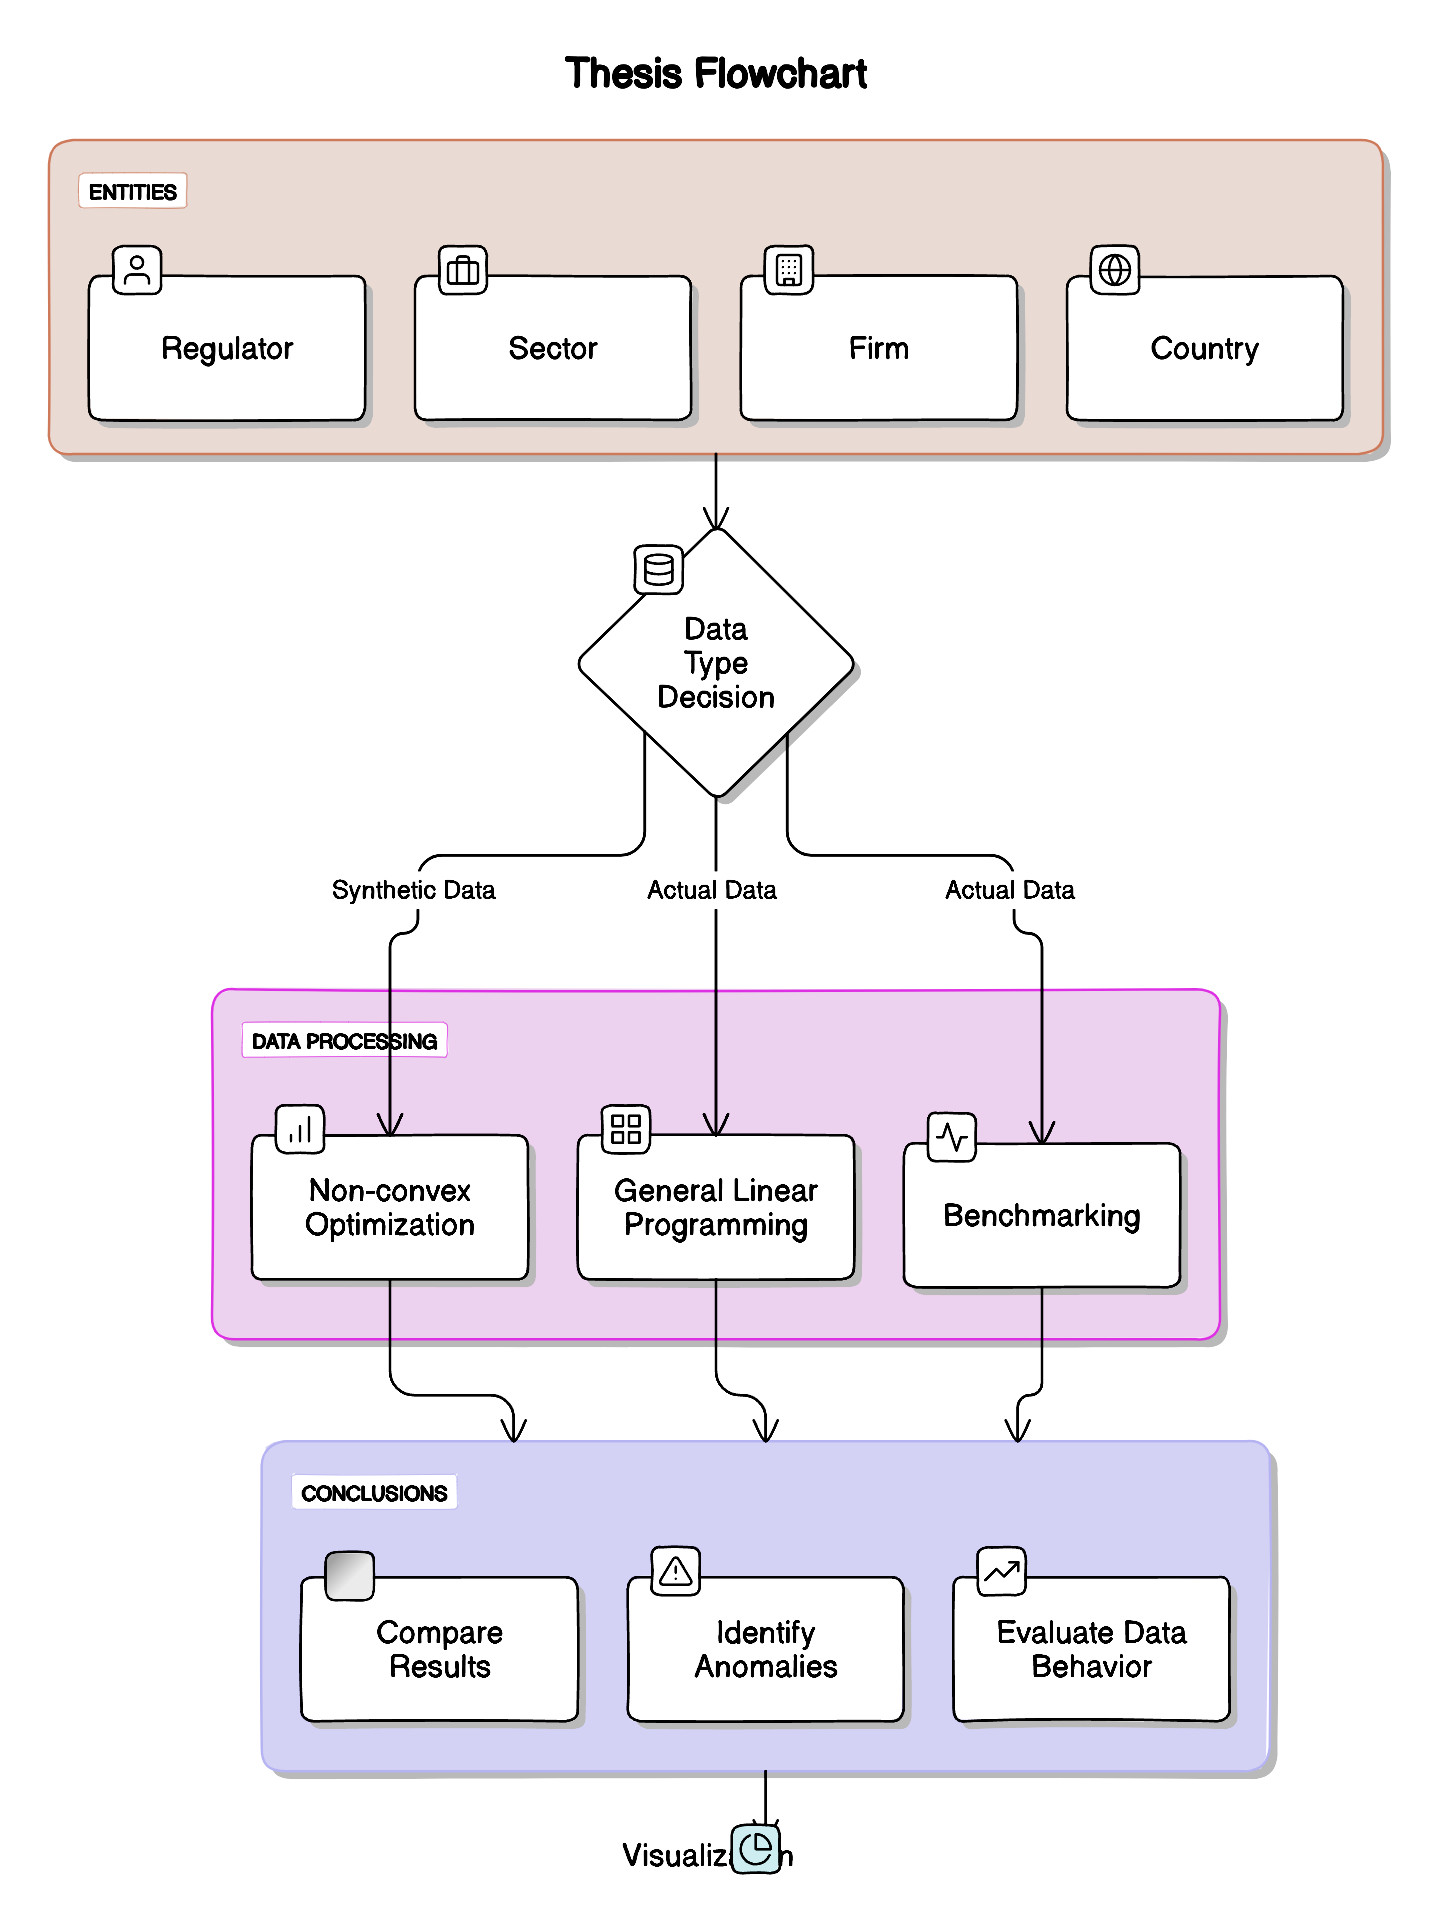
\includegraphics[width=0.7\linewidth]{images/diagram-export-8-28-2024-4_45_56-PM.jpg}
		\caption{}
		\label{fig:diagram-export-8-28-2024-44556-pm}
	\end{figure}
	\item \lbrack\_\rbrack 
	Προβλήματα και στόχοι για 29/8/24
	\begin{itemize}
		\item Βάζοντας κλάσεις και διαφορετικά sectors ξαφνικά δεν συγκλίνει το αποτέλεσμα αλλά μόλις φτάσει σχετικά κοντά αποτυγχάνει.
	\end{itemize}
	\begin{itemize}[label ={}]
	\item \lbrack \_ \rbrack Βάλε ακριβώς τις ίδιες συναρτήσεις με πριν και δες αν θα έχεις το ίδιο πρόβλημα.
	\item \lbrack \_ \rbrack Δοκίμασε αντί να λύνεις το πρόβλημα για κάθε εταιρεία ξεχωριστά να το λύνεις για όλες ταυτόχρονα με διαφορετικές μεταβλητές. 
	\item \lbrack \_ \rbrack Δοκίμασε να χωρίζεις την αντικειμενική συνάρτηση όπως κάνουν στο paper σε δύο βήματα που τα κάθε ένα μεγιστοποιεί κάτι άλλο. 
	\item \lbrack \_ \rbrack Παίξε με άλλες συναρτήσεις. Αύριο πρέπει να μπορείς να δείξεις κάτι που να λειτουργεί στην Τζέλα. 
	\item \lbrack \_ \rbrack Οπτικοποίησε τα δεδομένα. 
	
	\end{itemize}
	
	
	
	\end{itemize}












\section*{Πηγές, από 23/5/23}
\begin{thebibliography}{999}
	
	\bibitem{Guidance}
	Guidance on Interpretation of Annex I of the EU ETS Directive (excl. aviation activities),
	\url{https://www.mase.gov.it/sites/default/files/archivio/allegati/emission_trading/guidance_on_interpretation_annex_I_final.pdf}
	\bibitem{Nace1}
	NACE Codes: What Are They and Why Do They Always Matter?
	\url{https://connects.world/nace-codes/#What_are_NACE_codes_used_for}
	\bibitem{Allocating}
	Allocating Emission Permits Efficiently via Uniform Linear Mechanisms, \url{https://papers.ssrn.com/sol3/papers.cfm?abstract_id=4536951}
	\bibitem{First}
	DIMOS, S., FOTAKIS, D., MATHIOUDAKI, A., \& PAPADOPOULOS, K. Fair and Efficient Allocation of EU Emission Allowances. \url{https://cms.gnest.org/sites/default/files/Proceedings/cest2023_00077/cest2023_00077.pdf}
	\bibitem{Why}
	Why Nations Fail
	\url{https://edisciplinas.usp.br/pluginfile.php/3954893/mod_resource/content/0/Why-Nations-Fail-Daron-Acemoglu.pdf}
	\bibitem{'2269'}
	Ένα άρθρο που δεν έχει βγει ακόμα, αλλά ήρθε στον φωτάκη για review. Δεν το έχω διαθέσιμο, αλλά θα γίνει και ήταν πολύ καλό.
	

		
		
	
\end{thebibliography}

\section*{Παράρτημα Α'}\label{firstappendix}
Ας αρχίσω να έχω και τέτοια για να φαίνεται πιο μεγάλη αυτή η αναφορά.
Παραπομπή στον κώδικα της συνάρτησης sympy\_to\_gyrobi()
\begin{lstlisting}[language=Python, caption=Python example]
import sympy as sp
from gurobipy import Model, LinExpr, QuadExpr, GRB

# Define a function to convert SymPy expression to Gurobi expression
def sympy_to_gurobi(sympy_expr, symbol_map, model, aux_var_count=[0]):
	"""
	Recursively convert a SymPy expression to a Gurobi expression, 
	handling exponentials, powers, divisions, and other complex expressions with auxiliary variables and constraints.
	
	Parameters:
		sympy_expr (sp.Expr): SymPy expression to convert.
		symbol_map (dict): Mapping from SymPy symbols to Gurobi variables.
		model (gurobipy.Model): Gurobi model to add constraints for complex expressions.
		aux_var_count (list): A list to keep track of the auxiliary variable count.
		
	Returns:
		Gurobi expression (LinExpr, QuadExpr, or constant).
	"""
	if isinstance(sympy_expr, sp.Symbol):
		return symbol_map[sympy_expr]
	
	elif isinstance(sympy_expr, sp.Add):
		return sum(sympy_to_gurobi(arg, symbol_map, model, aux_var_count) for arg in sympy_expr.args)
	
	elif isinstance(sympy_expr, sp.Mul):
		result = 1
		for arg in sympy_expr.args:
			result *= sympy_to_gurobi(arg, symbol_map, model, aux_var_count)
		return result
	
	elif isinstance(sympy_expr, sp.Pow):
		base, exp = sympy_expr.args
		
		# Always create an auxiliary variable for the base
		base_expr = sympy_to_gurobi(base, symbol_map, model, aux_var_count)
		aux_var_name = f"pow_base_aux_{aux_var_count[0]}"
		aux_var_count[0] += 1
		base_aux_var = model.addVar(name=aux_var_name, vtype=GRB.CONTINUOUS)
		model.addConstr(base_aux_var == base_expr)
		
		if exp == 2:
			# Handle quadratic expression
			return QuadExpr(base_aux_var * base_aux_var)
		else:
			# Handle non-quadratic powers using general constraints
			exp_value = float(exp)
			aux_var_name = f"pow_aux_{aux_var_count[0]}"
			aux_var_count[0] += 1
			pow_aux_var = model.addVar(name=aux_var_name, vtype=GRB.CONTINUOUS)
			model.addGenConstrPow(base_aux_var, pow_aux_var, exp_value)
			return pow_aux_var
	
	elif isinstance(sympy_expr, sp.exp):
		arg_expr = sympy_to_gurobi(sympy_expr.args[0], symbol_map, model, aux_var_count)
		aux_var_name = f"exp_aux_{aux_var_count[0]}"
		aux_var_count[0] += 1
		arg_aux_var = model.addVar(name=f"aux_{aux_var_name}_arg", lb=0, vtype=GRB.CONTINUOUS)
		model.addConstr(arg_aux_var == arg_expr)
		exp_aux_var = model.addVar(name=aux_var_name, vtype=GRB.CONTINUOUS)
		model.addGenConstrExp(arg_aux_var, exp_aux_var)
		return exp_aux_var
	
	elif isinstance(sympy_expr, sp.log):
		arg_expr = sympy_to_gurobi(sympy_expr.args[0], symbol_map, model, aux_var_count)
		aux_var_name = f"log_aux_{aux_var_count[0]}"
		aux_var_count[0] += 1
		arg_aux_var = model.addVar(name=f"aux_{aux_var_name}_arg", vtype=GRB.CONTINUOUS)
		model.addConstr(arg_aux_var == arg_expr)
		log_aux_var = model.addVar(name=aux_var_name, vtype=GRB.CONTINUOUS)
		model.addGenConstrLog(arg_aux_var, log_aux_var)
		return log_aux_var

	elif isinstance(sympy_expr, sp.sin):
		arg_expr = sympy_to_gurobi(sympy_expr.args[0], symbol_map, model, aux_var_count)
		aux_var_name = f"sin_aux_{aux_var_count[0]}"
		aux_var_count[0] += 1
		arg_aux_var = model.addVar(name=f"aux_{aux_var_name}_arg", vtype=GRB.CONTINUOUS)
		model.addConstr(arg_aux_var == arg_expr)
		sin_aux_var = model.addVar(name=aux_var_name, vtype=GRB.CONTINUOUS)
		# Add piecewise constraints here for approximation
		return sin_aux_var

	elif isinstance(sympy_expr, sp.cos):
		arg_expr = sympy_to_gurobi(sympy_expr.args[0], symbol_map, model, aux_var_count)
		aux_var_name = f"cos_aux_{aux_var_count[0]}"
		aux_var_count[0] += 1
		arg_aux_var = model.addVar(name=f"aux_{aux_var_name}_arg", vtype=GRB.CONTINUOUS)
		model.addConstr(arg_aux_var == arg_expr)
		cos_aux_var = model.addVar(name=aux_var_name, vtype=GRB.CONTINUOUS)
		# Add piecewise constraints here for approximation
		return cos_aux_var

	elif isinstance(sympy_expr, sp.tan):
		arg_expr = sympy_to_gurobi(sympy_expr.args[0], symbol_map, model, aux_var_count)
		aux_var_name = f"tan_aux_{aux_var_count[0]}"
		aux_var_count[0] += 1
		arg_aux_var = model.addVar(name=f"aux_{aux_var_name}_arg", vtype=GRB.CONTINUOUS)
		model.addConstr(arg_aux_var == arg_expr)
		tan_aux_var = model.addVar(name=aux_var_name, vtype=GRB.CONTINUOUS)
		# Add piecewise constraints here for approximation
		return tan_aux_var

	elif isinstance(sympy_expr, sp.Mul) and any(isinstance(arg, sp.Pow) and arg.exp == -1 for arg in sympy_expr.args):
		# Handling division by separating numerator and denominator
		numerator = 1
		denominator = 1
		for arg in sympy_expr.args:
			if isinstance(arg, sp.Pow) and arg.exp == -1:
				denominator *= arg.base
			else:
				numerator *= arg
		
		# Handle numerator
		num_expr = sympy_to_gurobi(numerator, symbol_map, model, aux_var_count)
		num_aux_var_name = f"num_aux_{aux_var_count[0]}"
		aux_var_count[0] += 1
		num_aux_var = model.addVar(name=num_aux_var_name, vtype=GRB.CONTINUOUS)
		model.addConstr(num_aux_var == num_expr)
		
		# Handle denominator
		denom_expr = sympy_to_gurobi(denominator, symbol_map, model, aux_var_count)
		denom_aux_var_name = f"denom_aux_{aux_var_count[0]}"
		aux_var_count[0] += 1
		denom_aux_var = model.addVar(name=denom_aux_var_name, vtype=GRB.CONTINUOUS)
		model.addConstr(denom_aux_var == denom_expr)
		
		# Create the auxiliary variable for the inverse of the denominator
		inv_denom_aux_var_name = f"inv_denom_aux_{aux_var_count[0]}"
		aux_var_count[0] += 1
		inv_denom_aux_var = model.addVar(name=inv_denom_aux_var_name, vtype=GRB.CONTINUOUS)
		model.addConstr(inv_denom_aux_var * denom_aux_var == 1)
		
		# Final expression: numerator * (1/denominator)
		return num_aux_var * inv_denom_aux_var

	elif isinstance(sympy_expr, sp.Number):
		return float(sympy_expr)
	
	else:
		raise ValueError(f"Unsupported SymPy expression: {sympy_expr}")

\end{lstlisting}


\end{document}	